\chapter{Veto efficiency studies}\label{chap:VetoEfficiency}
A WIMP scatter is expected to only deposit a small amount of energy (few~keV) within the LXe volume of the experiment in a single scatter. Neutrons produced through radioactive decays within detector materials mimics a WIMP interaction when they scatter off Xe atoms. Veto detectors surrounding the central LXe volume also permits assessment of the local radioactivity environment, and thus to infer additional information on the backgrounds in the WIMP search region. A WIMP discovery will require excellent understanding of all background sources, which is best done through the characterization of those backgrounds in situ. Efficiency of the veto systems in the detection of the radiation produced by the backgrounds should be maximised whilst minimizing the impact of the veto selection on detector livetime in turn maximising the detector livetime available for the detection of WIMPs. \autoref{sec:VetoEff/simulation_improvements} describes the series of improvements to the detector simulation which were made prior to the WS2024 science run which aided the understanding of the response from the veto detector systems. The refinement of the veto selection algorithm is discussed alongside the impact that the veto selection had on the WS2024 result from \autoref{sec:VetoEff/VetoSelectionOptimisation} onwards.

\section{Simulation matching}\label{sec:VetoEff/simulation_improvements}
\subsection{Tuning the OD simulations}
\subsubsection{Geometry edits}\label{sec:VetoEff/GeometryEdits}
Prior to WS2024 result, there were a number of major differences between simulations and data in the Outer Detector (OD).
There was a distinct discrepancy in neutron capture timing following single scatters within the TPC, this was one of the metrics which was investigated to quantify difference between data and simulation.
The simulation was improved through the following changes:
\begin{enumerate}
	%\item Spacing was added between the acrylic tanks to account for the gaps between the tanks which were present due to minor geometric differences produces in the moulding of the vessels during manufacturing process.
	\item Water was added to the foam volume which is between the OCV and acrylic tanks. The foam was intended to displace water to reduce neutron capture time however the foam became saturated with water \footnote{Later long-term bench top studies found that samples of foam became saturated with water.}.
	\item The acrylic tanks were moved further away from the OCV to replicate the actual position of the tanks in the Outer Detector.
\end{enumerate}
A series of simulations were produced varying both the amount of water saturation of foam displacer in 1\% steps and the position of the acrylic tanks from the OCV in 10~mm steps. The \textit{best} configuration of the simulation geometry changes was found to be 30~mm and 6\% through matching the capture time of neutrons following single scatters in the active LXe volume. Additional details on the discrepancies between simulations and data with respect to neutron capture timing is given in the subsequent subsection.
\begin{figure}[ht!]
	\centering
	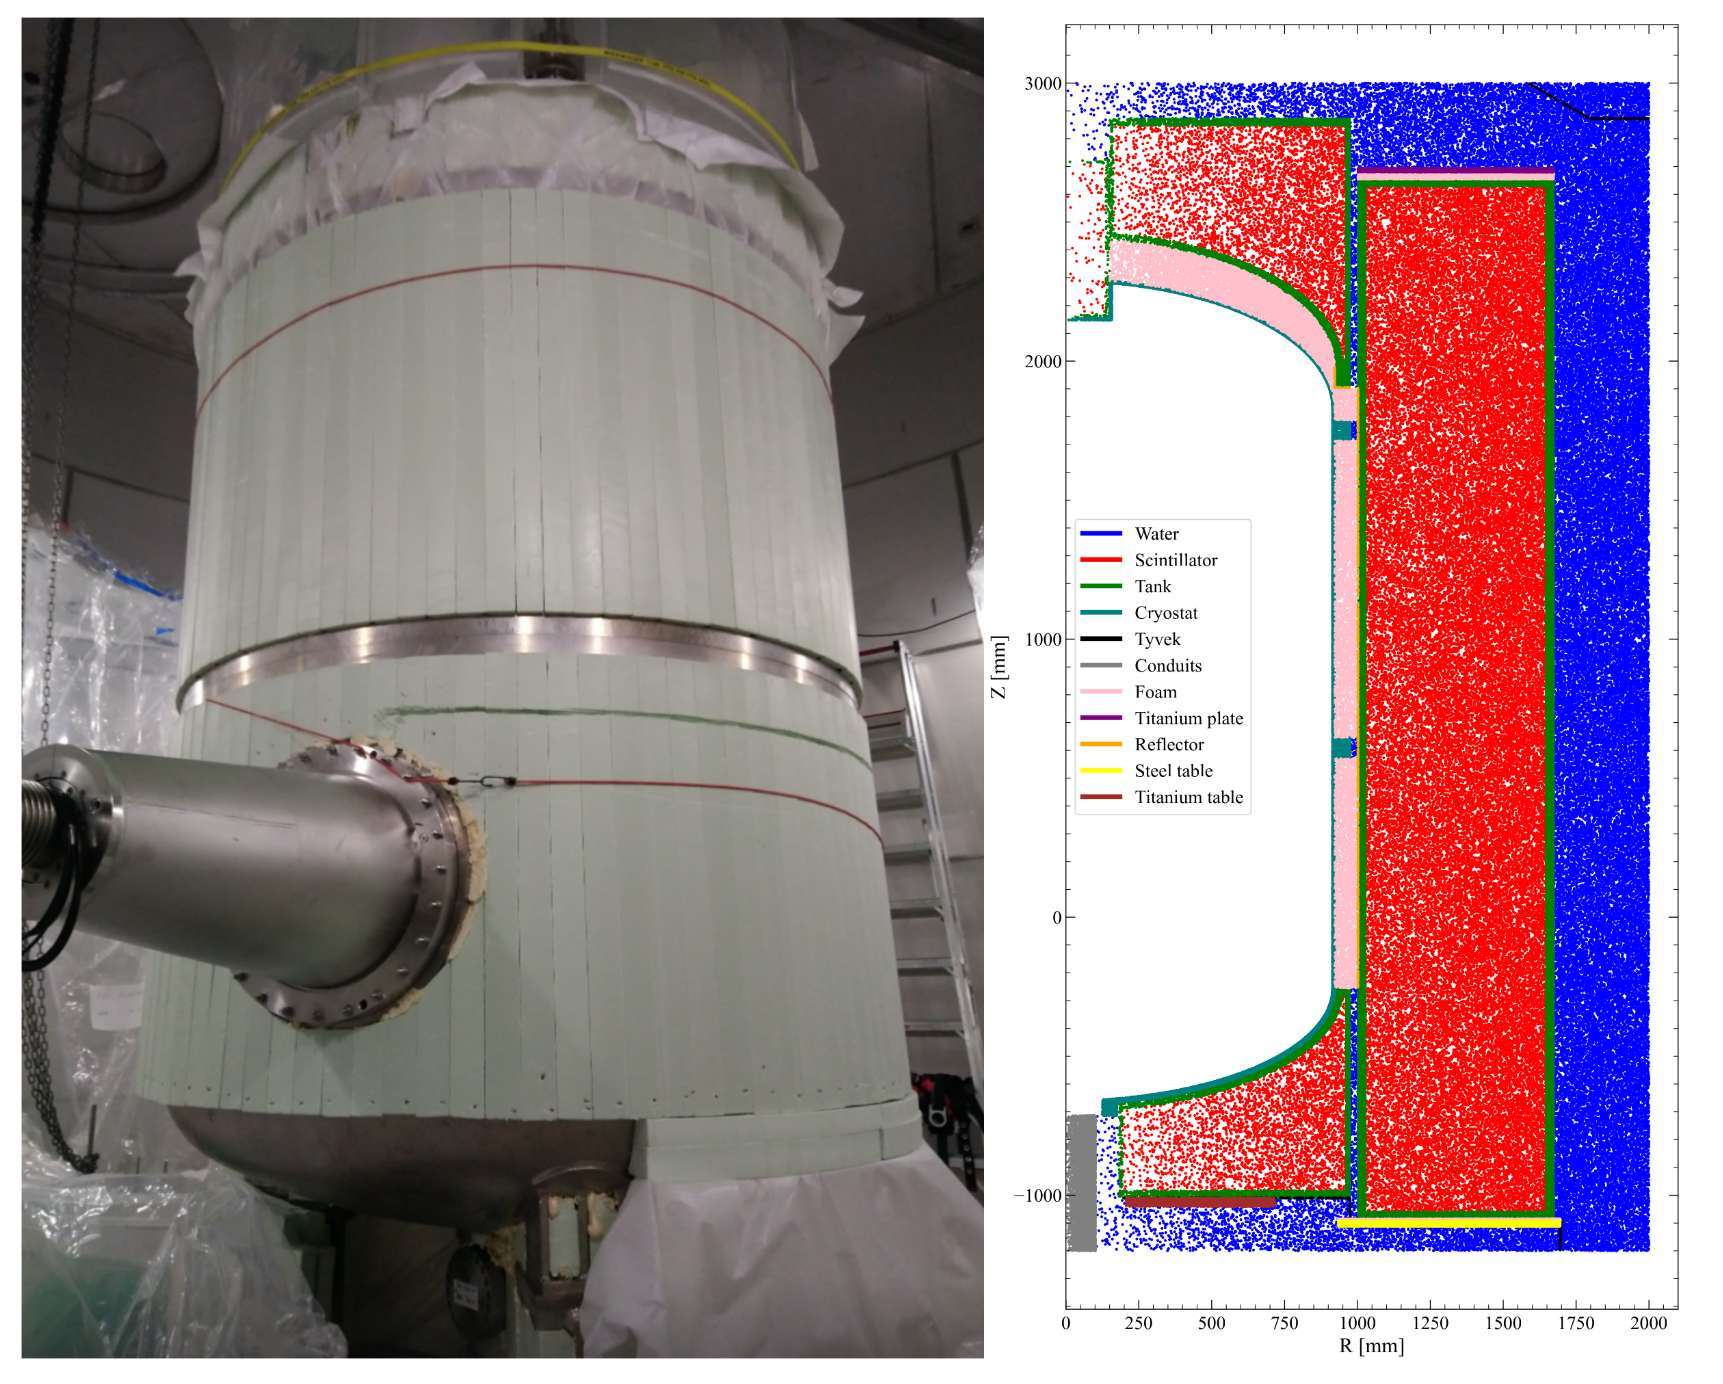
\includegraphics[width=0.9\textwidth]{figures/VetoEfficiency/FoamImgAndSimGeoTogether.png}
	\caption[An image of the foam displacer surrounding the OCS and final geometry in the simulation used for the WS2024 science run.]{Geometry in the simulation used for the WS2024 science run. \textbf{Left:} A photograph of the light green foam water displacer which resides between the acrylic tanks and the OCV. The water displacer was wrapped in a light reflector made from Tyvek. \textbf{Right:} A cross-section of the BACCARAT output. Geantinos were been passed through the simulation geometry, the $xyz$ position information and GEANT4 volumes were recorded to show the various volumes in the simulation.}
	\label{fig:VetoEff/od_geometry_for_sr3}
\end{figure}

\subsubsection{Neutron capture time}\label{sec:VetoEff/NCT}
Following the geometry changes discussed above, the neutron capture timing using AmLi was studied. Events which were classified as single scatters by LZap and passed the selection outlined in \autoref{tab:CoreCuts} in \autoref{app:CoreCutsTable} were used for the study. OD pulses which exceeded a 200~keV (49~phd) threshold were used to optimise the geometry as this threshold is associated with proton recoil of neutrons of hydrogen in the OD medium.
All possible configurations of the geometry modifications were visually examined to determine which variation of simulation matched the data. An example of the comparison plot can be seen in \autoref{fig:VetoEff/NC_AmLi_50mm7}, the "baseline simulation" was the initially configuration of the geometry prior to this study. All plots were examined side by side in a large scale canvas configuration seen in Fig.\ref{fig:VetoEff/NC_Canvas0}, \ref{fig:VetoEff/NC_Canvas1}, \ref{fig:VetoEff/NC_Canvas2}, and \ref{fig:VetoEff/NC_Canvas3} in \autoref{app:NC_Canvases}. It was found that from this study that 30~mm~to~50~mm movement of the SATs alongside 5\%~to~7\% increase in the percentage of water in the foam provides the best agreement between data and simulation at a 200~keV threshold.
\begin{figure}[!ht]
	\centering
	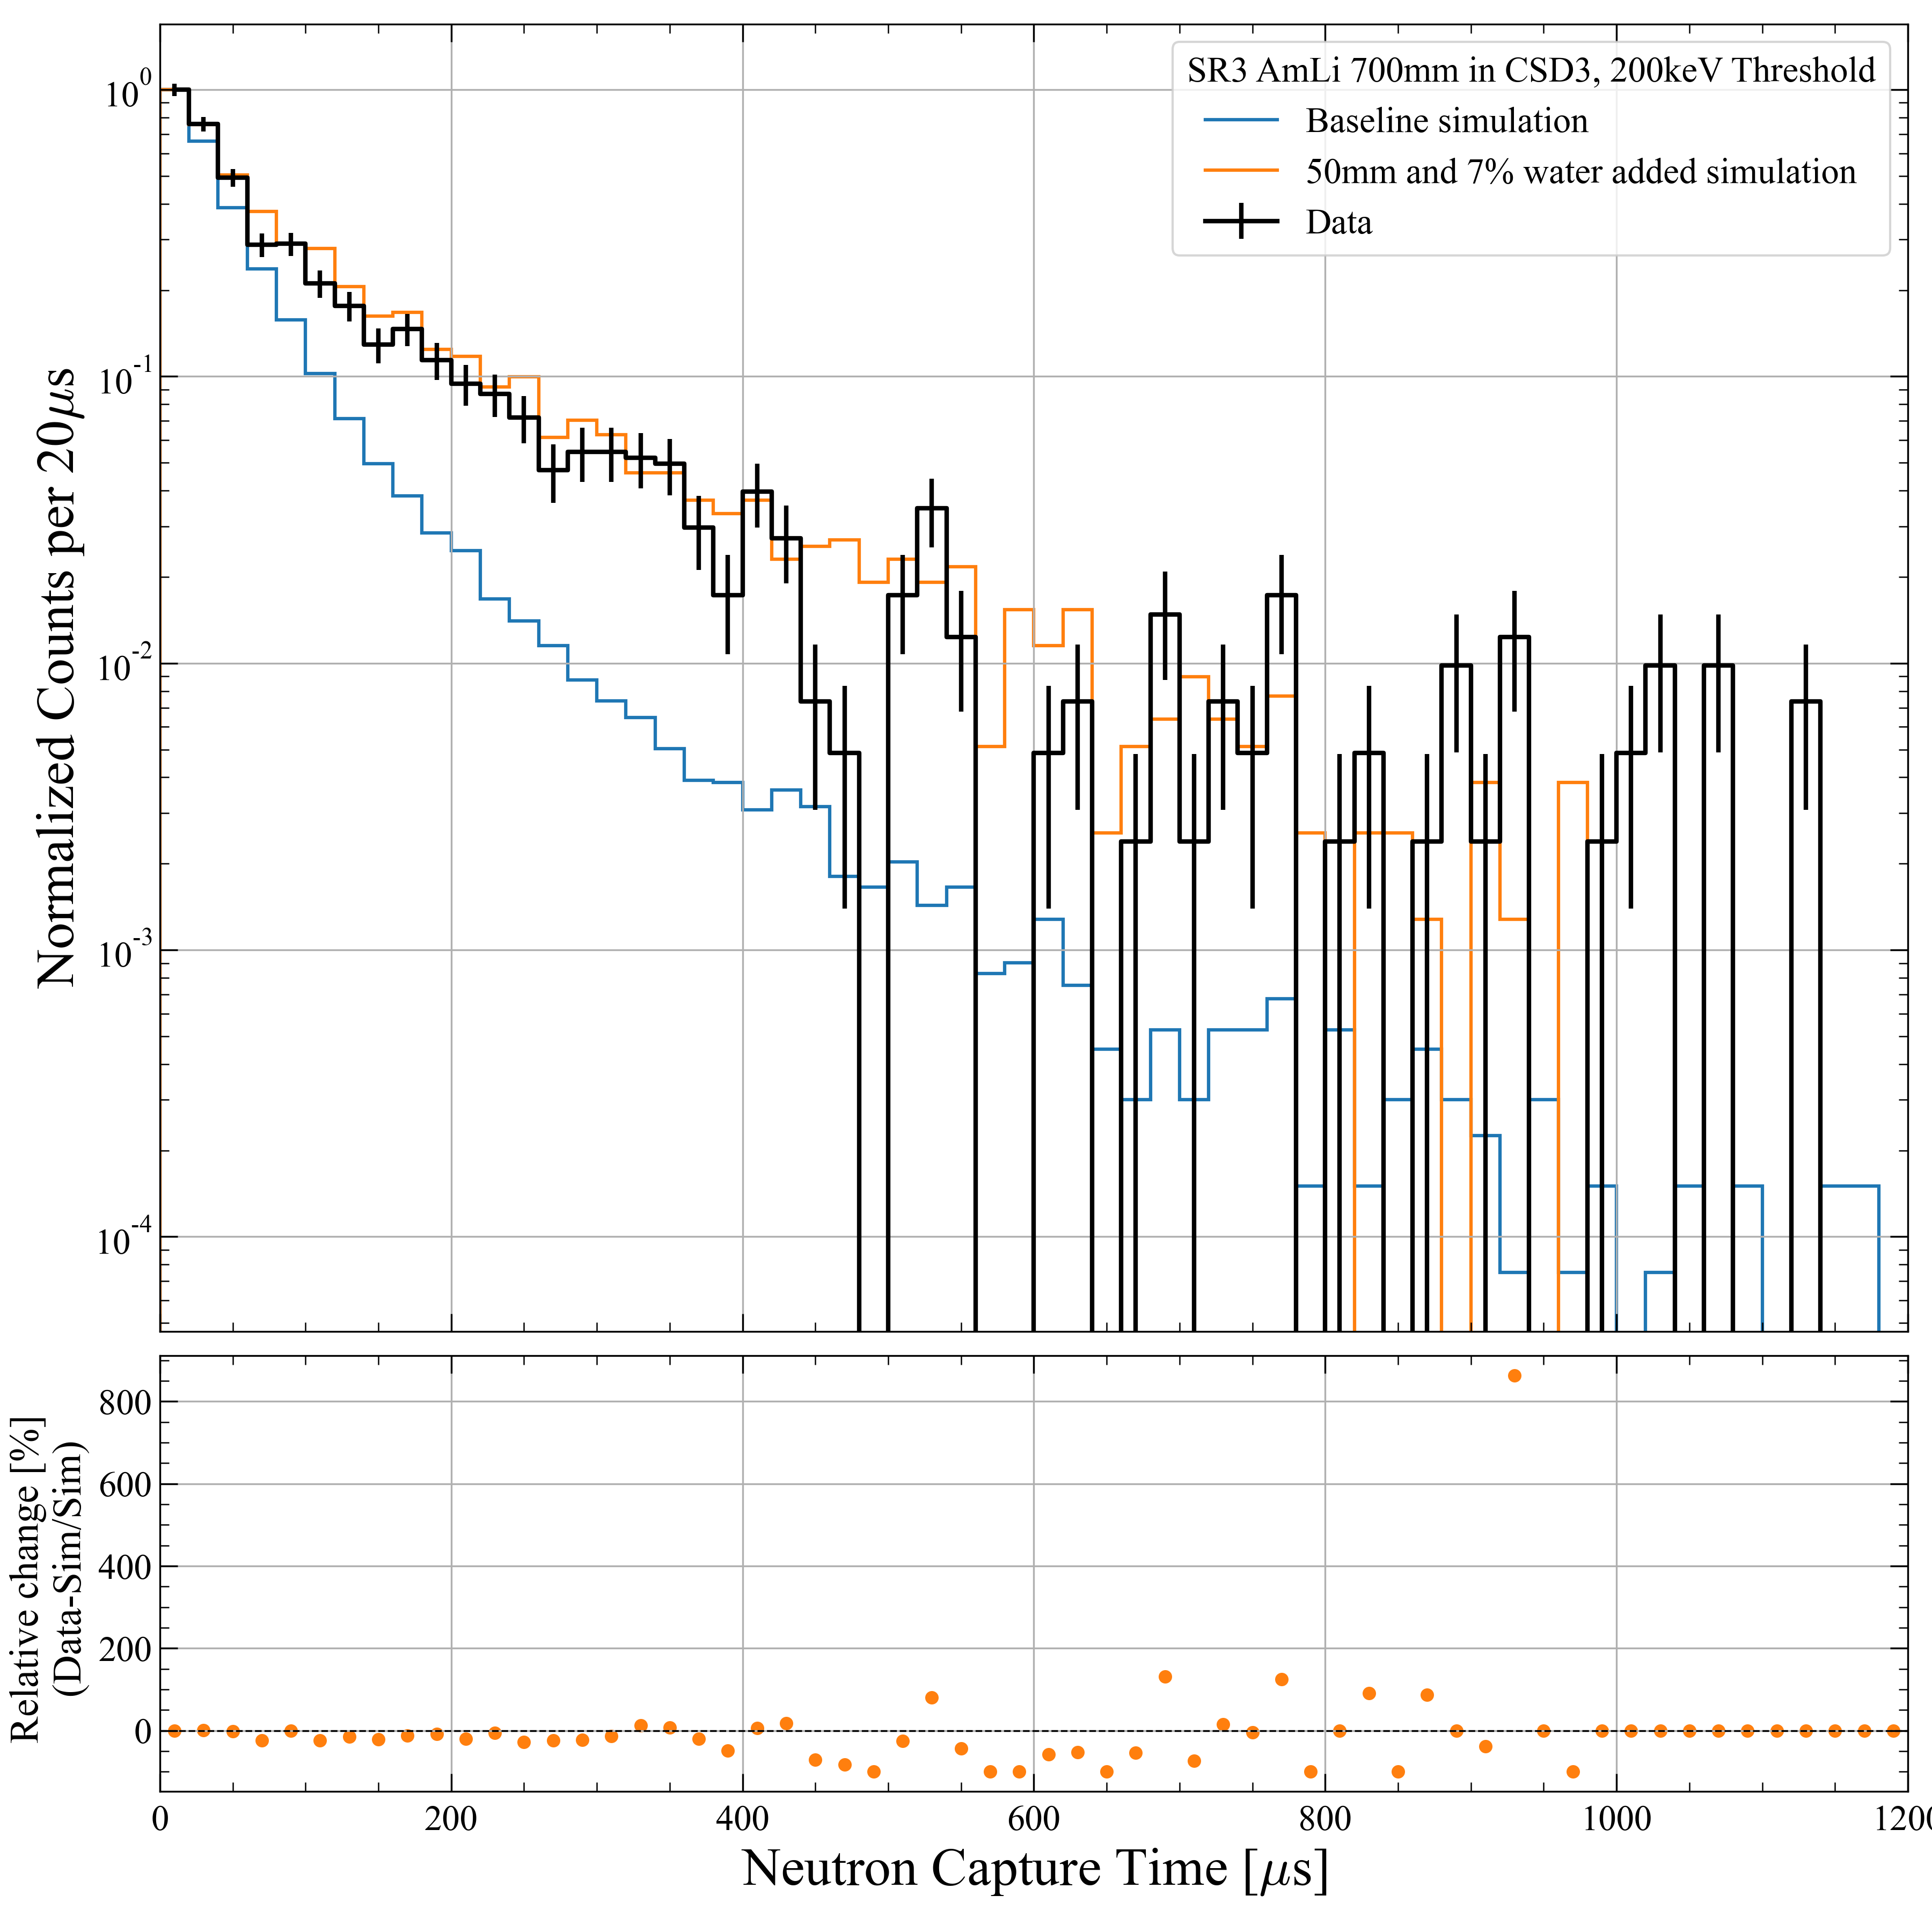
\includegraphics[width=0.7\linewidth]{figures/VetoEfficiency/movedSAT50mm_7percentWater_AmLi_CSD3_Z700mm_200keV_Ratio.png}
	\caption{An example of the plot used to compare neutron capture timing in data with the baseline simulation and the modified simulation. The relative change between data and simulation in each $20~\mu s$ bin was used to aid the visually examination across the $1200~\mu s$ window.}
	\label{fig:VetoEff/NC_AmLi_50mm7}
\end{figure}

\iffalse
\begin{sidewaysfigure}[ht!]
	\centering
	\includegraphics[width=\linewidth]{figures/VetoEfficiency/NCTiming_Canvas_700mm_AmLi.pdf}
	\caption{Large scale canvas of all possible simulation configurations. Each plot is similar in style to \autoref{fig:VetoEff/NC_AmLi_50mm7}. Here AmLi at 700mm above the cathode in CSD3 has been shown as an example.}
	\label{fig:VetoEff/NC_Canvas}
\end{sidewaysfigure}
\fi

\section{Veto selection optimisation}\label{sec:VetoEff/VetoSelectionOptimisation}
A description of how the veto selection for the WS2024 was optimised is presented in this section. The Skin and OD veto cuts used in the WS2024 science run were based on those developed for the WS2022 science run, described in \cite{LZCollaboration:2024lux} and are presented in \autoref{tab:VetoEff/sr3_veto_cuts}.
The veto selection relies on four separate selection criteria which each have their own intended purposes:
\begin{itemize}
	\item \textit{Skin-prompt} used for tagging $\gamma$-rays in the Skin detector
	\item \textit{OD-prompt} used for tagging $\gamma$-rays and neutron proton recoils in the OD
	\item \textit{Skin-delayed} used for tagging $\gamma$-rays from post-neutron capture de-excitation
	\item \textit{OD-delayed} used For tagging $\gamma$-rays from post-neutron capture de-excitation
\end{itemize}
The cuts used for the different veto criteria were selected at the same time as AmLi neutron tagging efficiency calculation, and were optimised to maximise the tagging efficiency whilst reducing deadtime. \textit{Pulse area} threshold, \textit{PMT coincidence} threshold and \textit{veto window length} are the three different variables which can be tuned for this optimisation. Events which were classified as single scatters by LZap and passed the selection outlined in \autoref{tab:CoreCuts} in \autoref{app:CoreCutsTable} were used for the study. The following subsections describe how each of the veto selection variables were tuned.

\begin{table}[!ht]
	\centering
	\caption{Outline of cuts applied to AmLi calibration data for determining the veto efficiency. All cuts are defined in \autoref{tab:CoreCuts} in \autoref{app:CoreCutsTable}.}
	\label{tab:VetoEff/amli_efficiency_cuts}
    \scalebox{0.9}{
	\begin{tabular}{llll}
    \hline\hline
    \textbf{Livetime cuts}&\textbf{ Physics cuts}& \textbf{S1 cuts}& \textbf{S2 cuts}\\
    \hline
    Burst noise cut& Single scatter& S2 width vs drift time& S1 prominence cut\\
    Muon holdoff& S1 and S2 threshold & Narrow S2& Stinger event cut\\
    Sustained rate cut& Fiducial Volume& S2 rise time& S1 TBA vs drift time \\
    High S1 rate exclusion & & S2 early peak& S1 HSC cut\\
    Bad buffer cuts& & S2 XY quality& S1 shape\\
    Excess Area cut& & S2 TBA & S1 photon timing\\
    \hline\hline
	\end{tabular}}
\end{table}

\subsection{Veto window length}
The veto window length for the prompt windows were determined using AmLi and DD calibration data by measuring the time difference between the TPC single-scatter and OD and Skin pulses. The length of the prompt window is determined by width of the peak observed in the pulse timing distributions shown in both figures in \autoref{fig:VetoEff/veto_prompt_windows}. For the WS2024 selection, no change was made to the OD prompt veto window size, however the Skin prompt veto window was reduced by 500~ns as the number of the pulses observed outside of window $\pm250$~ns was considered negligible.
\begin{figure}[!ht]
	\centering
	\begin{subfigure}[b]{0.48\textwidth}
		\centering
		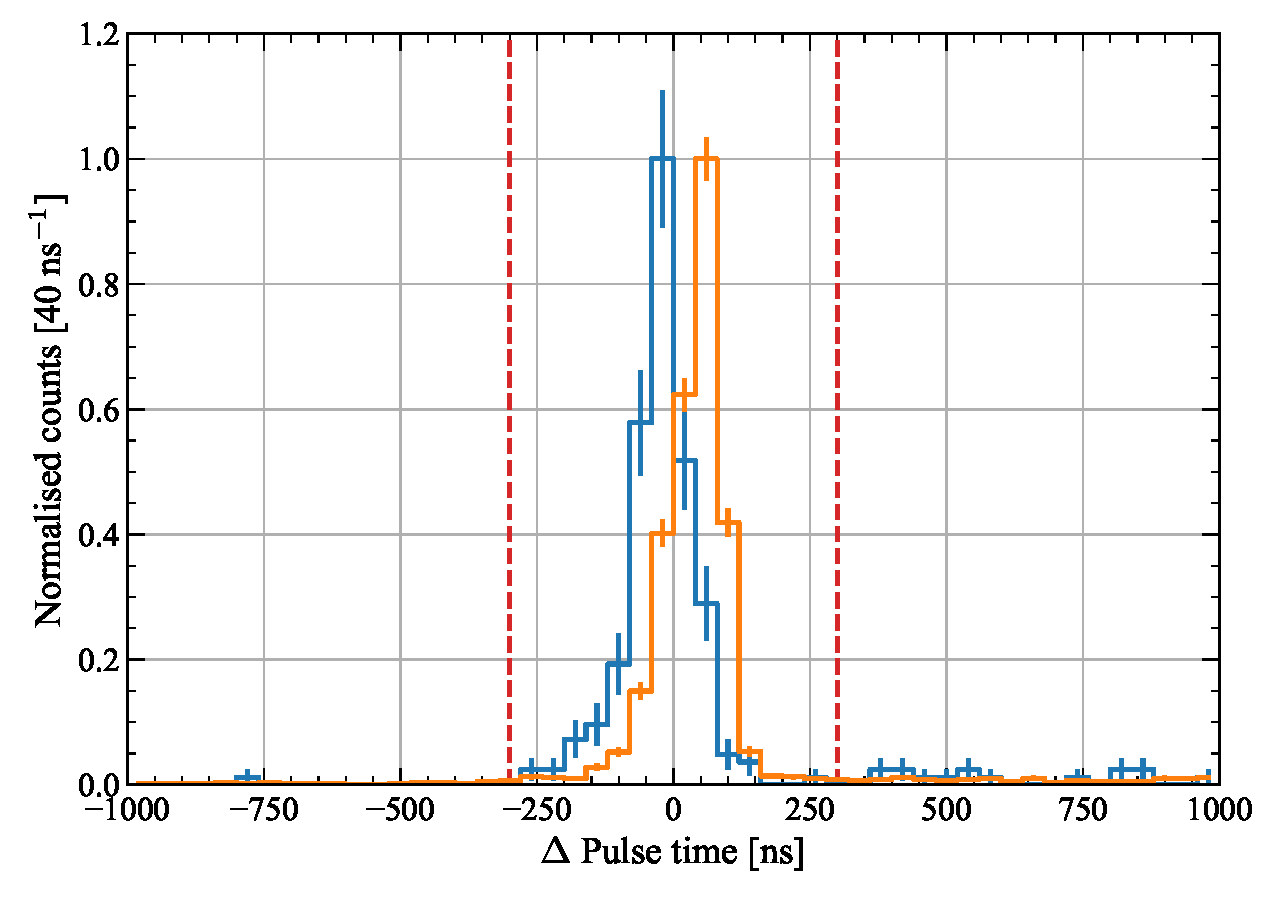
\includegraphics[width=\textwidth]{figures/VetoEfficiency/ODpromptWindowTiming.pdf}
		%\caption{Time difference (in ns) between TPC single-scatter and OD pulses using AmLi data.}
        \caption{}
		\label{fig:VetoEff/od_prompt_window}
	\end{subfigure}
	\hfill
	\begin{subfigure}[b]{0.48\textwidth}
		\centering
		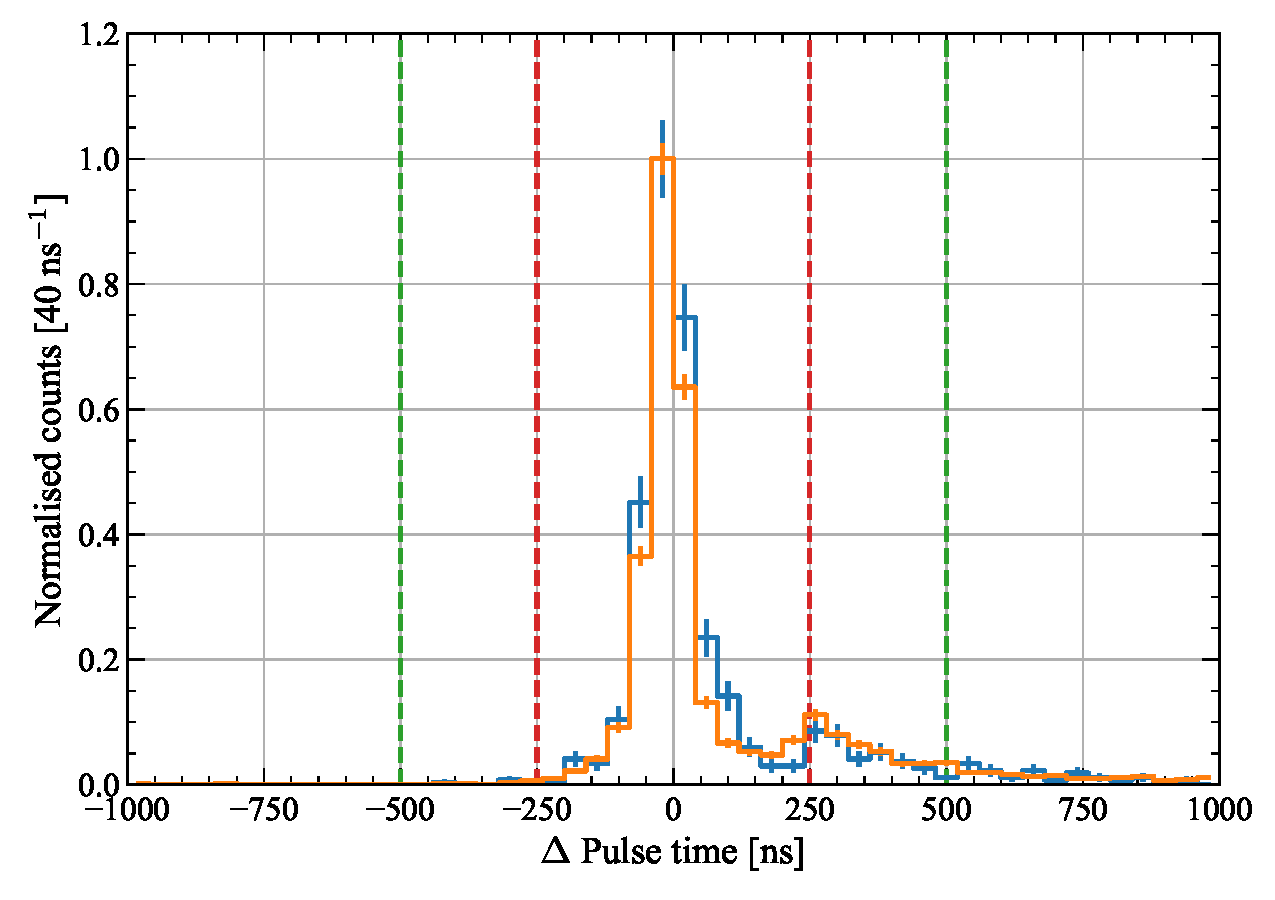
\includegraphics[width=\textwidth]{figures/VetoEfficiency/SkinpromptWindowTiming.pdf}
		%\caption{Time difference (in ns) between TPC single-scatter and OD pulses using DD data.}
		\caption{}
        \label{fig:VetoEff/skin_prompt_window}
	\end{subfigure}
	\caption{Prompt timing window for the OD (left) and Skin (right). %The time difference between TPC single scatter pulse and veto pulse was used to determine the optimal veto window size. 
    AmLi (blue) and DD (orange) calibration data was used to measure the time difference between the TPC single scatter pulse and veto pulse. 
    The vertical red lines indicate the boundary of the timing selection used for WS2024. There was no change in the size of the OD prompt veto window whereas the Skin prompt veto window was reduce by a total of 500~ns. The WS2022 veto window limits are shown in green.}
	\label{fig:VetoEff/veto_prompt_windows}
\end{figure}

The veto efficiency (defined in \ref{eqn:VetoEff/:neutron_tagging_efficiency}) calculated using AmLi calibration data was used to determine the size of the delayed veto window for both the Skin and OD. The veto window length was reduced by a factor of two for both Skin and OD delayed windows as the slope of the efficiency curve began to plateau above 600~$\mu s$. An example of the veto efficiency plot used is shown in \autoref{fig:VetoEff/DelayedVetoWindow}.
\begin{figure}[!ht]
    \centering
    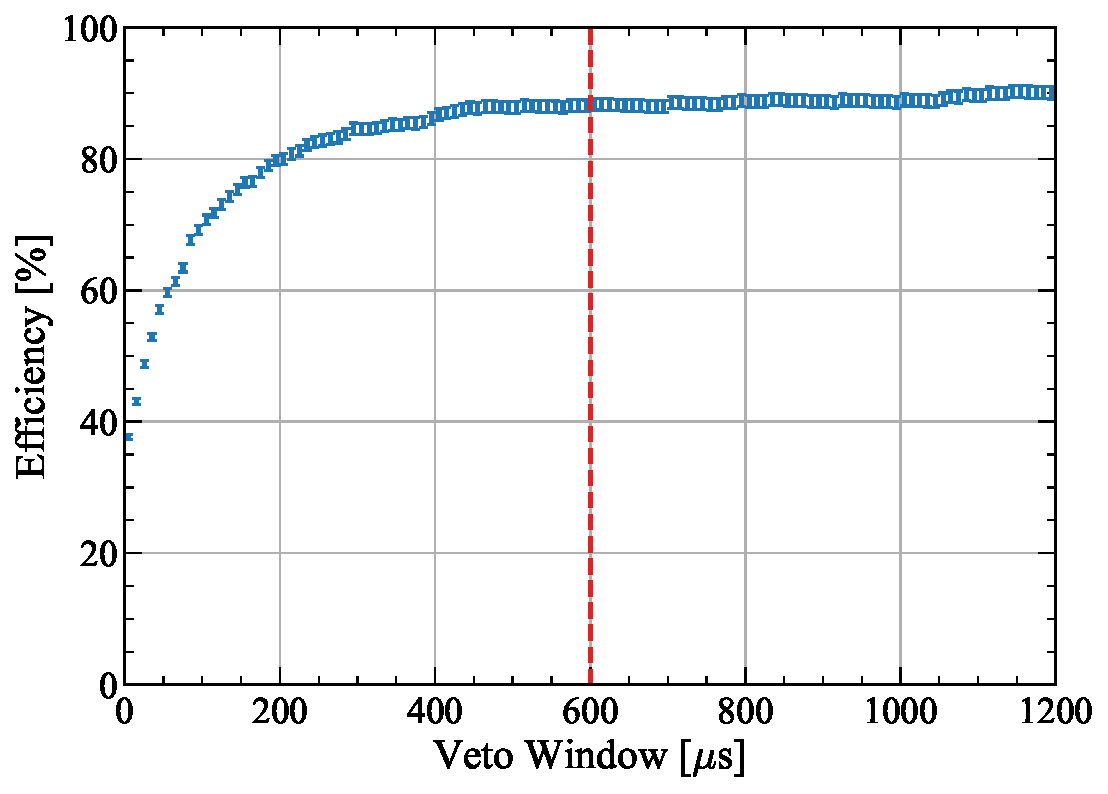
\includegraphics[width=0.5\linewidth]{figures/VetoEfficiency/DelayedVetoWindow.pdf}
    \caption{An example of a veto efficiency curve measured using AmLi calibration data. The vertical red line indicates the WS2024 upper bound of the delayed veto windows used for both the Skin and OD.}
    \label{fig:VetoEff/DelayedVetoWindow}
\end{figure}

The reduction in the veto window lengths has a positive impact on the dead time induced by the veto selection. Veto dead time is discussed in greater detail \autoref{sec:VetoEff/DeadtimeStability}.

\subsection{PMT Coincidence and pulse area threshold}
To optimize the pulse area and PMT coincidence thresholds the veto efficiency and deadtime was calculated for different integer step changes of both the pulse area and PMT coincidence for the respective veto windows. Heatmaps of efficiency and deadtime based on PMT coincidence and pulse area threshold were produced, an example of a heatmap is shown in \autoref{fig:VetoEff/od_prompt_veto_heatmap}. All heatmaps produced for the optimization study are shown in \autoref{app:VetoHeatMaps}.

\begin{sidewaysfigure}
	\centering
	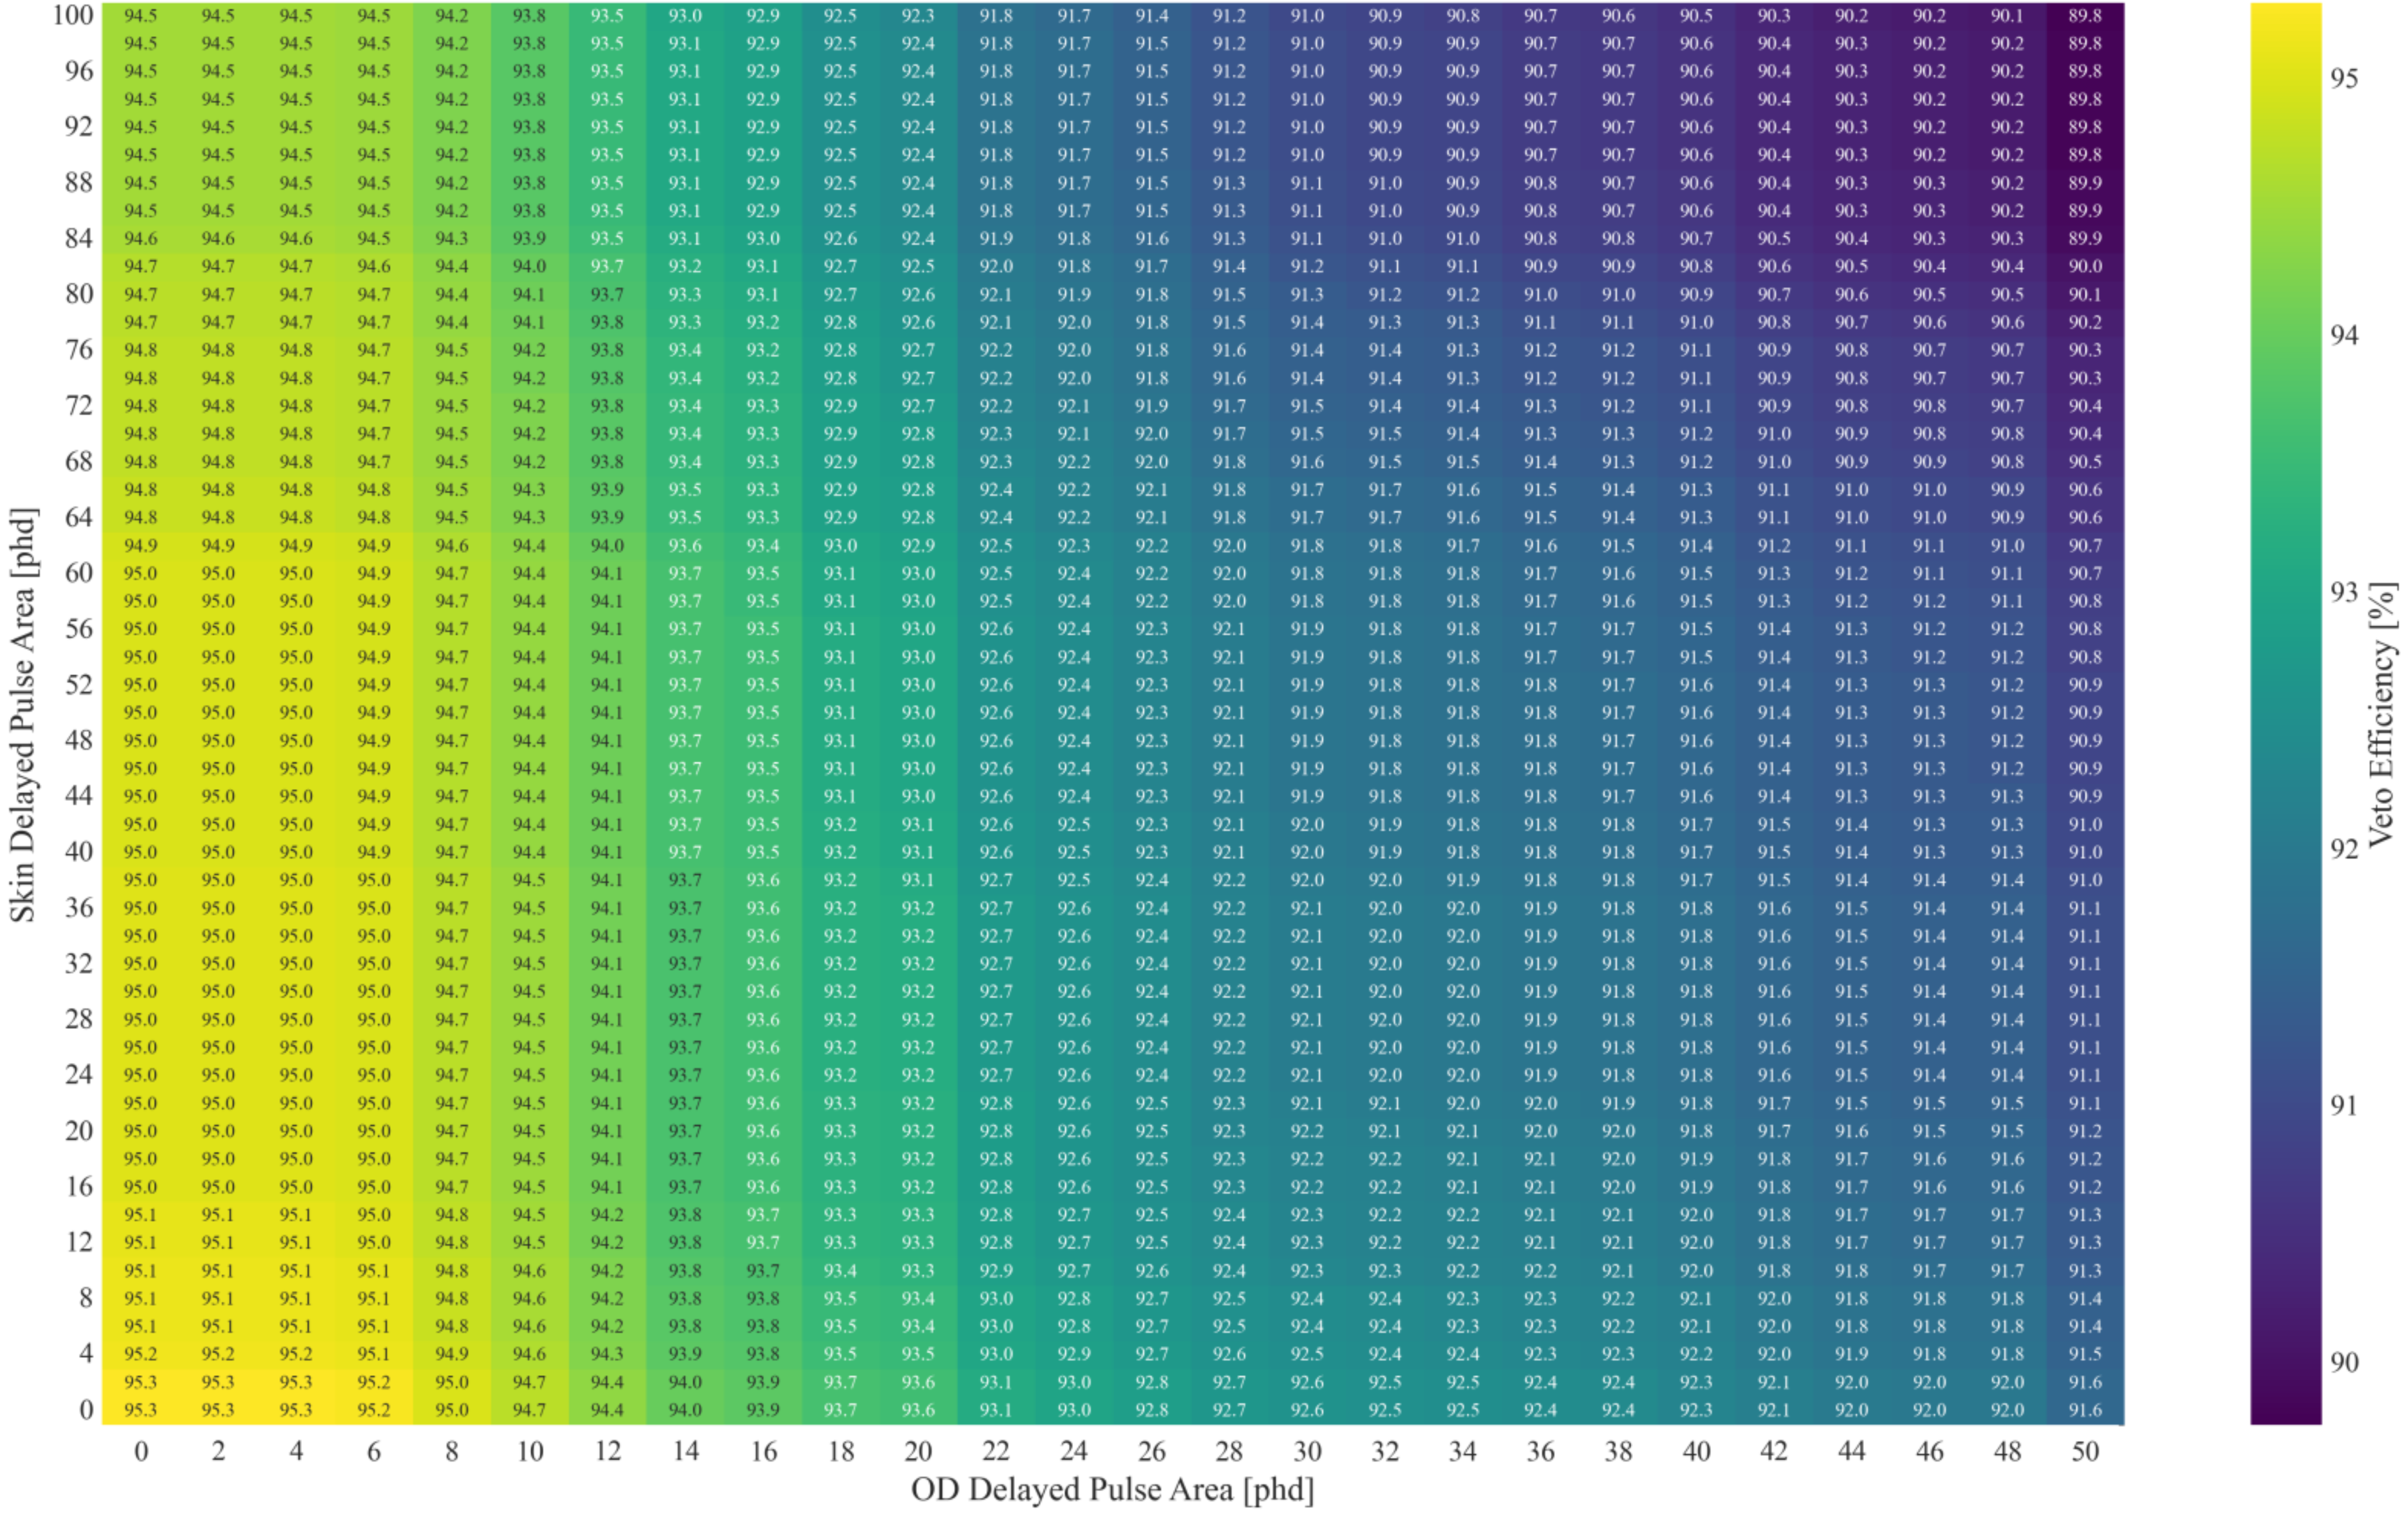
\includegraphics[width=\textwidth]{figures/VetoEfficiency/Heatmap600us_ODDelayedSkinDelayedThresholds.png}
	\caption{Heatmap used to determine optimal OD and Skin Delayed thresholds based on efficiency.
		The z-axis shows the efficiency associated with a given pulse area requirement for the delayed veto windows defined in \autoref{tab:VetoEff/sr3_veto_cuts}.
	}
	\label{fig:VetoEff/od_prompt_veto_heatmap}
\end{sidewaysfigure}

Compiling the heatmaps of efficiency and deadtime for established veto windows of the different criteria, thresholds were chosen to maximise efficiency whilst minimising dead time. An example plot used to determine this is shown in \autoref{fig:VetoEff/veto_cut_optimisation}.
For the WS2024 science run, the approach of trying to maintain the efficiency of WS2022 veto of $\sim$~89\%, whilst reducing the livetime impact was taken. It was determined that the efficiency could be matched to the veto efficiency achieved in the WS2022 science run whilst achieving a factor of two reduction in deadtime.

\noindent
The final cuts for the WS2024 science run are shown in \autoref{tab:VetoEff/sr3_veto_cuts}, with the WS2022 selection included for comparison.

\iffalse
\begin{sidewaysfigure}
	\centering
	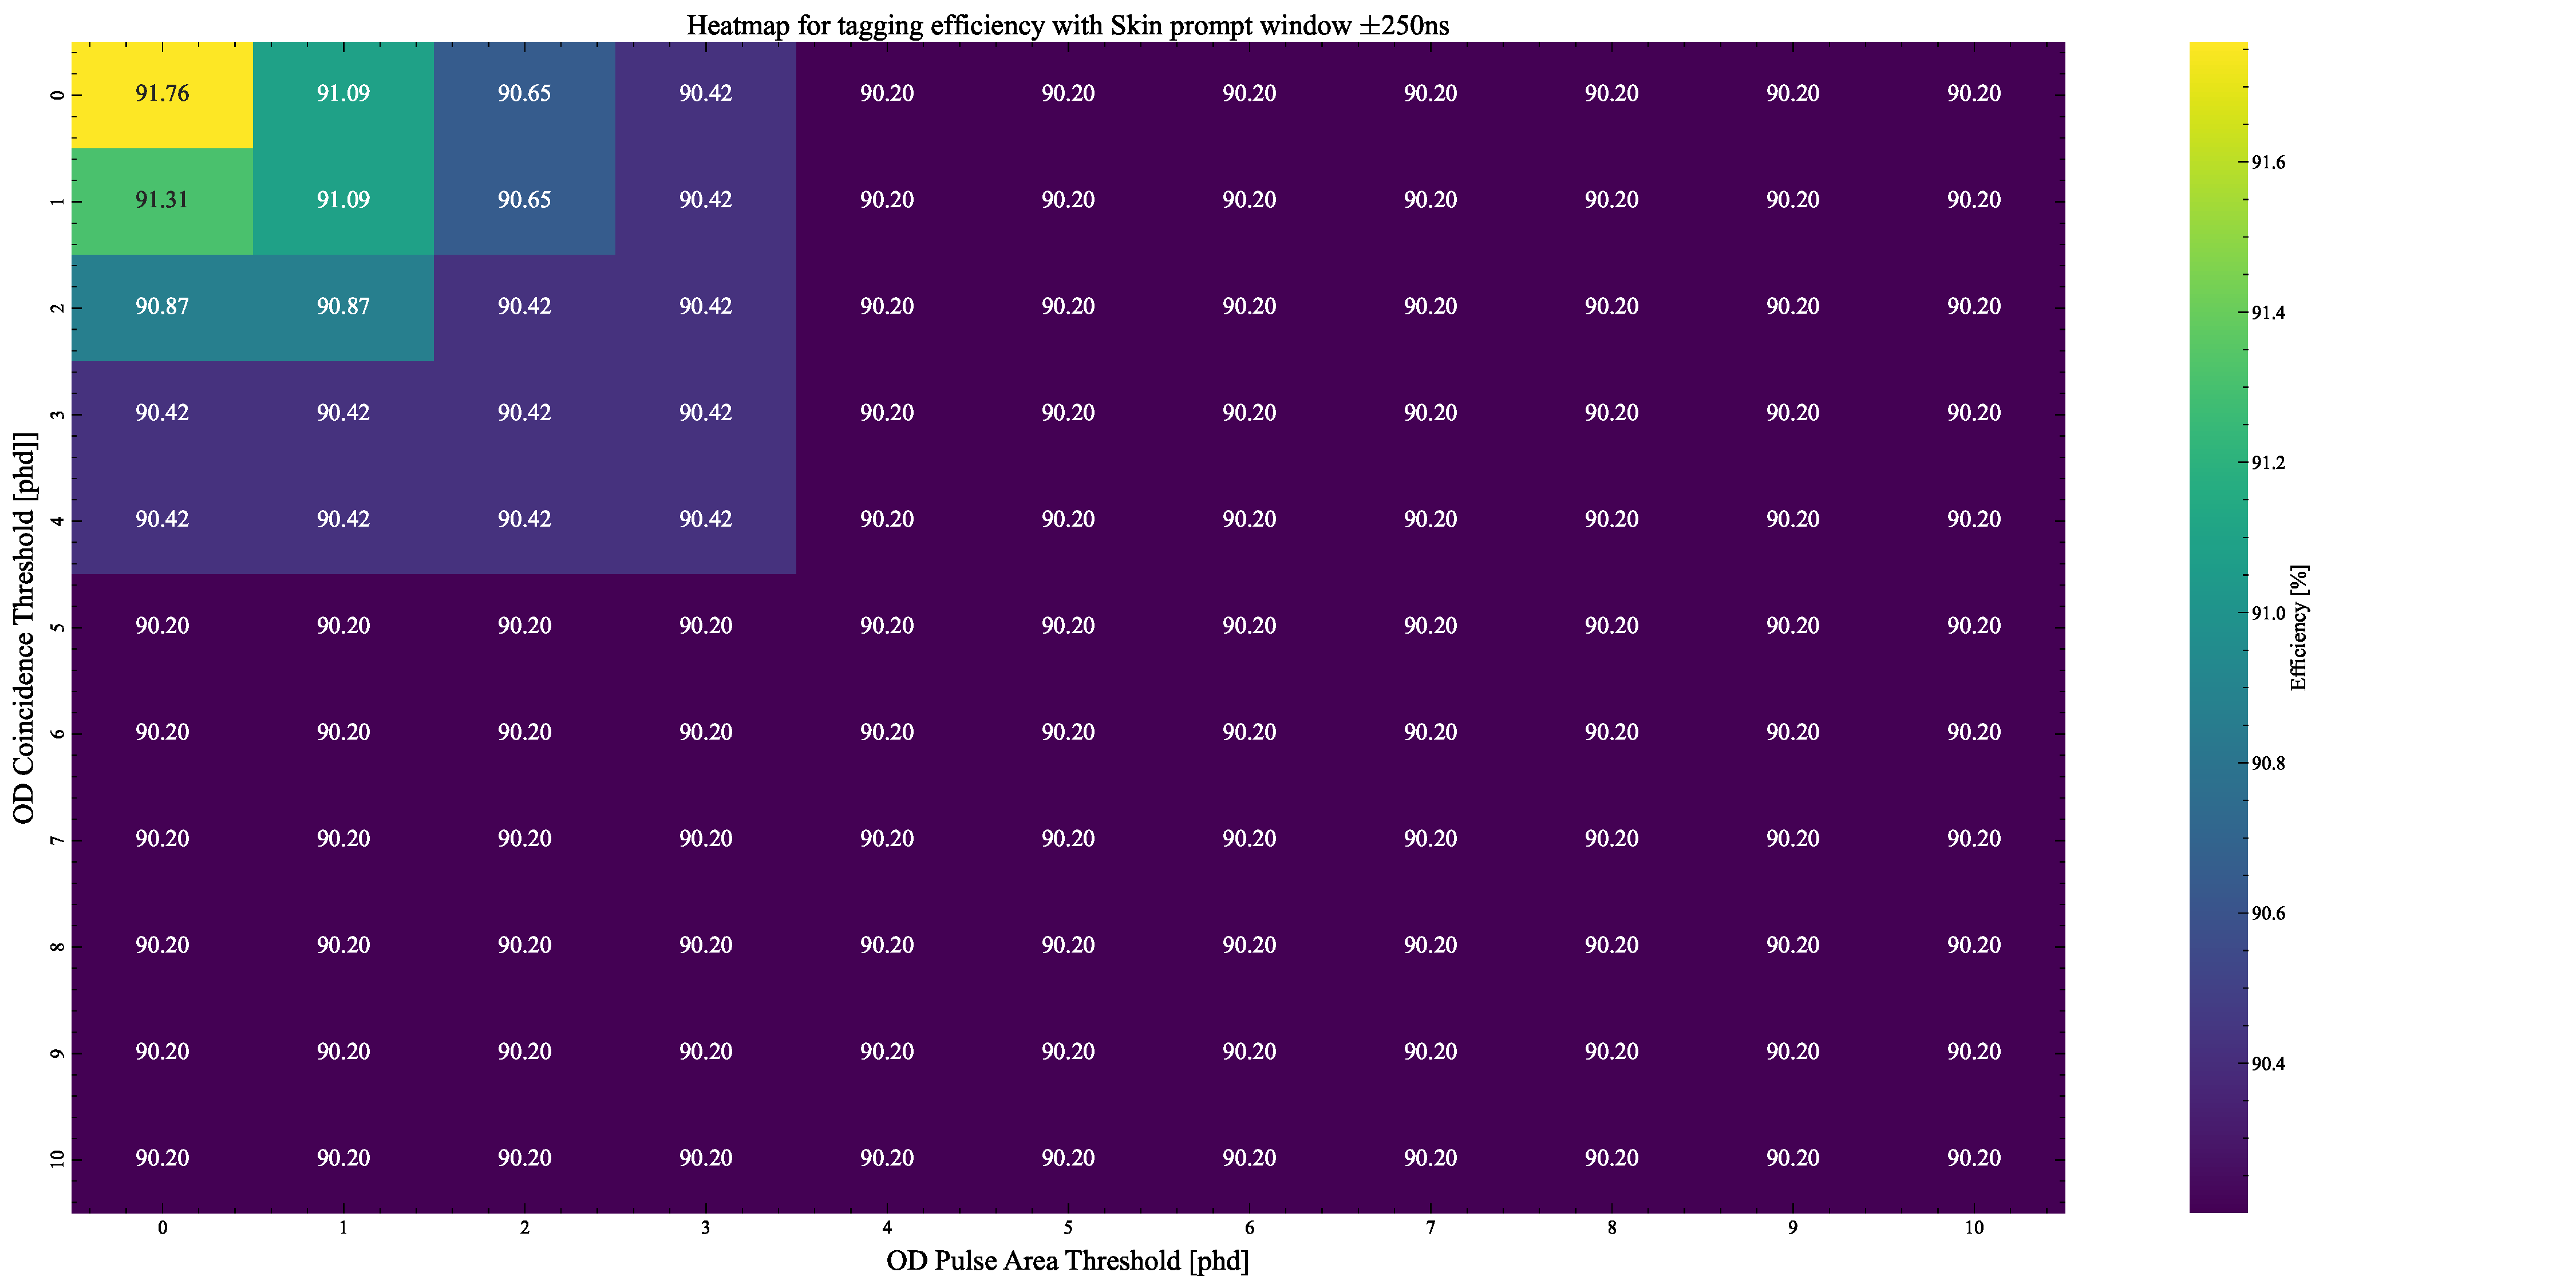
\includegraphics[width=\textwidth]{figures/VetoEfficiency/HeatmapSkinPACoinScanWindow500.pdf}
	\caption{Skin Prompt heatmap.
		In each bin, either the pulse coincidence or the pulse threshold has been varied.
		The z-axis shows the efficiency associated with a given pulse requirement.
		The veto time window considered is [-250, 250]ns.}
	\label{fig:VetoEff/skin_prompt_veto_heatmap}
\end{sidewaysfigure}
\begin{sidewaysfigure}
	\centering
	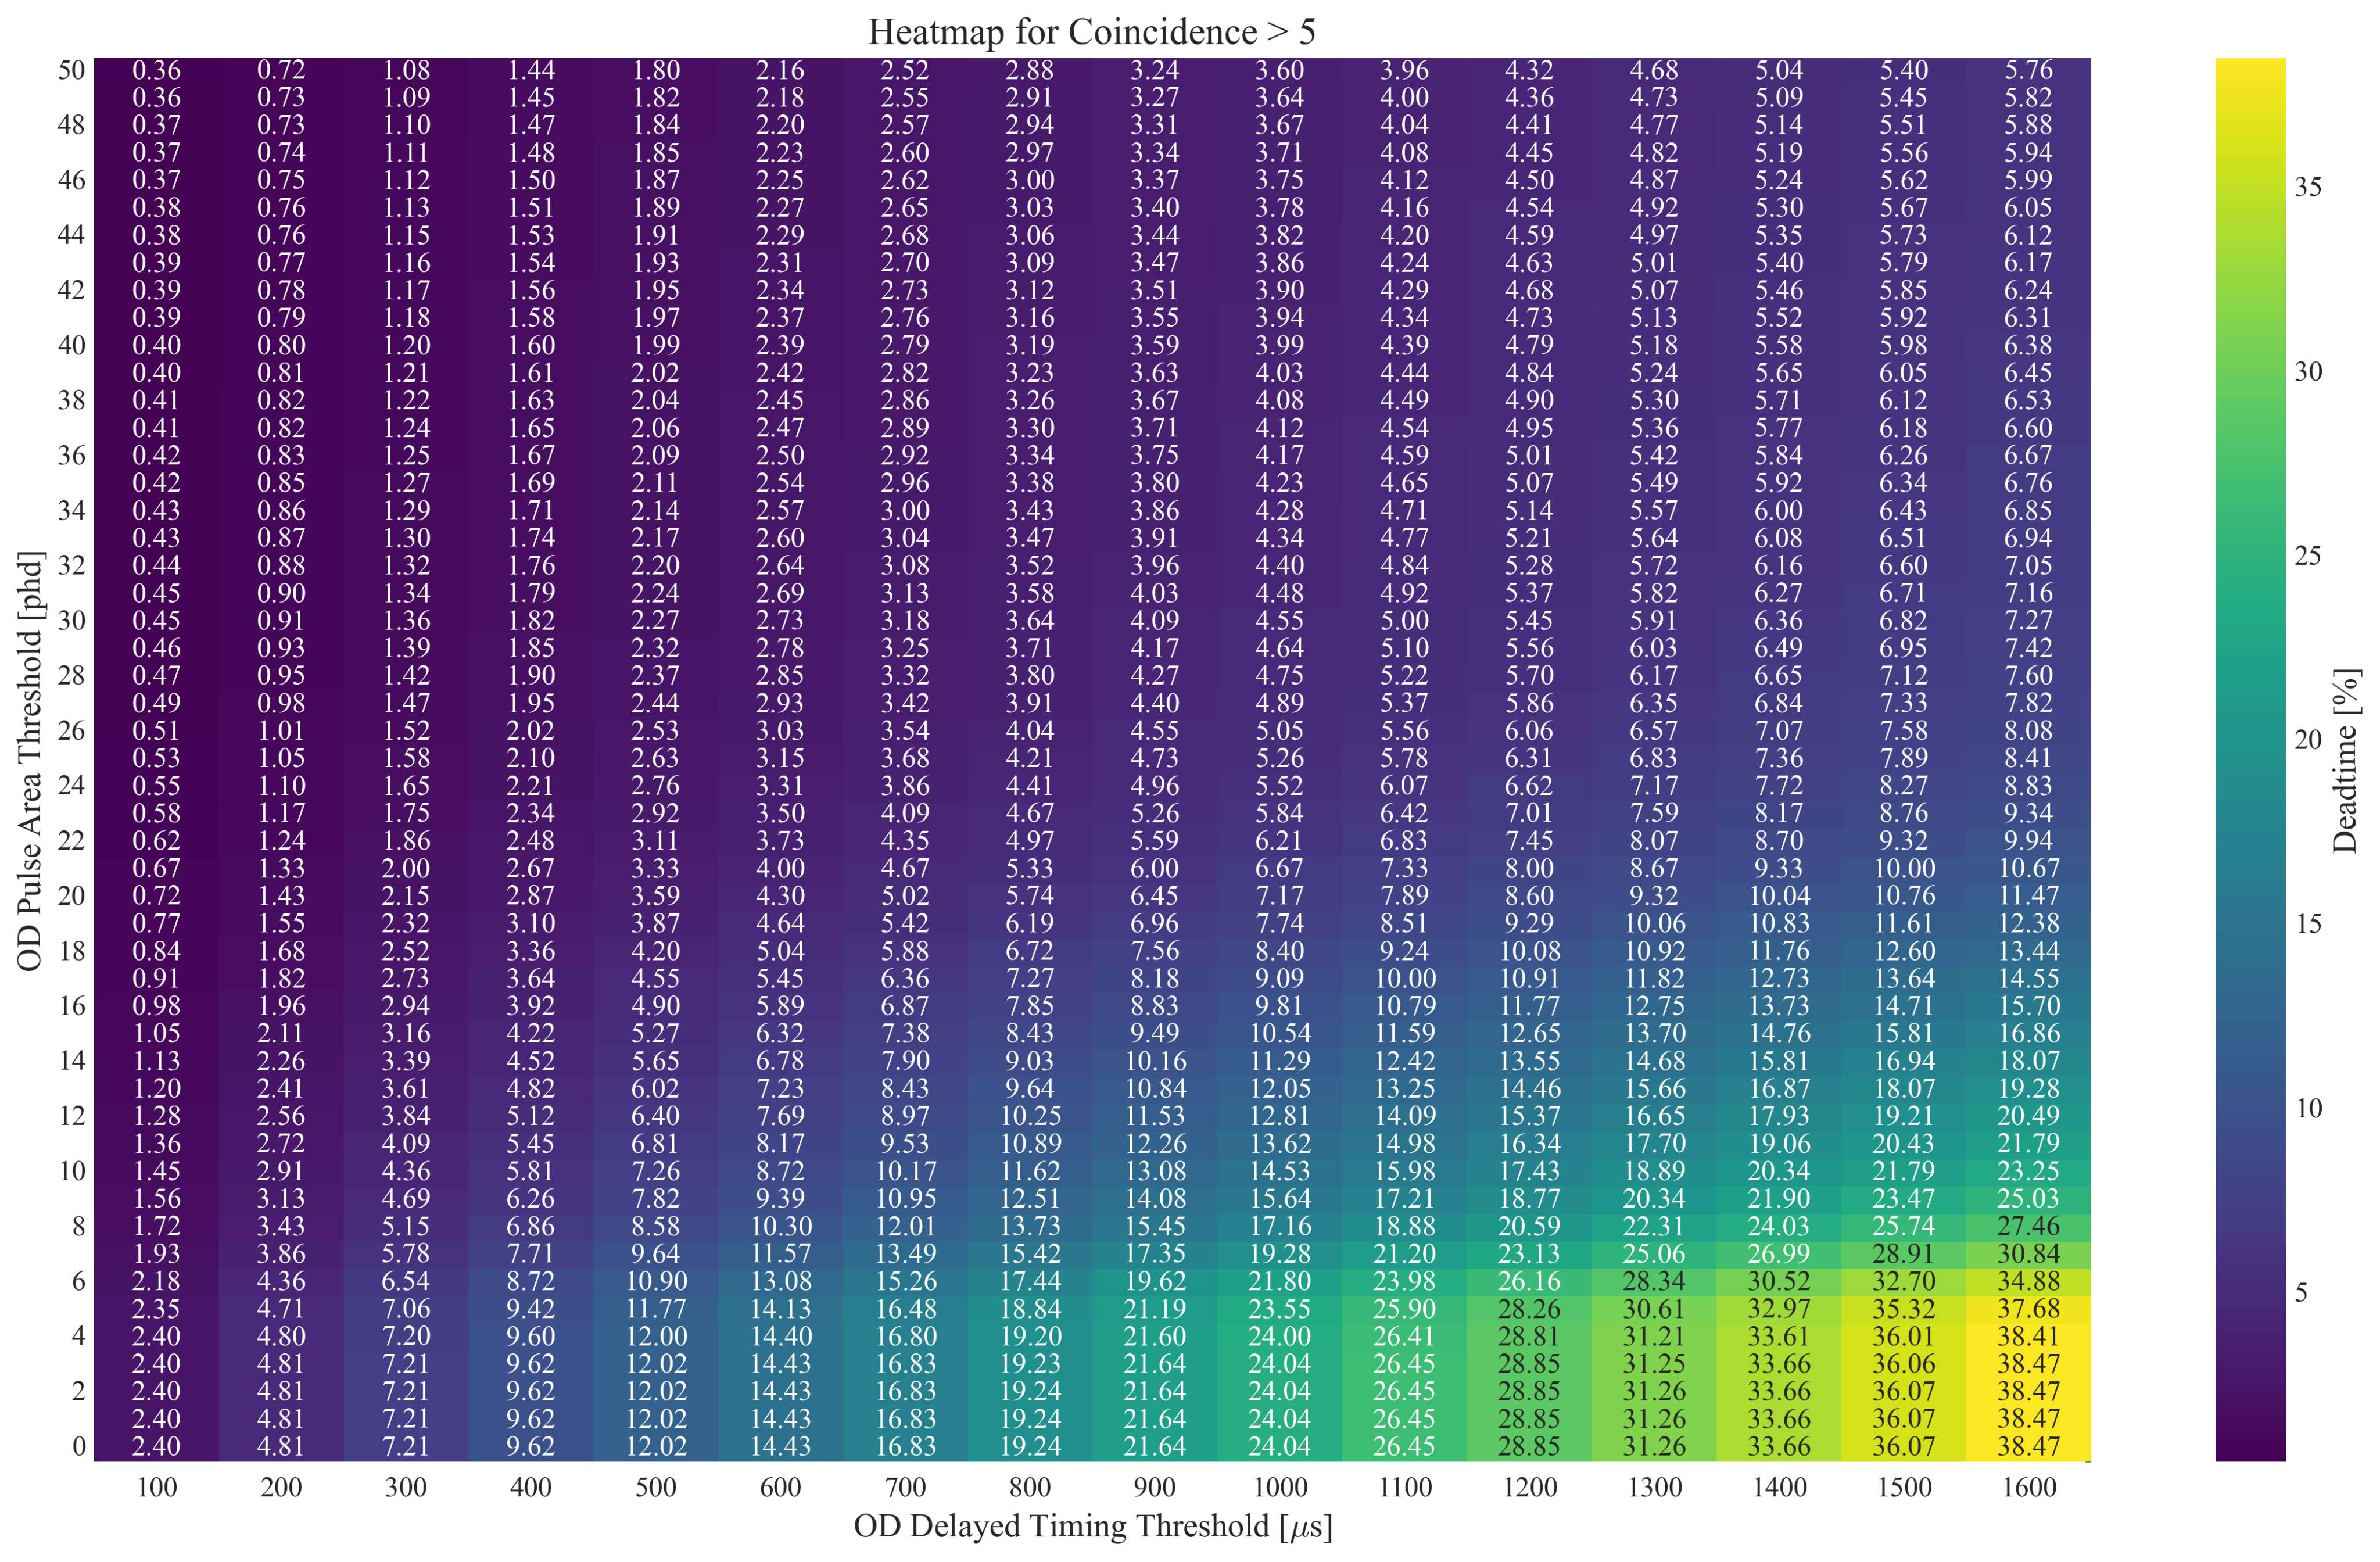
\includegraphics[width=\textwidth]{figures/VetoEfficiency/OD_Deadtime_thesis.png}
	\caption{OD Delayed heatmap.
		In each bin, either the veto window or the pulse threshold has been varied.
		The z-axis shows the deadtime associated with a given veto window and pulse threshold.
		In addition to the pulse area threshold, the pulse must have a coincidence greater than 5.}
	\label{fig:VetoEff/od_delayed_veto_heatmap}
\end{sidewaysfigure}
\begin{sidewaysfigure}
	\centering
	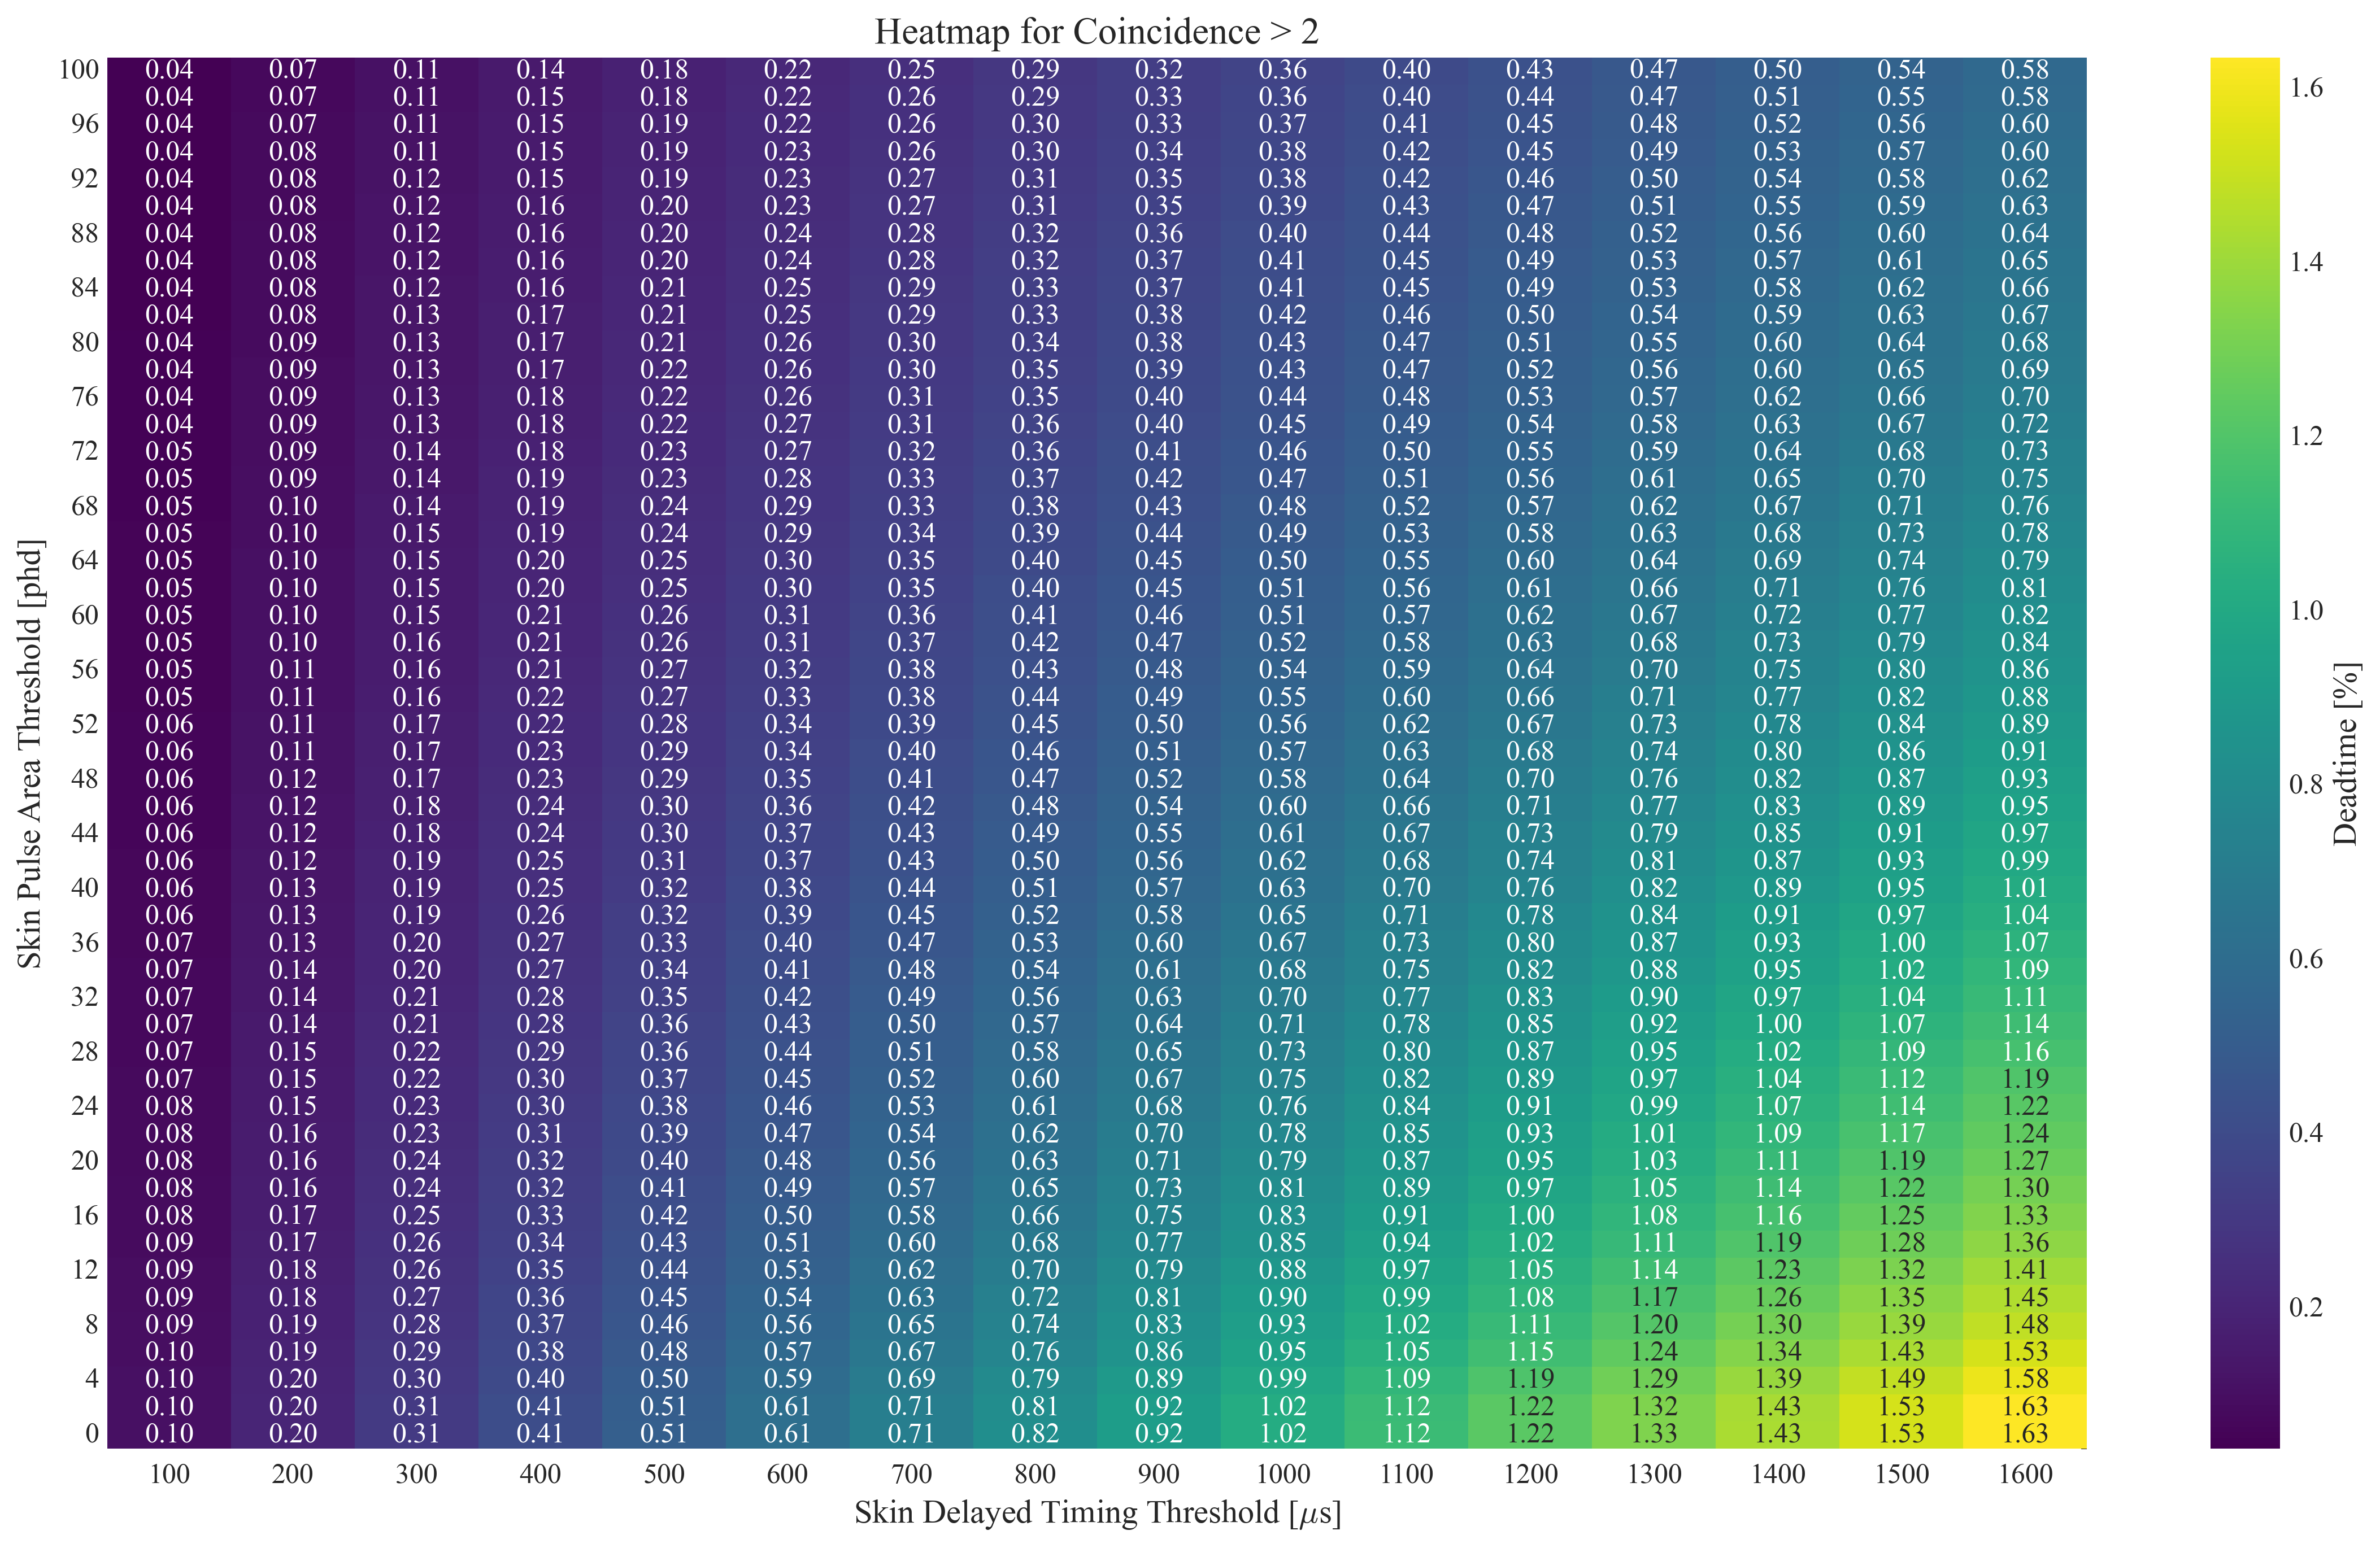
\includegraphics[width=\textwidth]{figures/VetoEfficiency/Skin_Deadtime_thesis.png}
	\caption{Delayed vetoes heatmap.
		In each bin, the OD pulse threshold or the Skin pulse threshold has been varied.
		The z-axis shows the veto efficiency associated with a given pulse thresholds.
		In addition to the pulse area threshold, the OD pulse must have a coincidence greater than 5, and the Skin pulse greater than 2.
		The veto window in this case is 500$\mu$s.}
	\label{fig:VetoEff/skin_delayed_veto_heatmap}
\end{sidewaysfigure}
\fi

\begin{figure}[!ht]
	\centering
	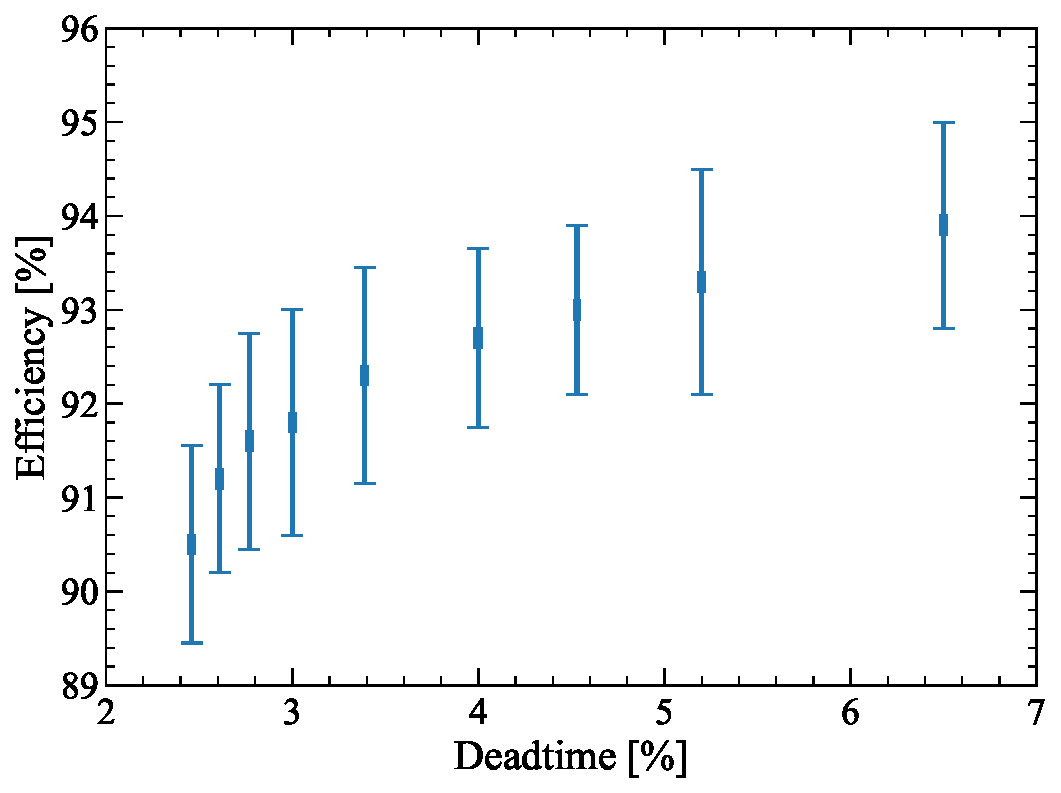
\includegraphics[width=0.6\textwidth]{figures/VetoEfficiency/DeadEffThresholdTest.pdf}
	\caption[Example plot used to highlight a number of considered cuts for the delayed Skin and OD pulse area thresholds for a 600~$\mu$s window.]{Example plot used to highlight a number of considered cuts for the delayed Skin and OD pulse area thresholds for a 600~$\mu$s window. The efficiency values have not been corrected for accidental coincidences. At each point, the numbers in brackets are the OD threshold pulse area, and the Skin threshold pulse area.}
	\label{fig:VetoEff/veto_cut_optimisation}
\end{figure}

\iffalse
\begin{figure}[!ht]
	\centering
	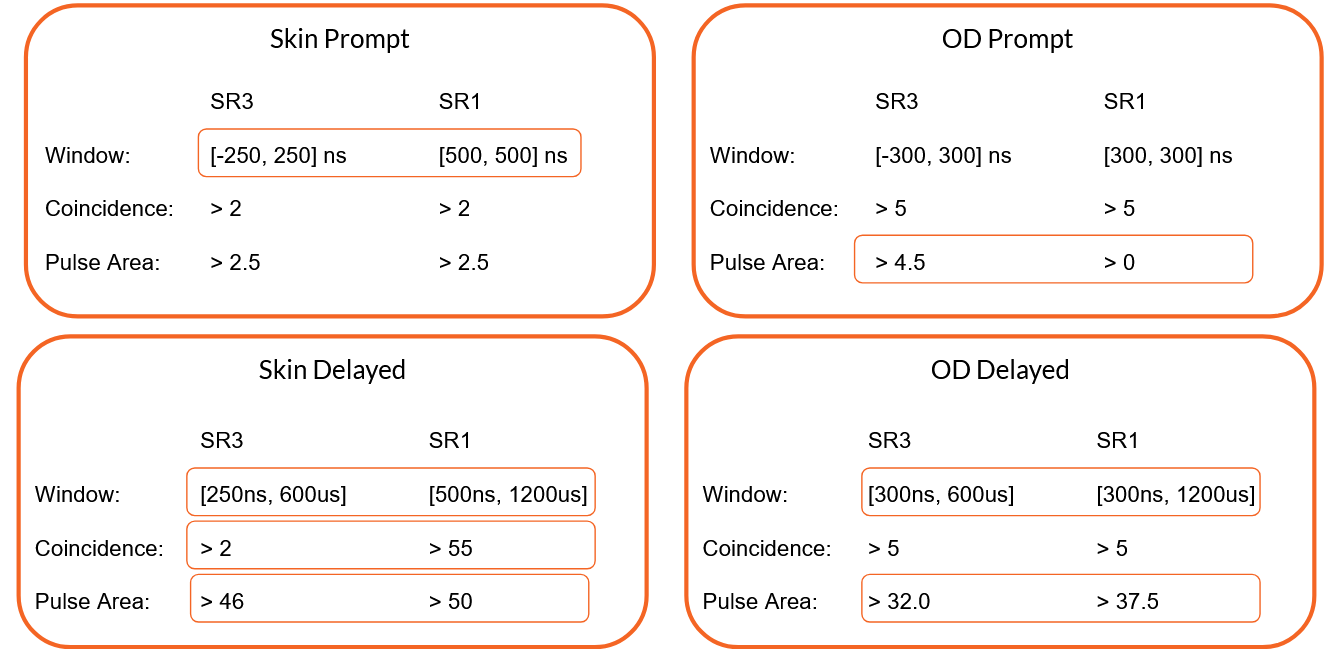
\includegraphics[width=0.9\textwidth]{figures/VetoEfficiency/sr3_cuts.png}
	\caption{Cuts determined to be optimal for the WS2024 science run.
		The WS2022 cuts are also included, where any modifications made to the selections is highlight accordingly.}
	\label{fig:VetoEff/sr3_veto_cuts}
\end{figure}
\fi

\begin{table}[!ht]
    \centering
    \caption{Cuts determined to be optimal for the WS2024 science run. The WS2022 cuts are also included, where any modifications made to the selections is highlighted accordingly.}
    \label{tab:VetoEff/sr3_veto_cuts}
    \scalebox{0.9}{
    \begin{tabular}{|c|c|c||c|c|c|}
    \hline
    \multicolumn{3}{|c||}{\textbf{Skin Prompt}} & \multicolumn{3}{c|}{\textbf{OD Prompt}} \\
    \hline
    & WS2024 & WS2022 & & WS2024 & WS2022 \\
    \hline
    Window & \cellcolor[HTML]{cecece} [-250,250]~ns & \cellcolor[HTML]{cecece}[500,500]~ns & Window & [-300,300]~ns & [-300,300]~ns\\
    Coincidence&$>2$&$>2$&Coincidence&$>5$&$>5$\\
    Pulse Area & $>2.5$ & $>2.5$ & Pulse Area & \cellcolor[HTML]{cecece}$>4.5$ &\cellcolor[HTML]{cecece} $>0$ \\    
    \hhline{|===||===|}
    \multicolumn{3}{|c||}{\textbf{Skin Delayed}} & \multicolumn{3}{c|}{\textbf{OD Delayed}} \\
    \hline
    &WS2024&WS2022&&WS2024&WS2022\\
    \hline
    Window&\cellcolor[HTML]{cecece}[250~ns, 600~$\mu$s]&\cellcolor[HTML]{cecece}[500~ns, 1200~$\mu$s]&Window&\cellcolor[HTML]{cecece}[300~ns, 600~$\mu$s]&\cellcolor[HTML]{cecece}[300~ns, 1200~$\mu$s]\\
    Coincidence&\cellcolor[HTML]{cecece}$>2$&\cellcolor[HTML]{cecece}$>55$&Coincidence&$>5$&$>5$\\
    Pulse Area&\cellcolor[HTML]{cecece}$>46$&\cellcolor[HTML]{cecece}$>50$&Pulse Area&\cellcolor[HTML]{cecece}$>32.0$&\cellcolor[HTML]{cecece}$>37.5$\\
    \hline
    \end{tabular}}
\end{table}

\subsection{Deadtime stability}\label{sec:VetoEff/DeadtimeStability}
The stability of the induced deadtime for each of the veto selection windows over the WS2024 science run was assessed for stability by comparing the deadtime at monthly intervals. For each month, the rate of pulses in the Skin and OD, using the second half of the Random Trigger data was used; and the rate above the threshold, defined by the specific veto cut, was recorded. The stability of measured deadtime over the WS2024 science run is shown in \autoref{fig:VetoEff/deadtime_stability}.
The deadtime is then calculated as:
\begin{equation}
	\textrm{Dead Time [\%]} = 100 - (\lambda(x)\cdot t_{\text{vw}})
\end{equation}
where $\lambda(x)$ is the background rate above the veto threshold $x$, and $t_{\text{vw}}$ represents the veto window length measured in ns.
The conclusion that the deadtime is stable over the WS2024 science run was confirmed by looking at the rate of OD pulses above $200~\text{keV}$ (as defined by the WS2022 energy calibration) using the \lstinline{ODHealth} PREM module. No significant fluctuation was observed during WS2024 science run, shown in \autoref{fig:VetoEff/deadtime_stability_prem}.
\begin{figure}[!ht]
	\centering
	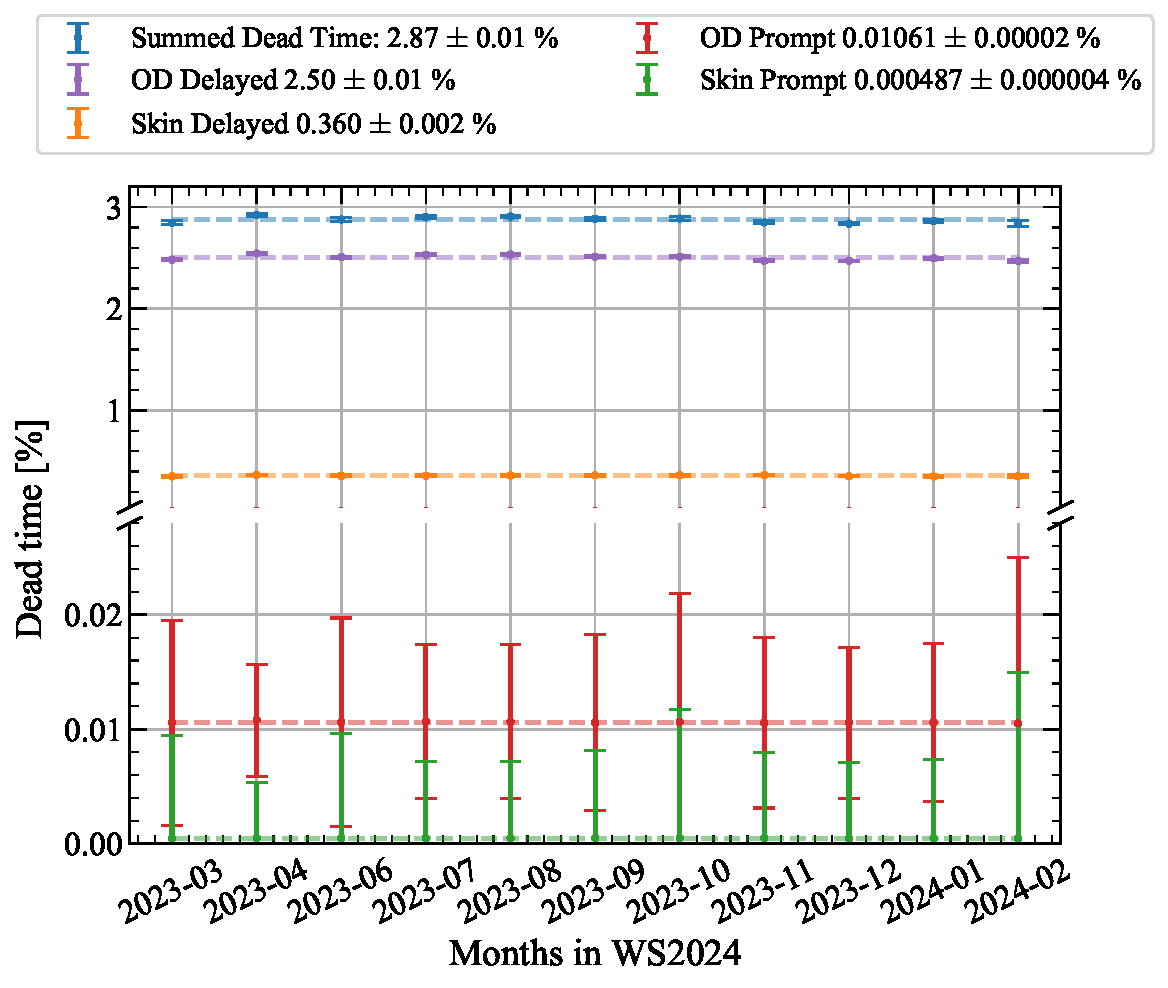
\includegraphics[width=0.7\textwidth]{figures/VetoEfficiency/SR3DeadTimeAll_withMean.pdf}
	\caption[Deadtime from the Skin and OD veto selection criteria during each month of WS2024 science run.]{Deadtime from the Skin and OD veto selection criteria during each month of WS2024 science run. The error shown in purely statistical and the mean across the science run is shown by a dashed line.}
	\label{fig:VetoEff/deadtime_stability}
\end{figure}
\begin{figure}[!ht]
	\centering
	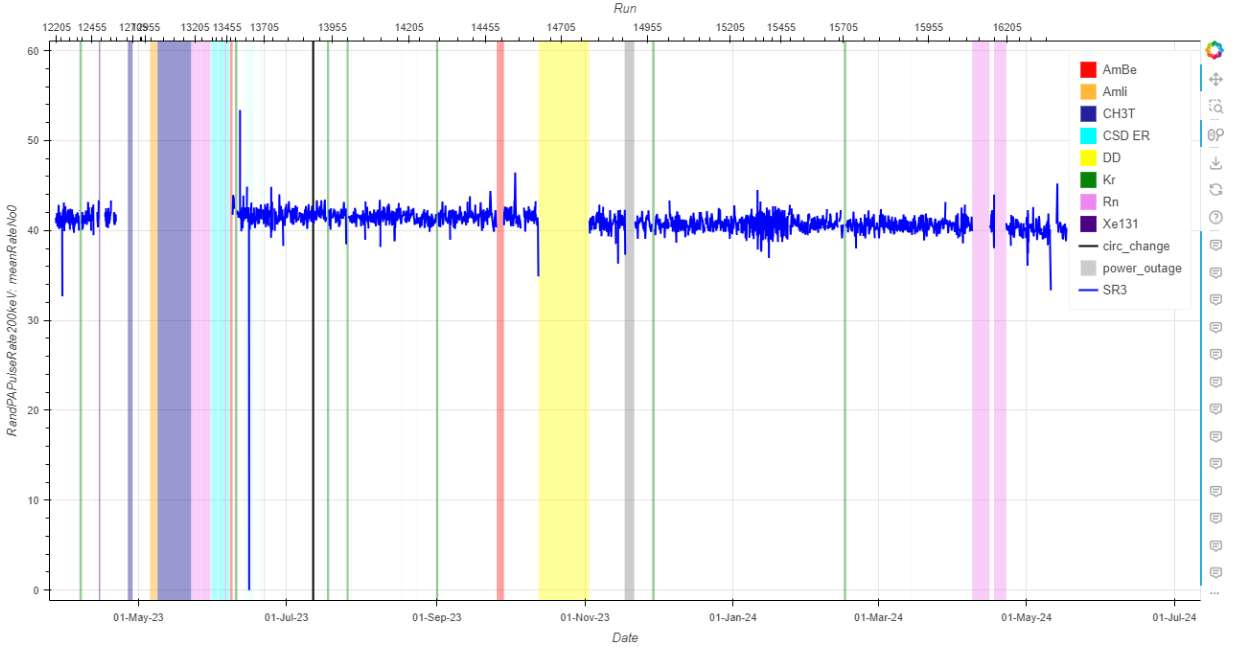
\includegraphics[width=\textwidth]{figures/VetoEfficiency/prem_od_stability.png}
	\caption{Rate of OD pulses above 200~keV (as defined by WS2022 energy calibration) over the WS2024 science run. Various periods of calibration are indicated by the coloured regions.}
	\label{fig:VetoEff/deadtime_stability_prem}
\end{figure}

\section{Neutron veto efficiency}\label{sec:VetoEff/efficiency}
In this section, the efficiency of tagging background neutrons using the Skin and OD detectors is calculated.
This is performed by calculating the efficiency on AmLi and DD calibration data and comparing to simulations.
The difference between efficiencies from simulations and data are then used to calculate an offset.
The efficiency is then calculated for Detector NR simulations and the observed offset is used as a correction factor to estimate the tagging efficiency for events classified as Detector NR \cite{LZ:2022ysc,LZ:2024zvo}.
The efficiency is defined as:
\begin{equation}\label{eqn:VetoEff/:neutron_tagging_efficiency}
	\epsilon [\%] = \frac{\textrm{N. Events passing Analysis Cuts + Veto Cuts}}{\textrm{N. Events passing Analysis Cuts}} \times 100
\end{equation}
and the inefficiency is defined as $100 - \epsilon$.

\subsection{Neutrons from calibration sources \label{sec:VetoEff/AmLi_Efficiency}}
\subsubsection{AmLi}
AmLi calibration data used is this study was taken during May 2023 calibration campaign prior to the WS2024 science run. Events which were classified as single scatters by LZap and passed the selection outlined in \ref{tab:VetoEff/amli_efficiency_cuts} were used for the study. Two additional cuts were applied to the calibration data:
\begin{enumerate}
	\item \textbf{CSD tube position selection}: A circular cut on the reconstructed position of the SS in the TPC such that events from just one CSD tube are selected at a time. During the calibration campaign, sources were simultaneously deployed in each of the CSD tubes at equal heights (three separate height positions were used, $z=100~\text{mm},700~\text{mm},1300~\text{mm}$ relative to cathode at $z=0~\text{mm}$). Whereas separate simulations were produced with a single source in each CSD tube at three different heights (equal to $z$-position used in the calibration campaign). 
    The circular cut selects events within a 50~mm radius of the CSD tube. The boundaries for each of the cuts respective to the individual CSD tubes is shown in \autoref{fig:VetoEff/CSDSelection}. 
    \begin{figure}[!ht]
    \centering
        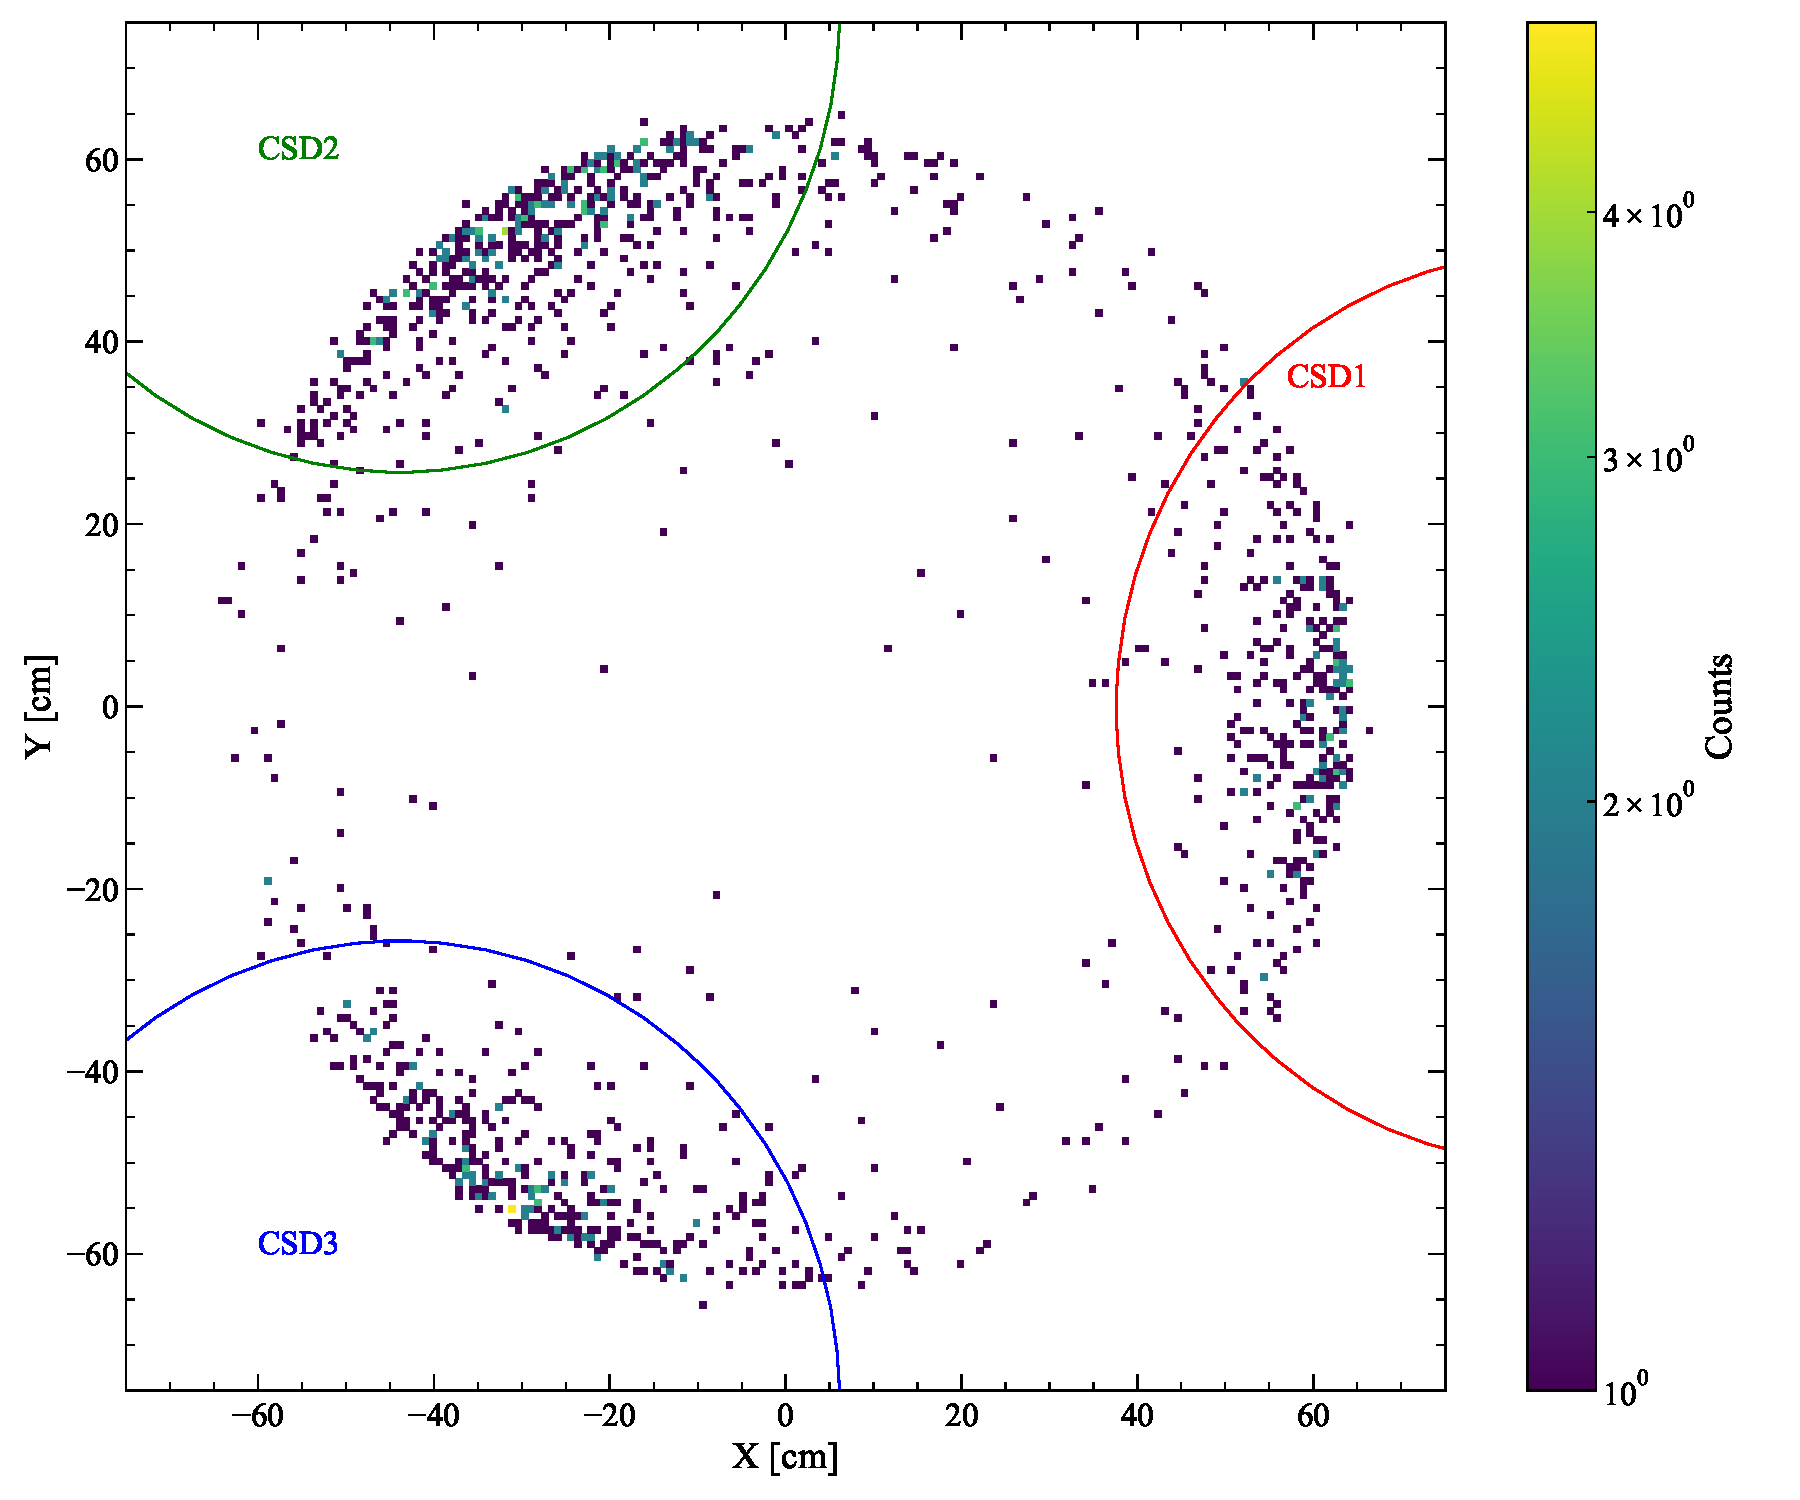
\includegraphics[width=0.7\textwidth]{figures/VetoEfficiency/CircularCSDCut.pdf}
        \caption{X-Y distribution of events in the TPC for AmLi sources positioned at 700mm. Each of the circular cuts are overlaid onto the plot.}
        \label{fig:VetoEff/CSDSelection}
    \end{figure}
    The position dependence of the veto efficiency can be examined by applying the CSD tube selection to data collected at different $z$-positions. The veto efficiency for different CSD tubes and $z$-positions is shown in \autoref{fig:VetoEff/VetoEffPositionDependence}.
    \begin{figure}[!ht]
    	\centering
    	\begin{subfigure}[b]{0.48\textwidth}
    		\centering
    		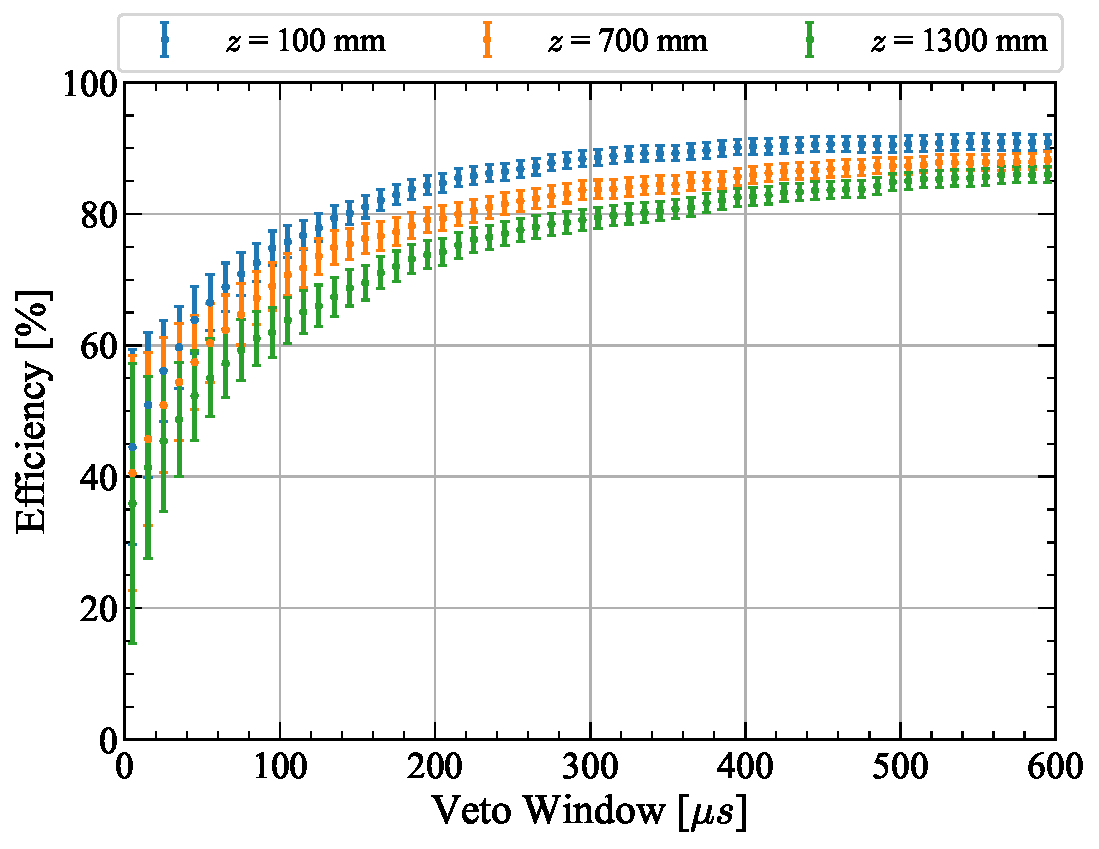
\includegraphics[width=\textwidth]{figures/VetoEfficiency/Eff_AmLi_Total_AllHeights.pdf}
            \caption{}
    		\label{fig:VetoEff/VetoEffPositionDependenceCSD}
    	\end{subfigure}
    	\hfill
    	\begin{subfigure}[b]{0.48\textwidth}
    		\centering
    		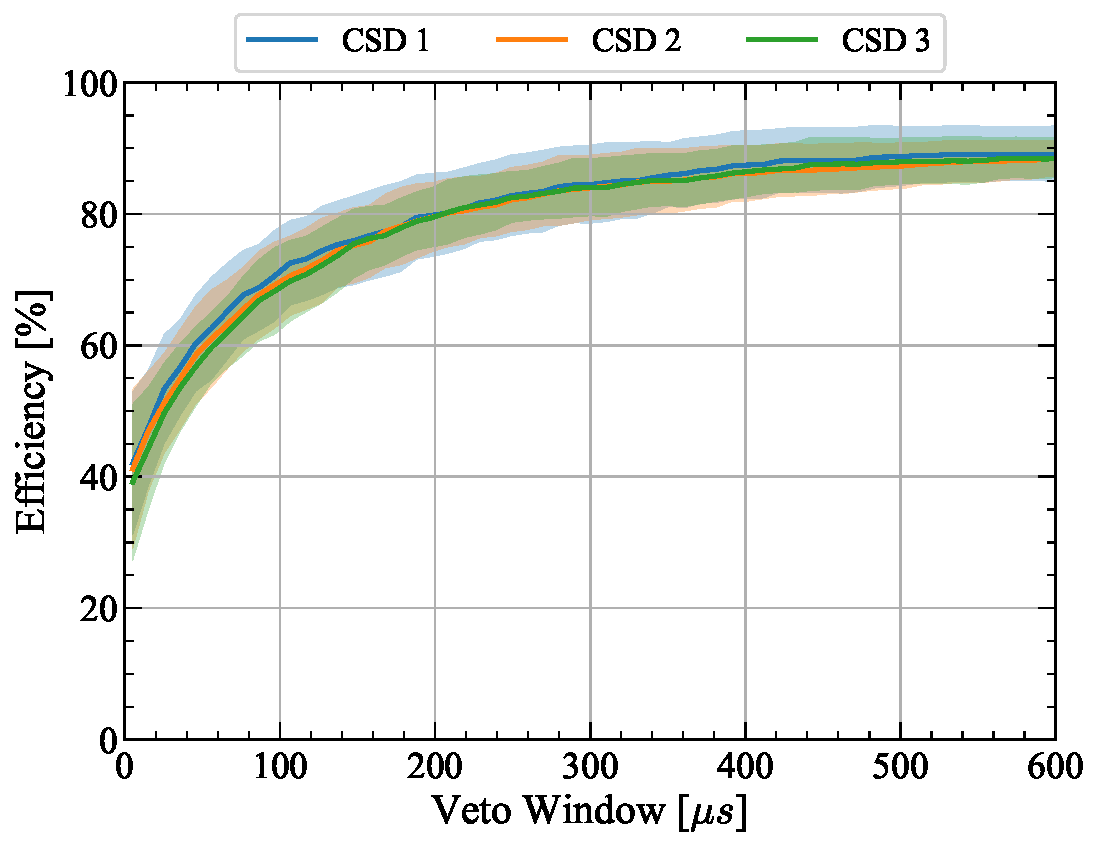
\includegraphics[width=\textwidth]{figures/VetoEfficiency/Eff_AmLi_Total_AllCSD.pdf}
    		\caption{}
            \label{fig:VetoEff/VetoEffPositionDependenceZPos}
    	\end{subfigure}
    	\caption{Position dependent veto efficiencies for different $z$ (left) and CSD positions (right).}
    	\label{fig:VetoEff/VetoEffPositionDependence}
    \end{figure}
	A concern of this cut is that events towards the centre of the TPC are excluded. When the efficiency is averaged across different heights and CSD tube, the average can then be replicated in both data and simulation. 
    The position-averaged efficiency when the CSD cut is applied is $(88.21\pm1.03)\%$, whereas without the cut, the efficiency is $(88.25\pm1.22)\%$.
	Across the $600~\mu s$ window, there is no greater than $2\%$ difference between when the cut is and isn't applied.
	This comparison is shown in \autoref{fig:VetoEff/CSDSelectionEffComp}.
    \begin{figure}[!ht]
    	\centering
    	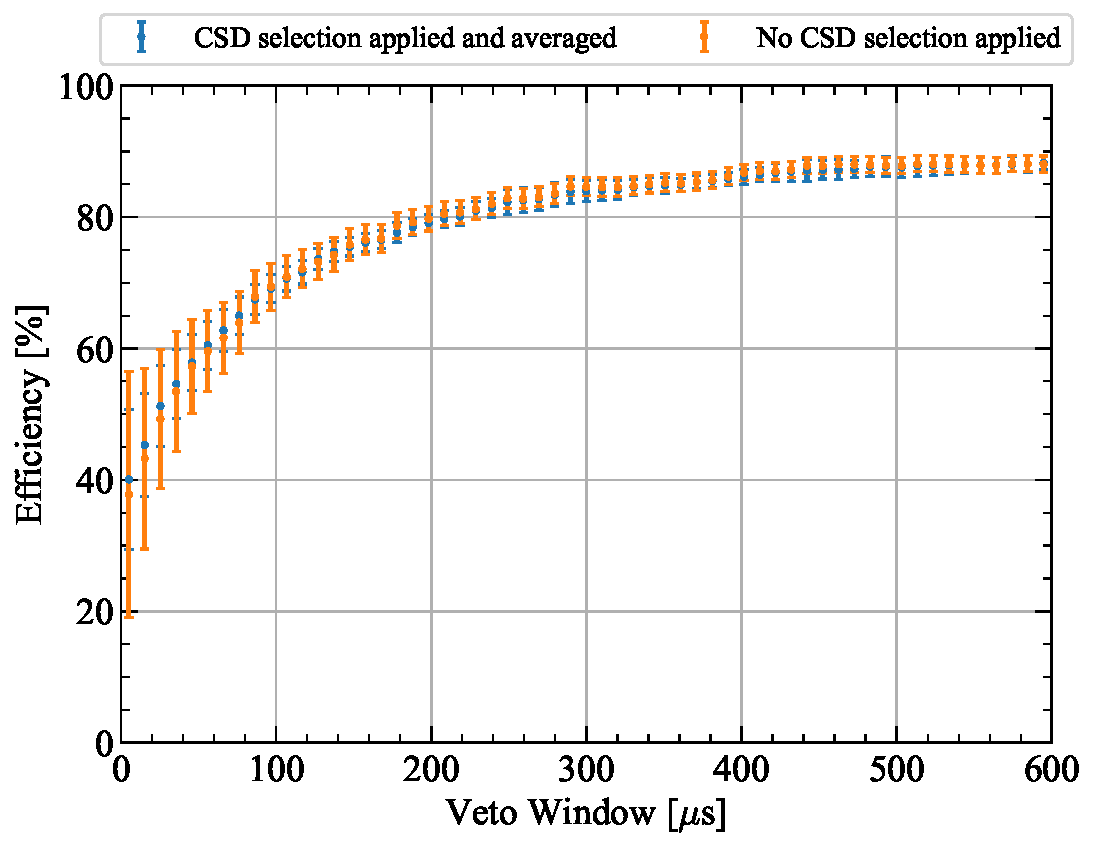
\includegraphics[width=0.7\linewidth]{figures/VetoEfficiency/CSDSelectionCheck.pdf}
    	\caption[CSD tube selection impact on veto efficiency.]{CSD tube selection impact on veto efficiency. The average veto efficiency for events which have a reconstructed position with 50~mm of a CSD tube (blue) is compared to veto efficiency of all events with no CSD selection applied. The cut has $<5\%$ impact across the veto window and $<0.1\%$ impact at the 600~$\mu$s veto window threshold.}
    	\label{fig:VetoEff/CSDSelectionEffComp}
    \end{figure}

	\item \textbf{NR-band selection}: Events which lie within 1-$\sigma$ of NR band median are selected to be used in the veto efficiency calculation. The purpose of this cut is to improve the purity of the selection. The NR bands are generated using the Noble Element Simulation Technique (NEST) \cite{NEST2011} are shown in \autoref{fig:VetoEff/SR3NRBands}.
    \begin{figure}[!ht]
    	\centering
    	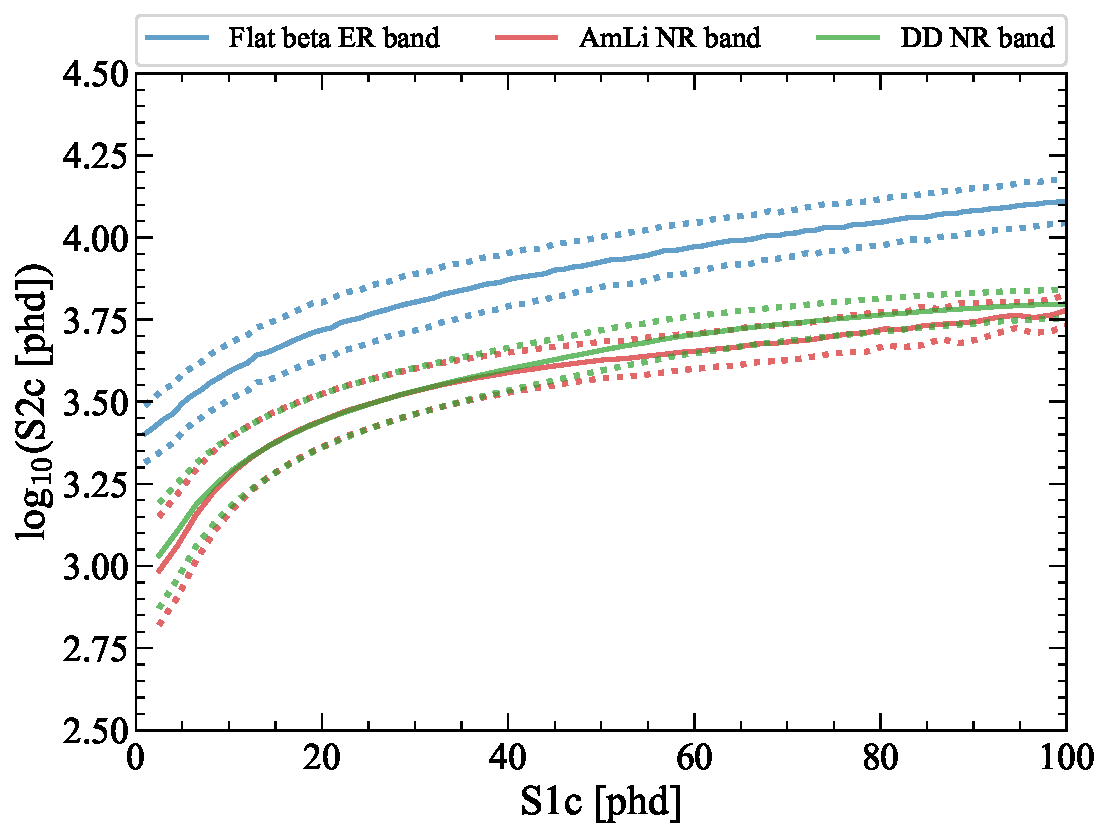
\includegraphics[width=0.7\textwidth]{figures/VetoEfficiency/NRBands.pdf}
    	\caption{The NR band medians with 1-$\sigma$ boundaries for AmLi and DD calibration sources. Both NR bands and 1-$\sigma$ boundaries were generated using NEST.}
    	\label{fig:VetoEff/SR3NRBands}
    \end{figure}
\end{enumerate}


\subsubsection{AmLi accidental correction}\label{sec:VetoEff/AmLiAccCorrection}
When determining the veto tagging efficiency a correction must be applied to the measured efficiency to account for the accidental coincidences from AmLi gammas (and neutrons) with single scatter nuclear recoils in the TPC which can artificially enhance the measured tagging efficiency.
First, veto inefficiency must be defined. Every time a single scatter nuclear recoil is observed in the TPC, a veto window is opened, this can be recorded using a counter, $N$ every time this happens.
If there is no pulse observed in the Skin or the OD that satisfies the veto requirements, this event is not vetoed and recorded using a counter, $M$. Resulting in a total inefficiency, $M/N$, and a total efficiency, $1-M/N$.
The effect of the accidentals be a result of the following process.
If a neutron enters the TPC, scatters and is not detected by the vetos, the counter $M$ should be iterated but there is an accidental coincidence of a gamma or a neutron from the AmLi sources with the TPC scatter so the count is not iterated.
The probability of this happening can be written as $1-P_a(0)$, where $P_a(0)$ is the probability of seeing zero accidental pulses in the Skin and OD coincidence windows.
Using probability and the counters, the true inefficiency is described below,
\begin{gather*}
	M_{observed}=M_{true}-M_{true}(1-P_a(0)) \\
	M_{observed}=M_{true}P_a(0)\rightarrow M_{true}=M_{observed}/P_a(0)\\
	Ineff_{true}=M_{true}/N\;and\;Ineff_{observed}=M_{observed}/N\\
	\Rightarrow Ineff_{true}=Ineff_{observed}/P_a(0)
\end{gather*}
Due to the logic of the inefficiency calculation is that the $M$ counter iterates in an AND condition such that all coincidence windows in all detector have to be empty.
This leads to a final inefficiency of,
\begin{equation}
	Ineff_{true} = Ineff_{obs}  / (1 - P_a(>0)_{any\:window})
\end{equation}
$P_a(>0)_{any\:window}$ can be determined directly using the post-trigger window of randomly triggered events (GPS events) and count any pulses in \textbf{any} of the veto detectors.
The accidental correction is correlated with the length of the veto window, scans over the entire delayed veto window in 10$\mu$s steps, the change in the correction factor over time can be seen in \autoref{fig:VetoEff/AccCorr}.
The impact of the accidental correction when applied to the efficiency can be seen in \autoref{fig:VetoEff/AccidentalImpact}.
\begin{figure}[!ht]
	\centering
	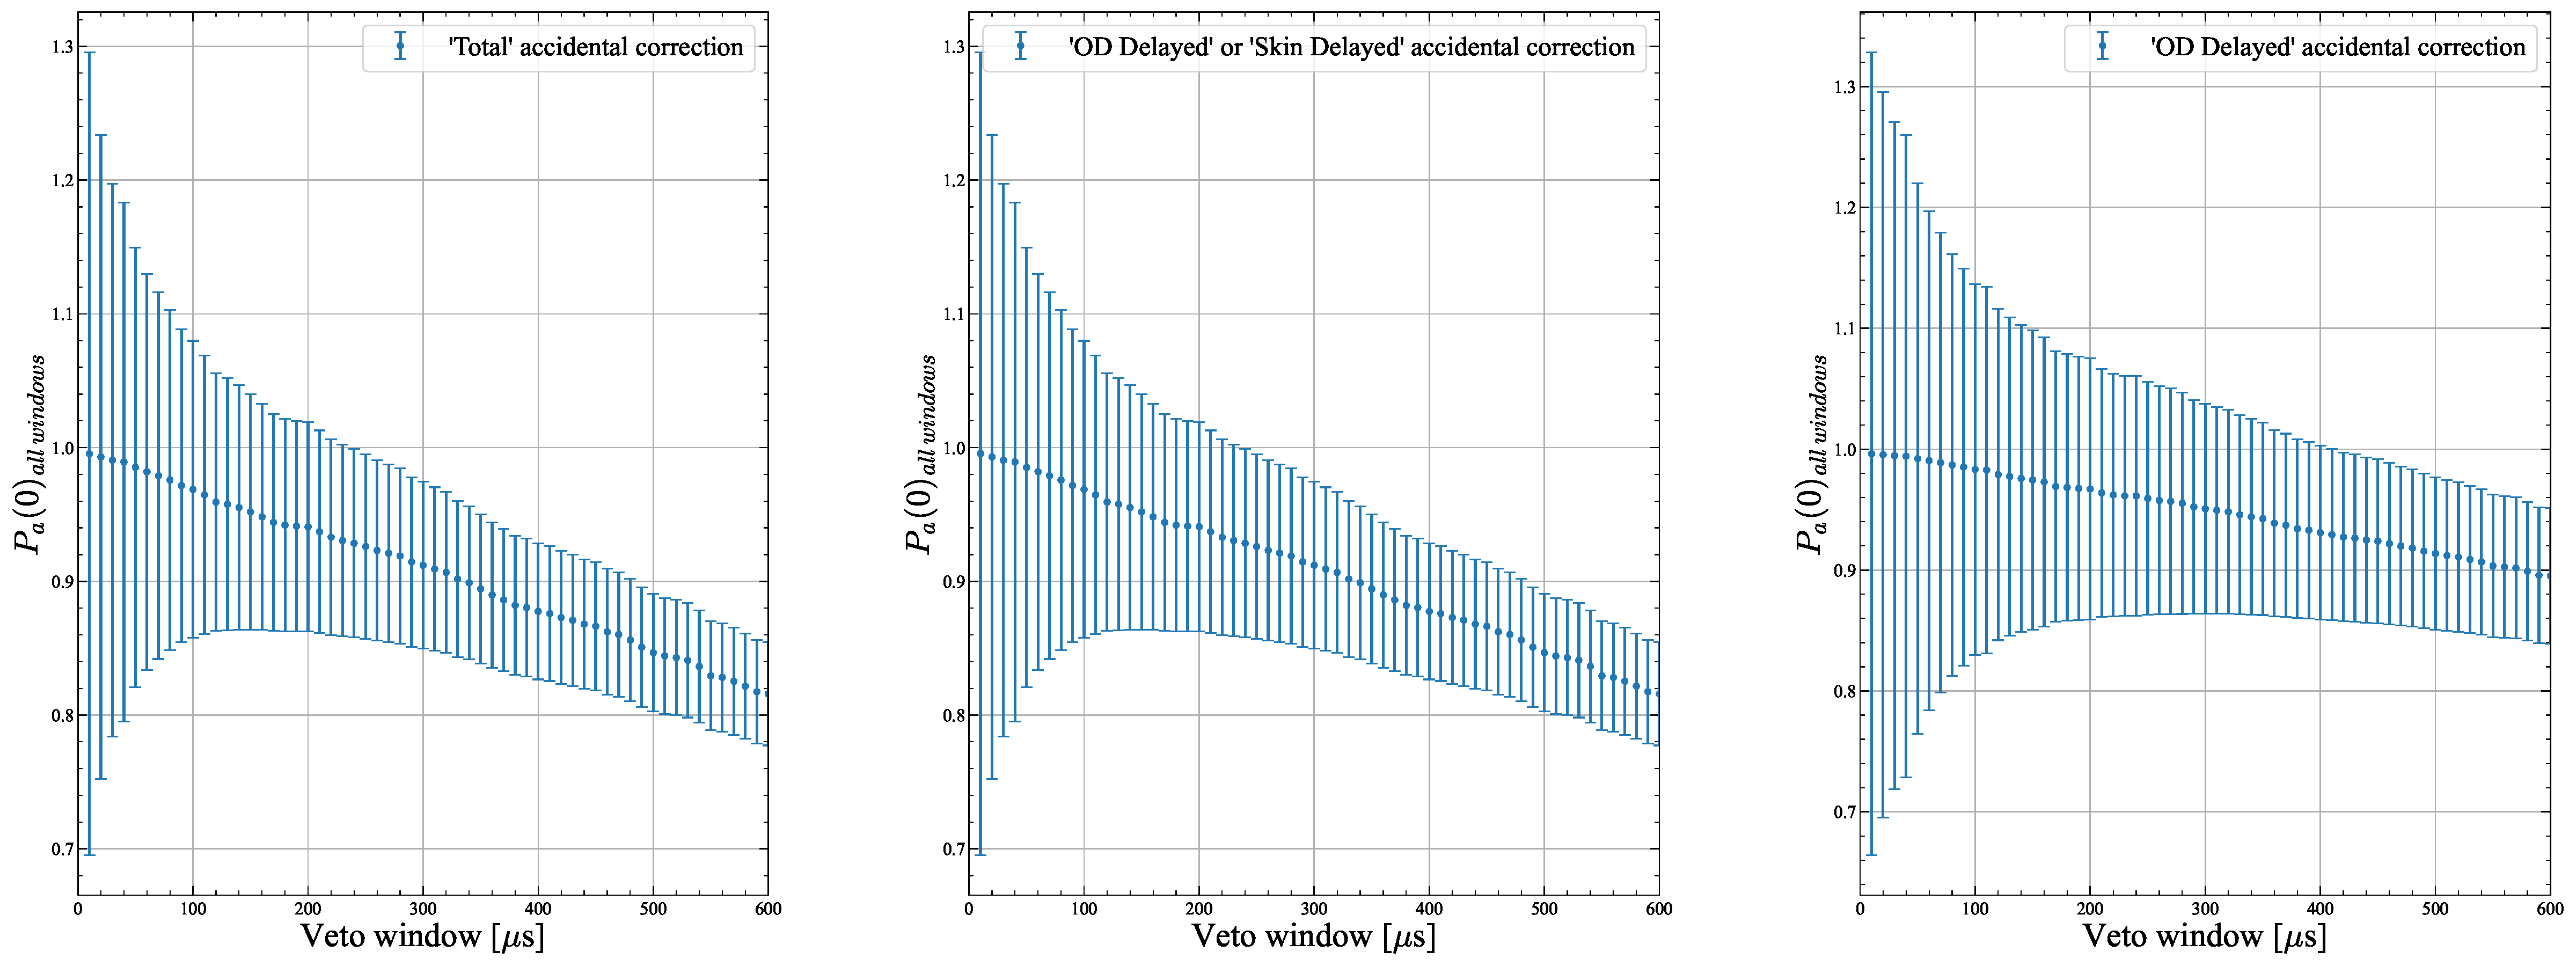
\includegraphics[width=\textwidth]{figures/VetoEfficiency/SR3AmLi_700_Corrections_100k_P0.pdf}
	\caption{$P_a(>0)_{all\:window}$ AmLi Accidental correction factors for varying veto window size for different windows of interest.}
	\label{fig:VetoEff/AccCorr}
\end{figure}
\begin{figure}[!ht]
	\centering
	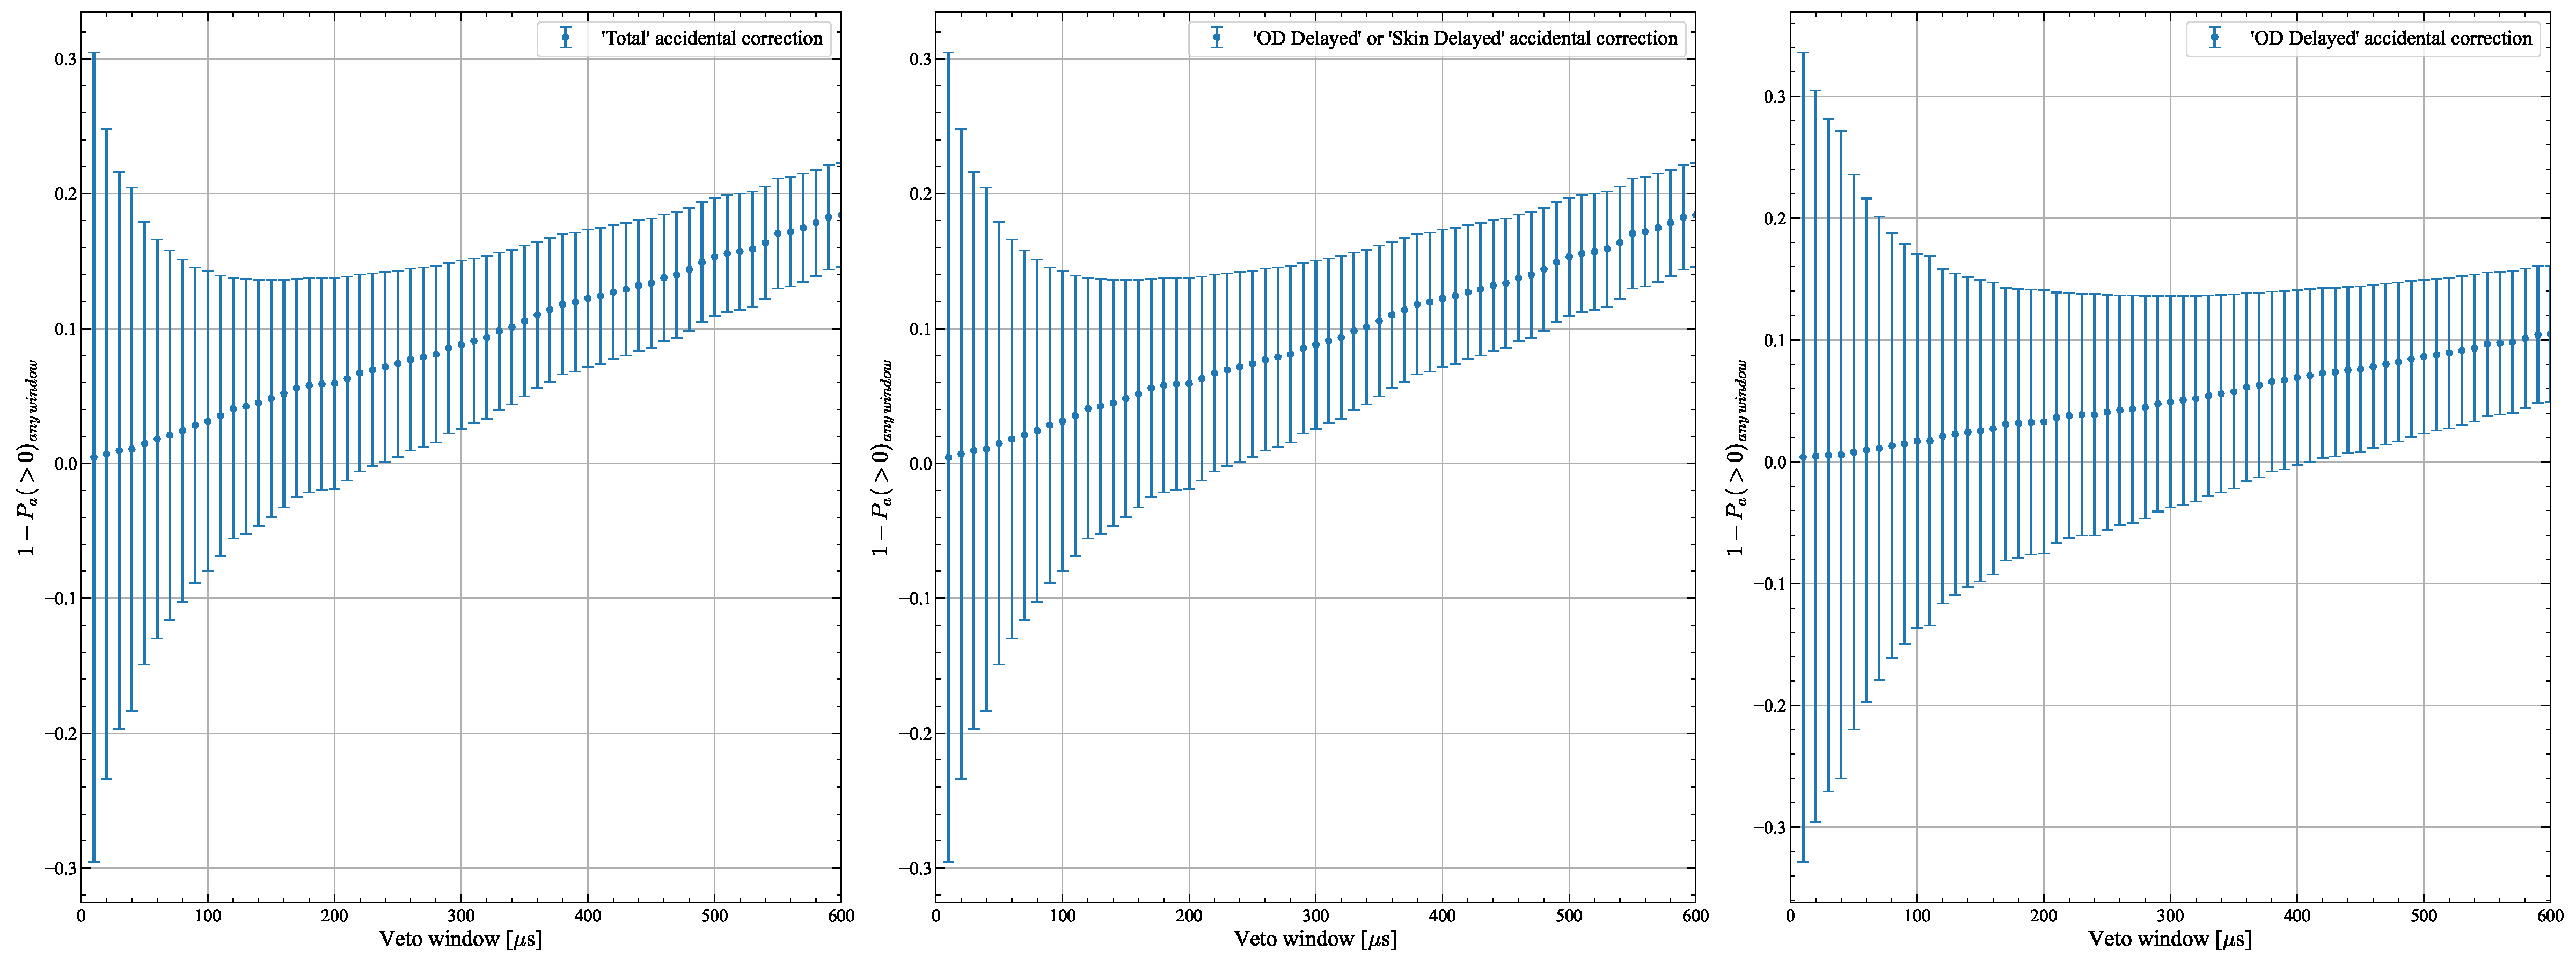
\includegraphics[width=\textwidth]{figures/VetoEfficiency/SR3AmLi_700_Corrections_100k_P0-1.pdf}
	\caption{$1 - P_a(>0)_{any window}$ AmLi Accidental correction factors for varying veto window size for different windows of interest.}
	\label{fig:VetoEff/AccCorr_P0-1}
\end{figure}
\begin{figure}[!ht]
	\centering
	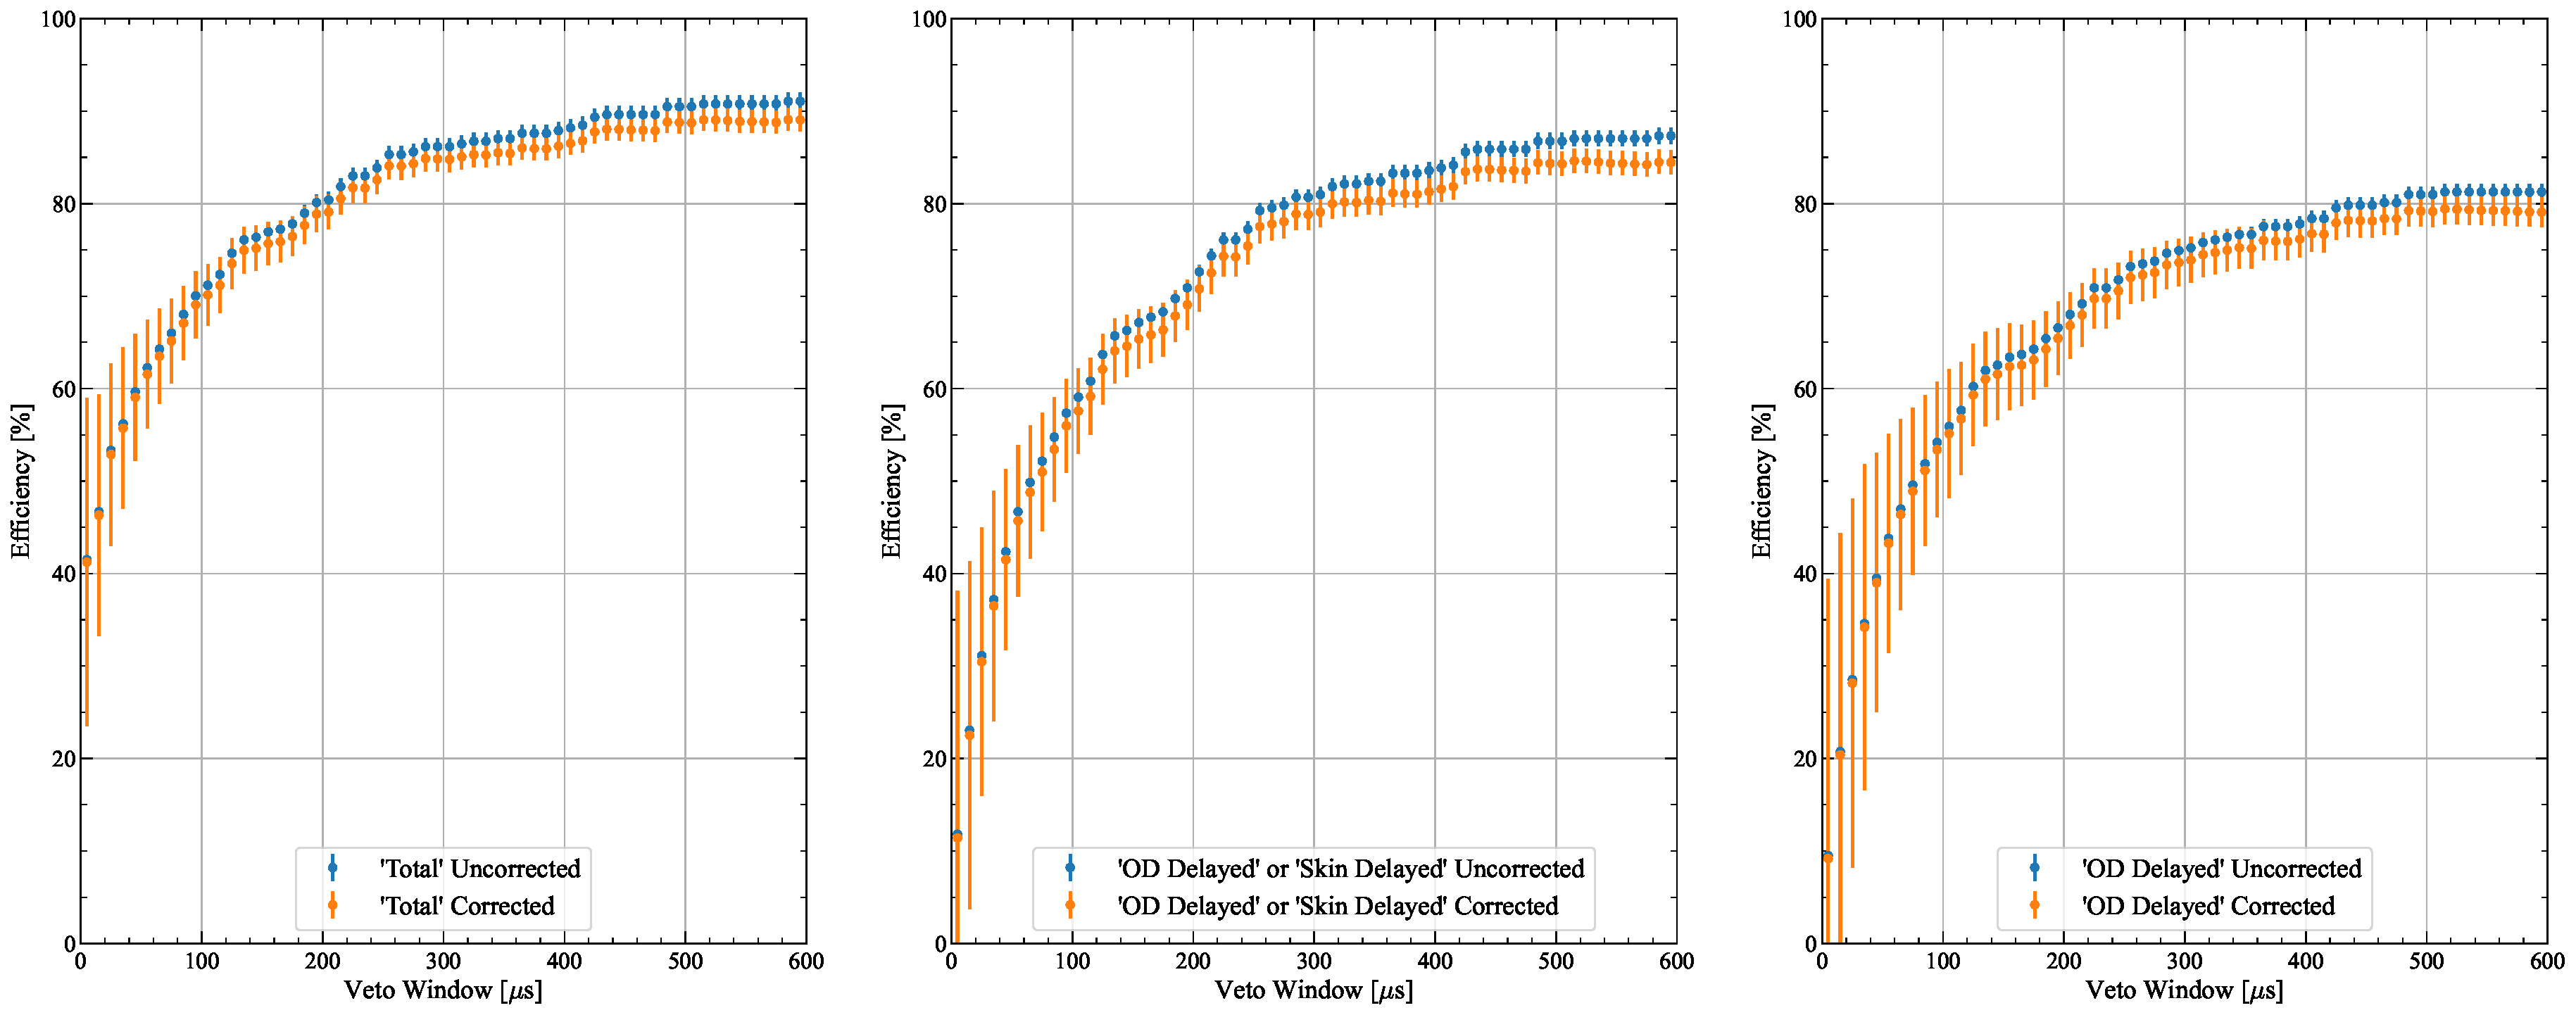
\includegraphics[width=\textwidth]{figures/VetoEfficiency/AccidentalCorrectionImpact.pdf}
	\caption{The impact of the accidental correction applied to the different veto efficiencies for the given windows of interest. AmLi data at a height of 700~mm in CSD1 has been used here as an example.}
	\label{fig:VetoEff/AccidentalImpact}
\end{figure}


\subsubsection{DD direct}
The DD calibration runs are from the October-2023 calibration period during the WS2024 science run, with run control operation name \textbf{DD Plasma}.
The runs used are; \lstinline{14631-14654}.
All files were processed with \lstinline{LZAP-5.8.0}.
The analysis for DD follows a logic similar to the AmLi described in \autoref{sec:VetoEff/AmLi_Efficiency}.
The cuts used for DD are listed in \autoref{tab:VetoEff/dd_efficiency_cuts}.
In addition to these cuts, an NR band cut was also applied.
It is important to note that this NR band is different to the one used for AmLi. The two different NR bands for the calibration sources is shown in \autoref{fig:VetoEff/SR3NRBands}.
%The band can be found on NERSC at \lstinline{/global/cfs/cdirs/lz/physics/NEST_Bands/SR3/20240313/Calibration}, if it has been moved, it can be recreated with the Woods parameters listed below;
The band was generated using the NEST, it can be recreated with the Woods parameters listed below;
\begin{lstlisting}[backgroundcolor = \color{lightgray}]
The Woods Function Fit Parameters for the Band Mean are:
[-19.937161961102728, 19.923601138859933,
0.0003111152850489644, 3.9306761416517557]

The Woods Function Fit Parameters for the 10% CL Line are:
[-17.635537023159518, 15.192184130700792,
0.000791717641575967, 3.813184578175848]

The Woods Function Fit Parameters for the 90% CL Line are:
[-32.02840007751605, 32.68367426603315,
-0.0006477294838326959, 4.157363202993382]
\end{lstlisting}
\begin{table}[!ht]
	\centering
	\caption{ALPACA-Core WS2024 cuts used on DD calibration data for determining the efficiency.}
	\begin{tabular}{lll}
    \hline\hline
	\textbf{Physics cuts}&\textbf{ S1 cuts}&\textbf{S2 cuts} \\
	\hline
	Single scatter & S2 width vs drift time & S1 prominence cut \\
	S1 and S2 threshold & Narrow S2 & Stinger event cut \\
	Fiducial Volume & S2 rise time & S1 TBA vs drift time \\
	& S2 early peak & S1 HSC cut \\
	& S2 XY quality & S1 shape \\
	& S2 TBA (above-anode gas) & S1 photon timing \\
    \hline\hline
	\end{tabular}
	\label{tab:VetoEff/dd_efficiency_cuts}
\end{table}
\subsubsection{DD accidental correction}
The DD calibration data was also corrected for accidentals. The same method was used which was previously discussed in \autoref{sec:VetoEff/AmLiAccCorrection}. The correction factors used as a function of veto window can be seen in \autoref{fig:VetoEff/DDAccCorrectionParameters}.
The impact of the accidental corrections on the DD veto efficiency can be seen in \autoref{fig:VetoEff/DDAccCorrectionImpact_P0}.

\begin{figure}[!ht]
	\centering
	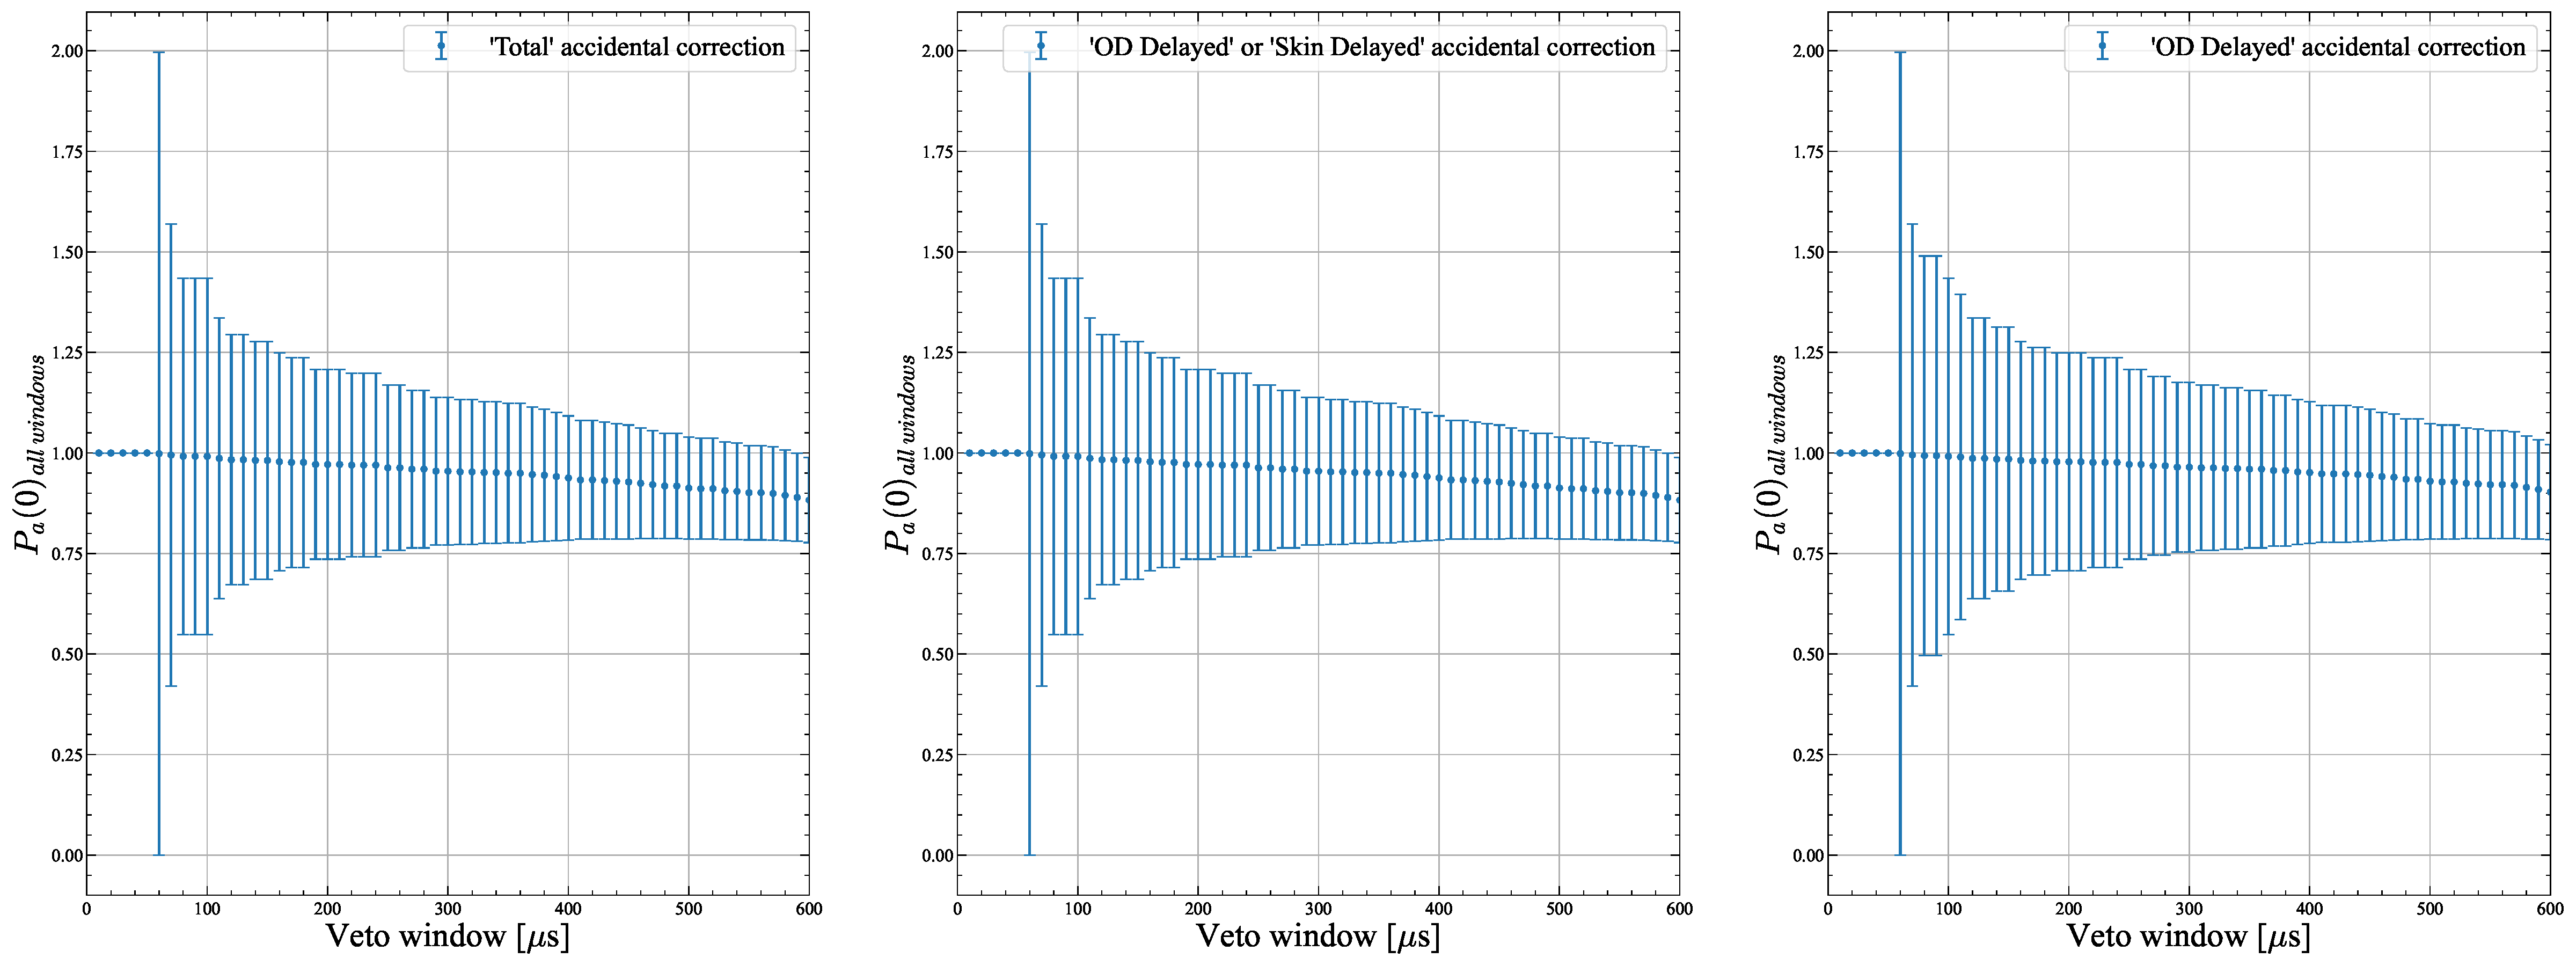
\includegraphics[width=\textwidth]{figures/VetoEfficiency/DDAccCorrectionImpact_P0.pdf}
	\caption{$P_a(>0)_{all\:window}$ DD Accidental correction factors for varying veto window size for different windows of interest.}
	\label{fig:VetoEff/DDAccCorrectionImpact_P0}
\end{figure}

\begin{figure}[!ht]
	\centering
	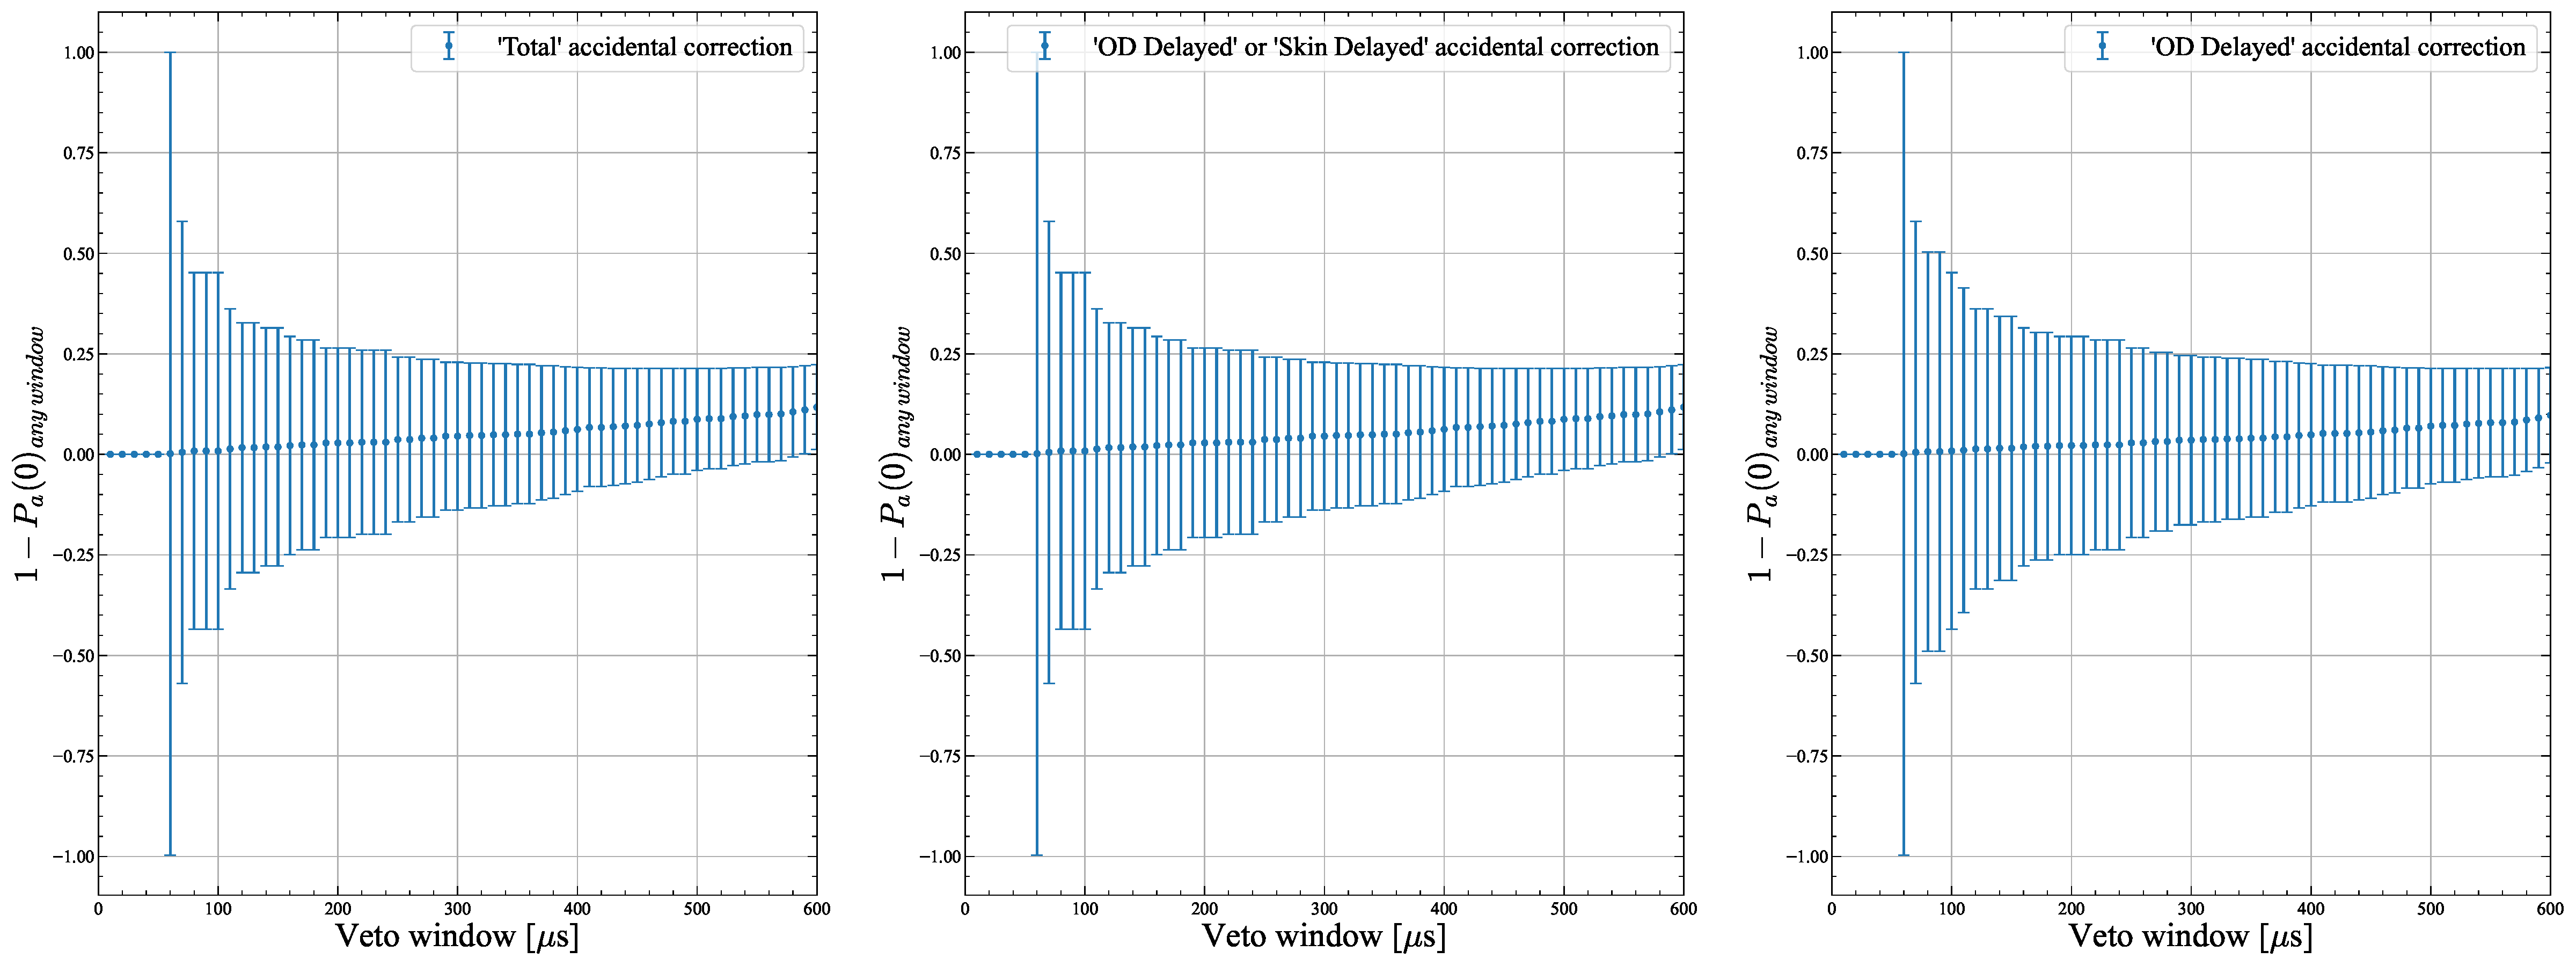
\includegraphics[width=\textwidth]{figures/VetoEfficiency/DDAccCorrectionImpact_1-P0.pdf}
	\caption{$1-P_a(>0)_{any\:window}$DD Accidental correction factors for varying veto window size for different windows of interest.}
	\label{fig:VetoEff/DDAccCorrectionImpact_1-P0}
\end{figure}

\begin{figure}[!ht]
	\centering
	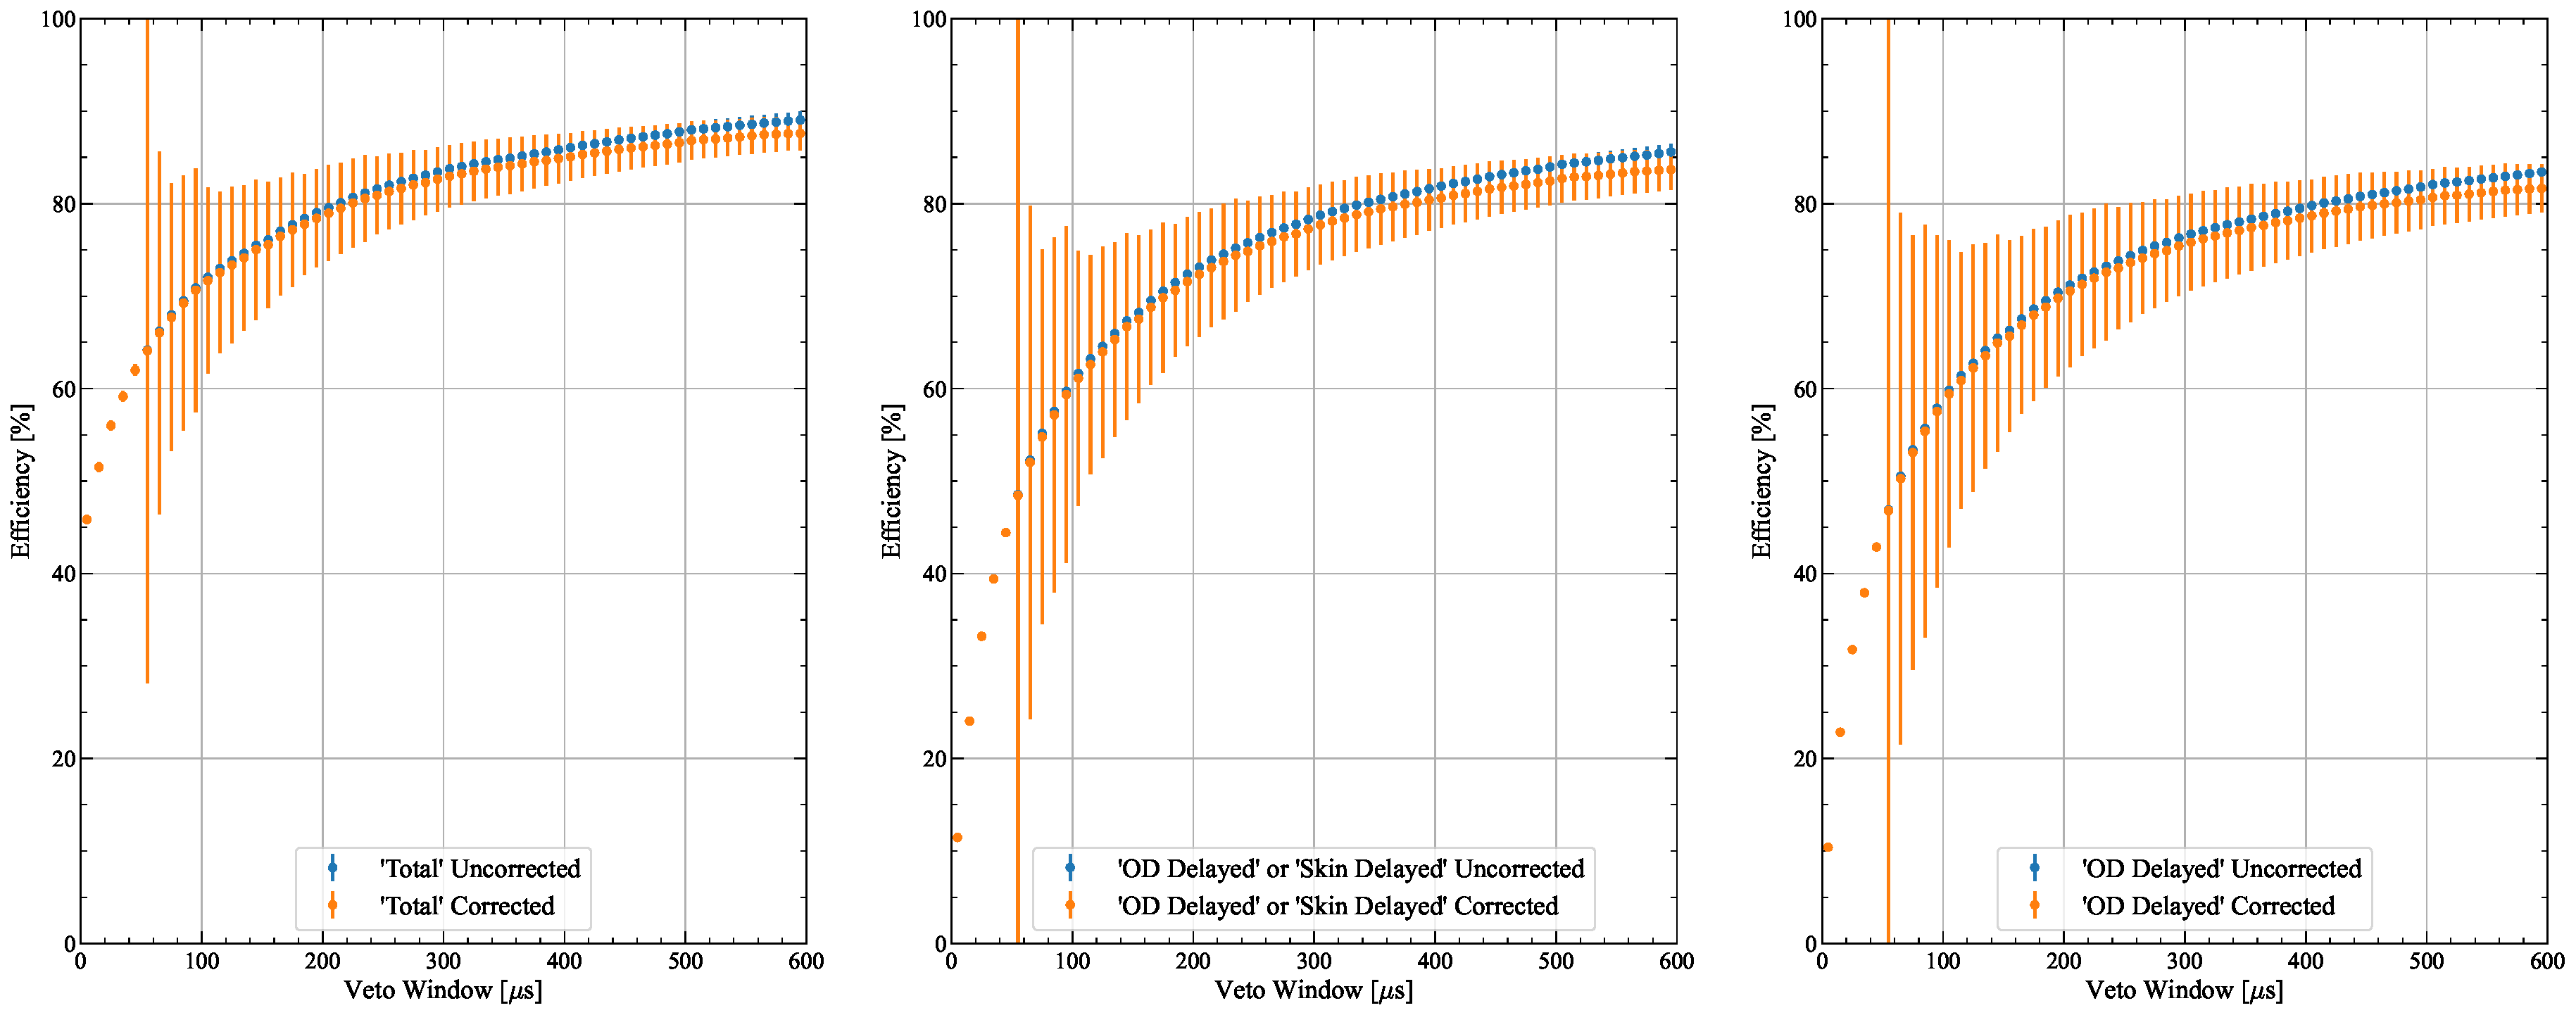
\includegraphics[width=\textwidth]{figures/VetoEfficiency/DDAccCorrectionParameters.pdf}
	\caption{The impact of the accidental correction applied to the different veto efficiencies for the given windows of interest.}
	\label{fig:VetoEff/DDAccCorrectionParameters}
\end{figure}

\subsection{Simulated neutrons from calibration sources}
AmLi and DD were simulated using \lstinline{BACCARAT-6.3.5} and \lstinline{LZLAMA-3.5.3} versions.
On each set of simulation, the cuts listed in \autoref{tab:VetoEff/calibration_simulation_efficiency_cuts} were used.
\begin{table}[!ht]
	\centering
	\caption{ALPACA-Core WS2024 cuts used on AmLi and DD simulations for determining the efficiency.}
	\begin{tabular}{l}
        \hline\hline
        \textbf{Physics cuts}              \\
        \hline
        Single scatter            \\
        S1 and S2 threshold       \\
        Fiducial Volume           \\
        CSD Selection (AmLi Only) \\
        \hline\hline
	\end{tabular}
	\label{tab:VetoEff/calibration_simulation_efficiency_cuts}
\end{table}
No accidental correction was applied to the simulation data as there are no accidental gammas or neutrons present in the simulation.
How these compare to the data measurements are shown in \autoref{fig:VetoEff/AmLiIneffPlots}-\ref{fig:VetoEff/DDIneffPlots}.
%More detailed plots on how the calibration simulations compare to calibration data is in \autoref{sec:VetoEff/simulation_improvements}.
%TODO: Should I make the comparison between data and sim with respect to what Alberto did
\begin{figure}[!ht]
	\centering
	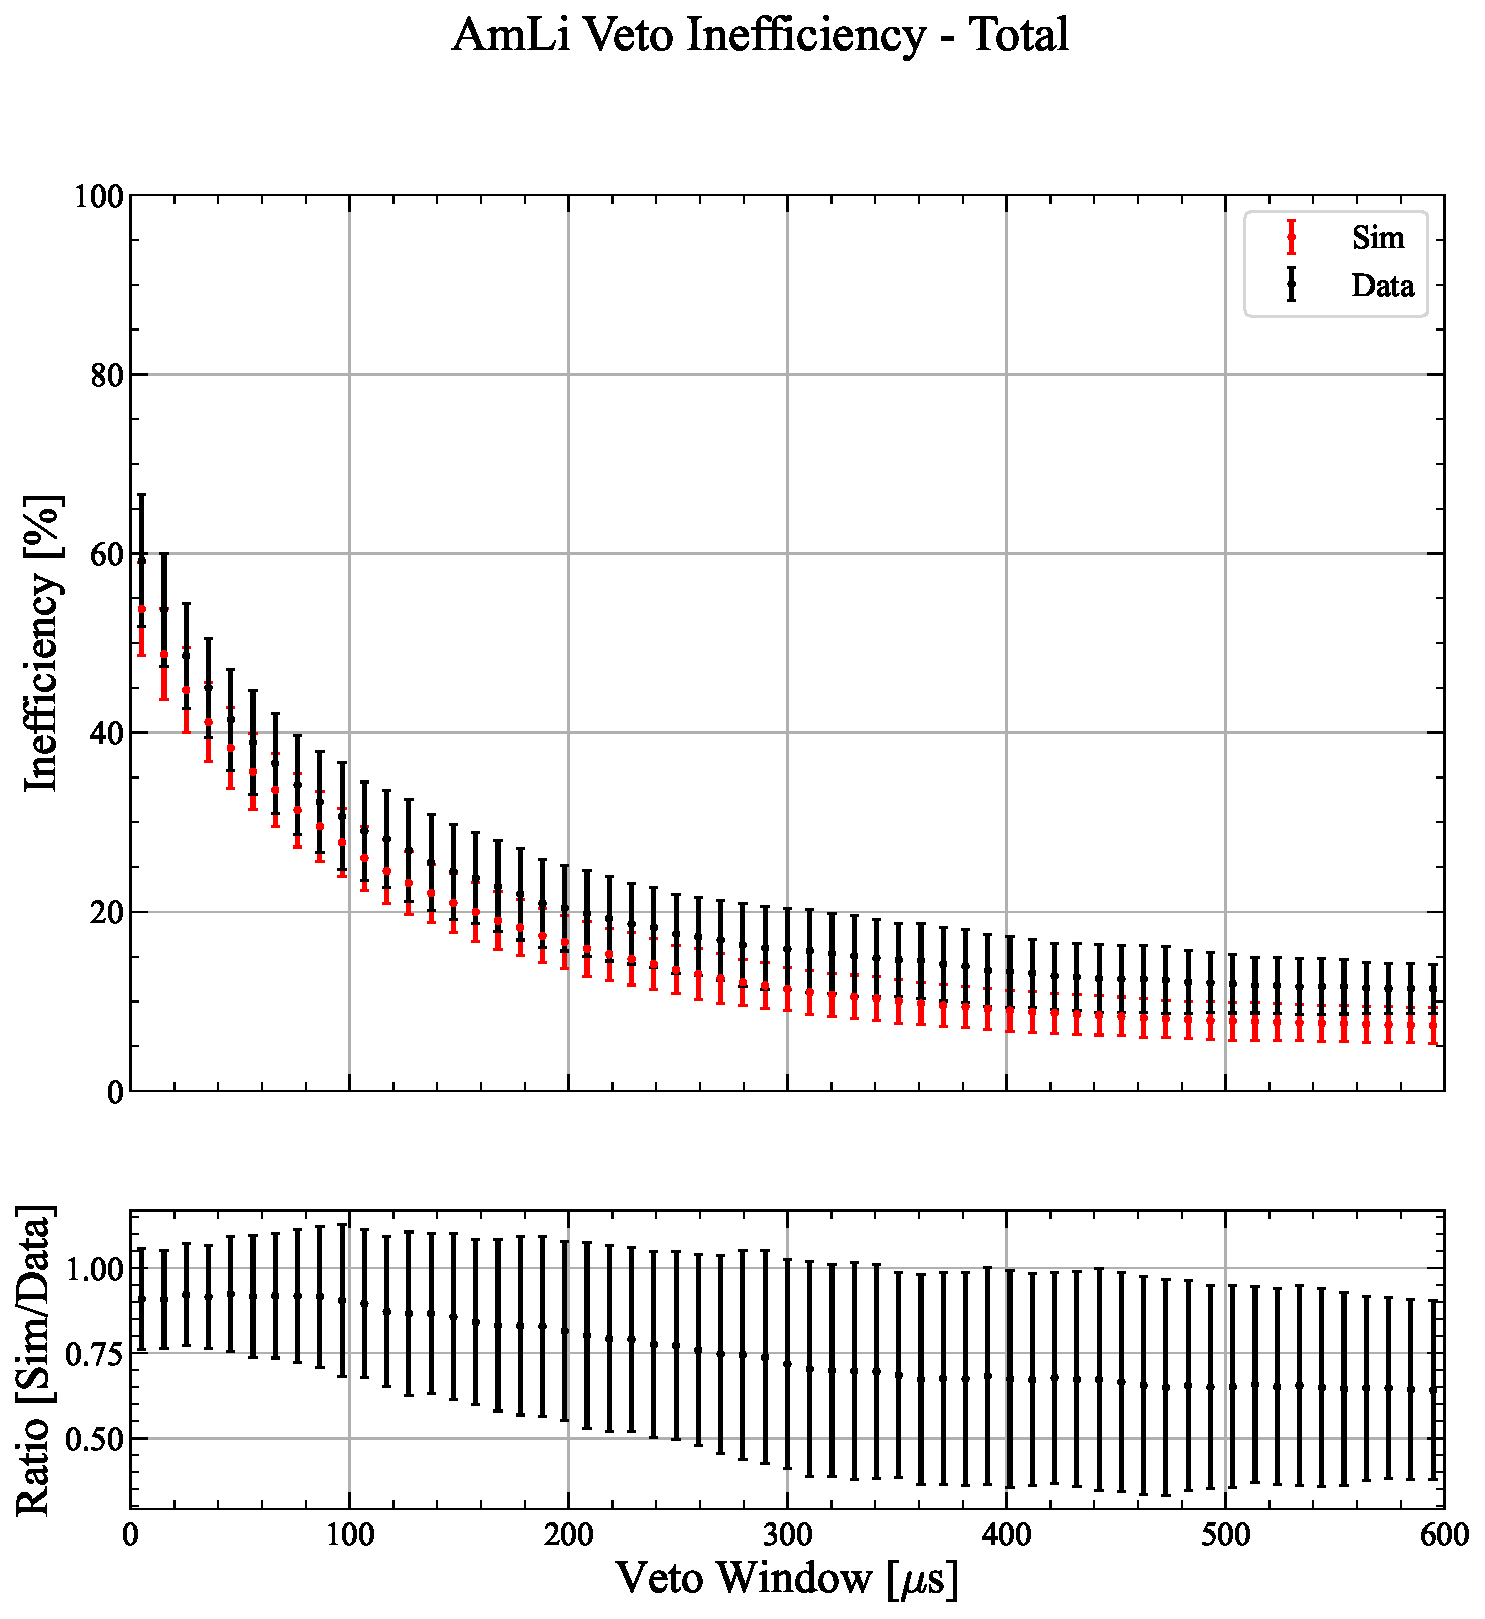
\includegraphics[width=.3\textwidth]{figures/VetoEfficiency/InEff_AmLi_Total_Avg_Ratio.pdf}\hfill
	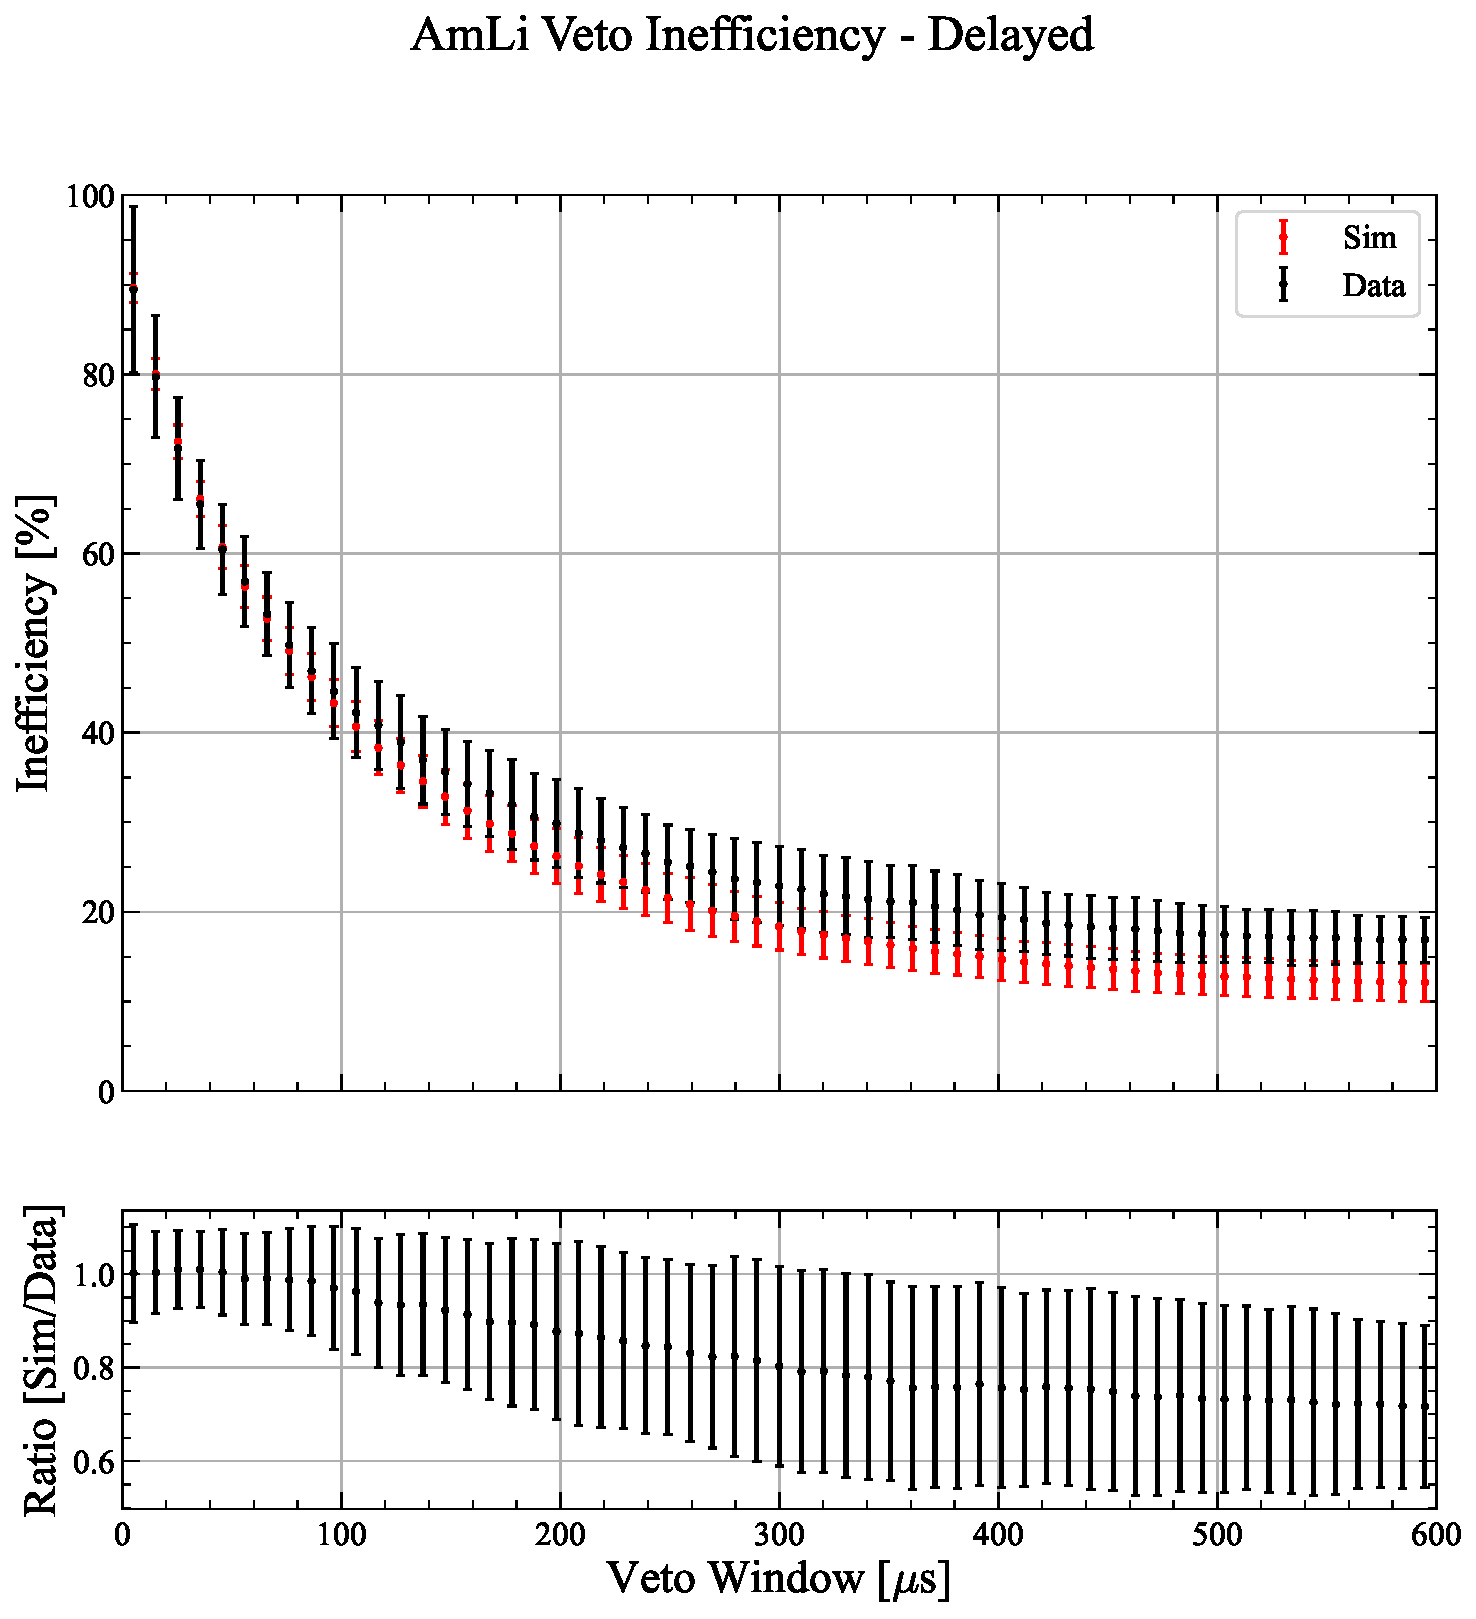
\includegraphics[width=.3\textwidth]{figures/VetoEfficiency/InEff_AmLi_Delayed_Avg_Ratio.pdf}\hfill
	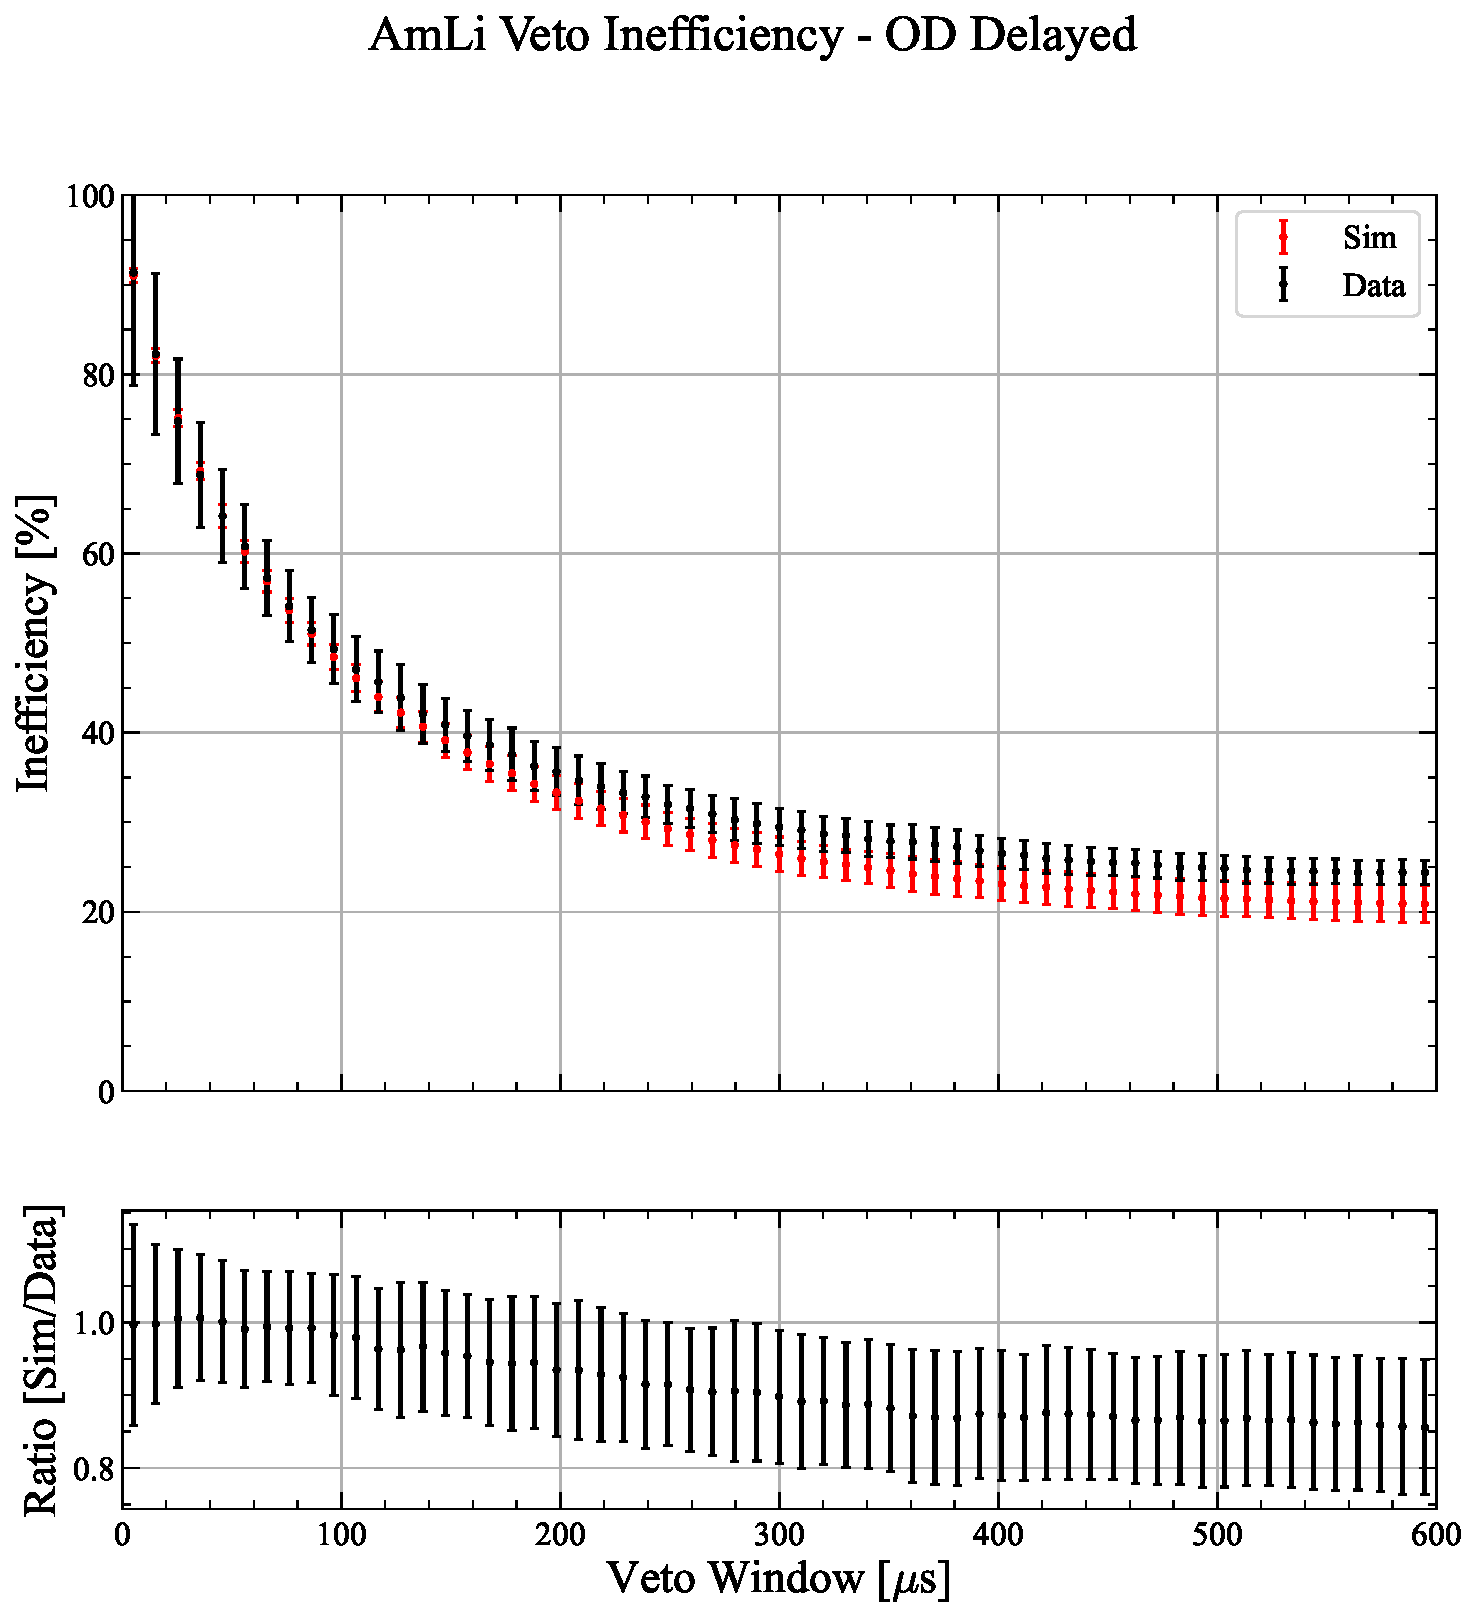
\includegraphics[width=.3\textwidth]{figures/VetoEfficiency/InEff_AmLi_ODDelayed_Avg_Ratio.pdf}
	\caption{Inefficiency plots for AmLi, comparing simulations to data.
		Left: Total. Middle: Delayed Only. Right: OD Delayed.\\
		In each case, the average from all CSD positions are used.}
	\label{fig:VetoEff/AmLiIneffPlots}
\end{figure}

\begin{figure}[!ht]
	\centering
	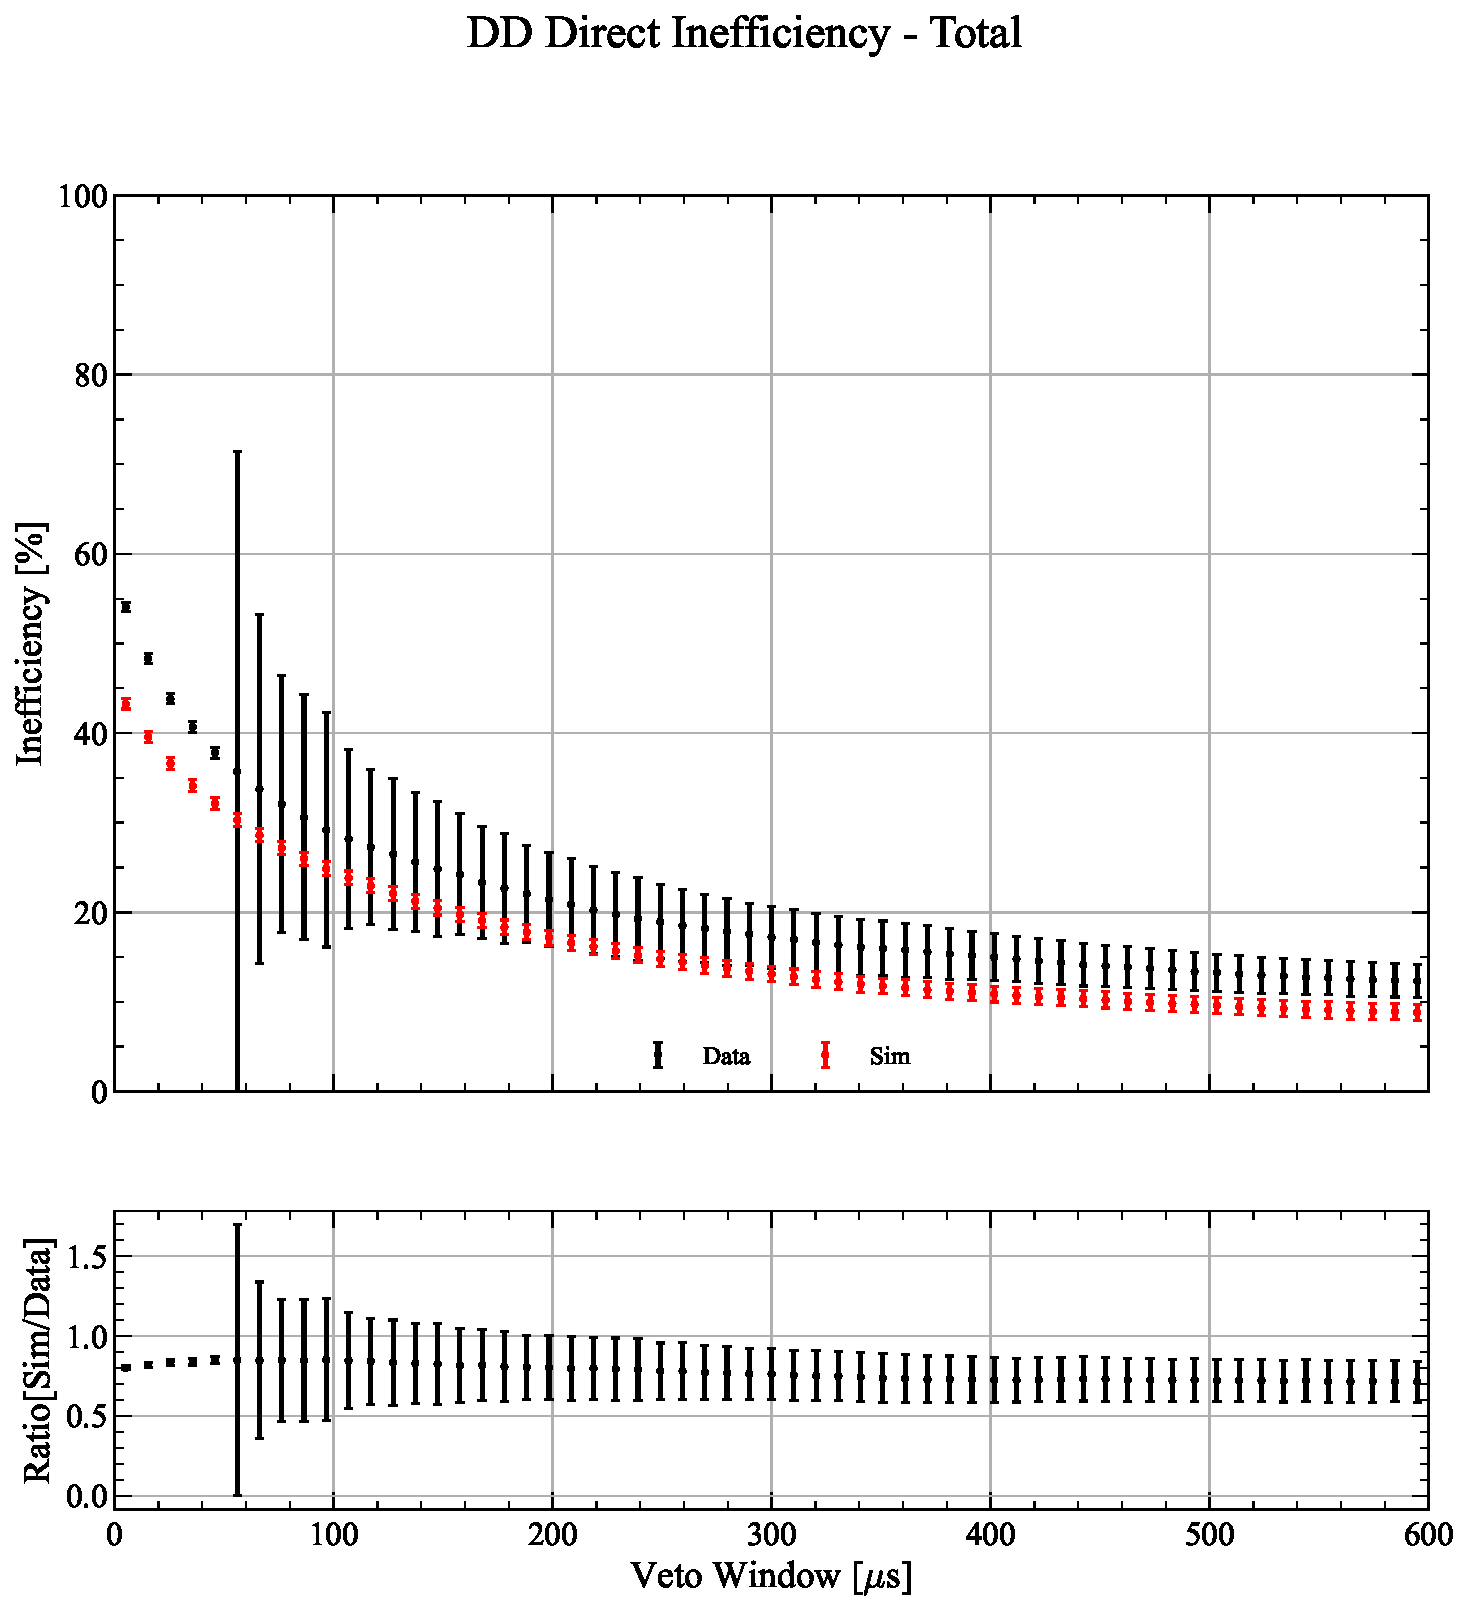
\includegraphics[width=.3\textwidth]{figures/VetoEfficiency/InEff_DDDirect_Total_Ratio.pdf}\hfill
	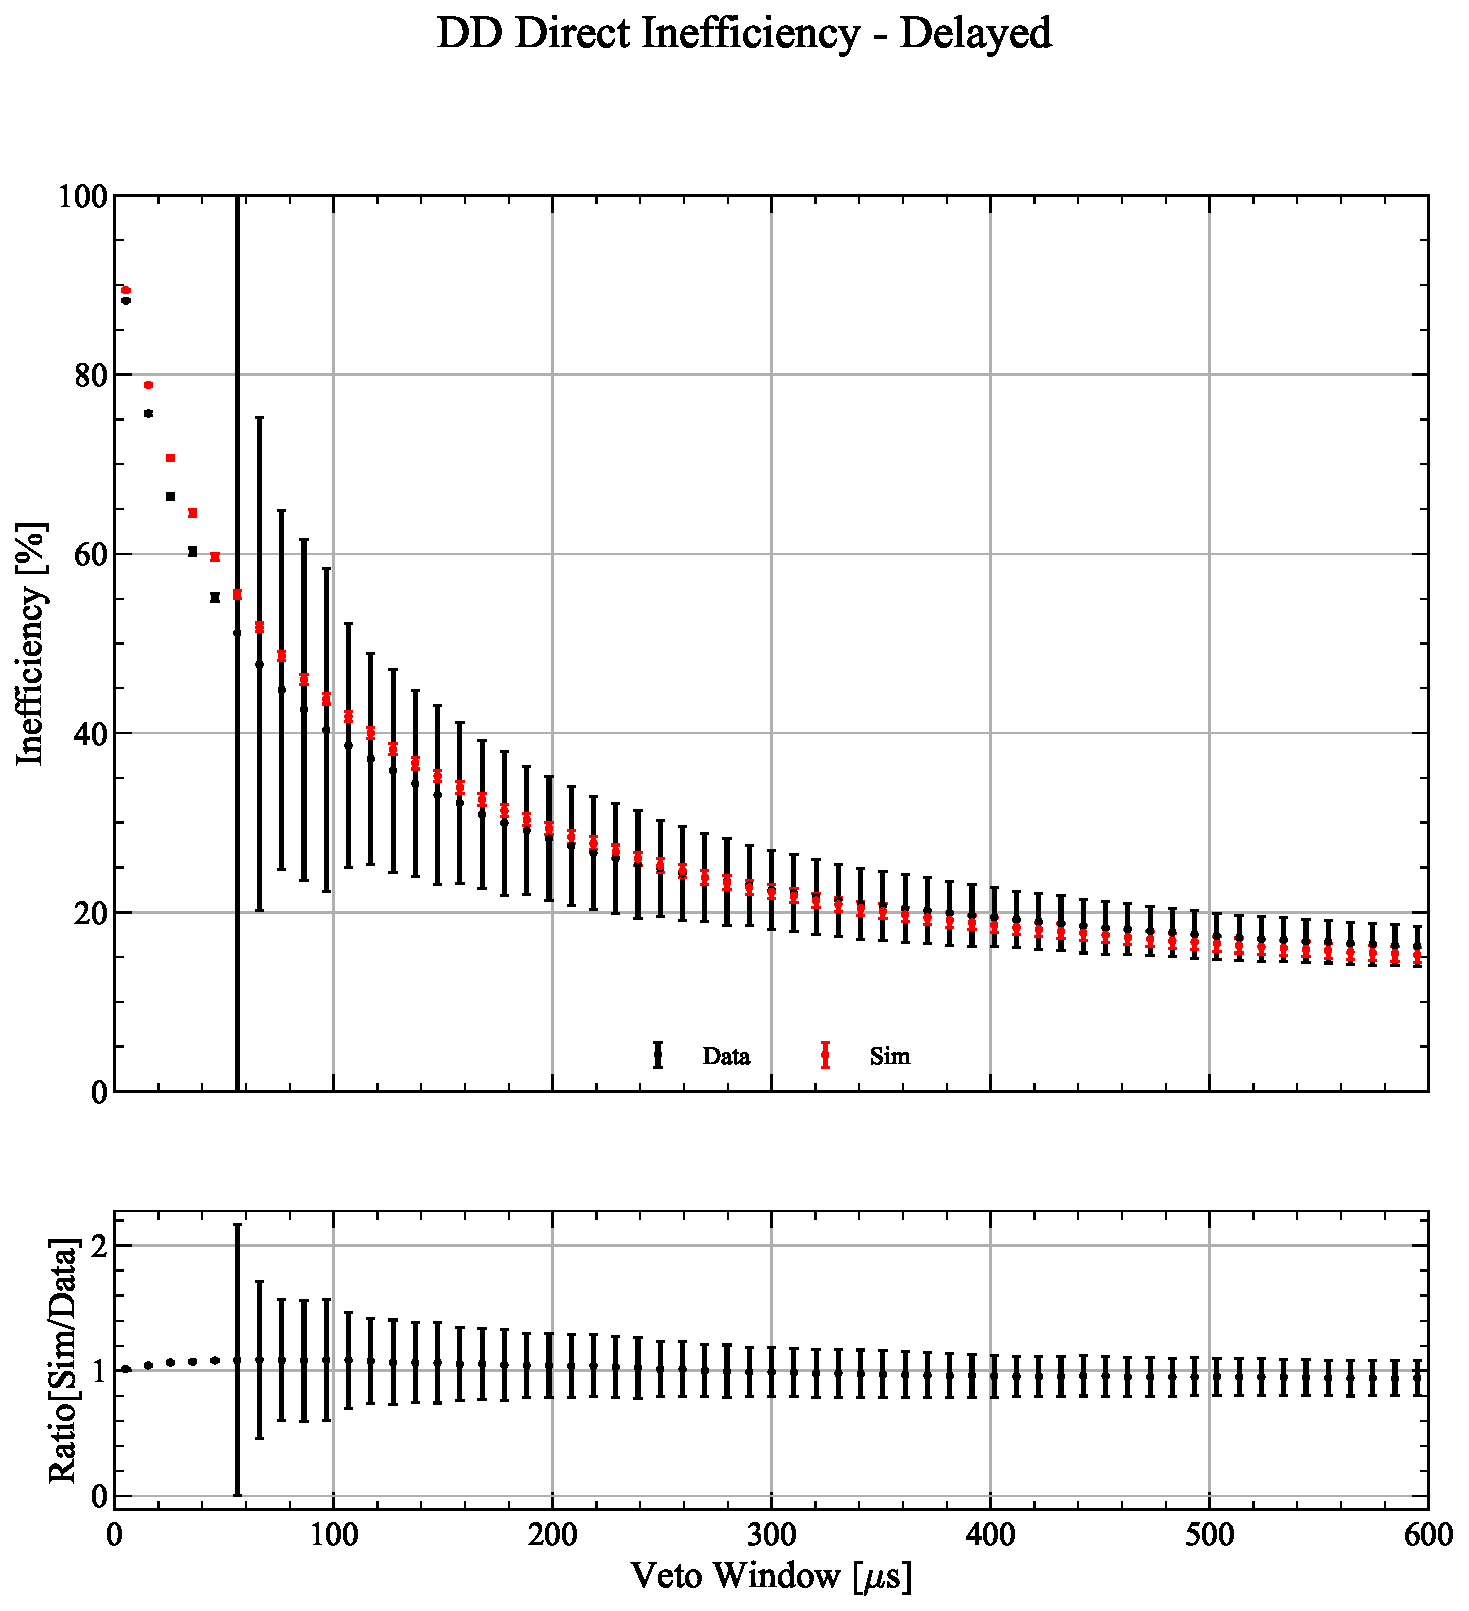
\includegraphics[width=.3\textwidth]{figures/VetoEfficiency/InEff_DDDirect_Delayed_Ratio.pdf}\hfill
	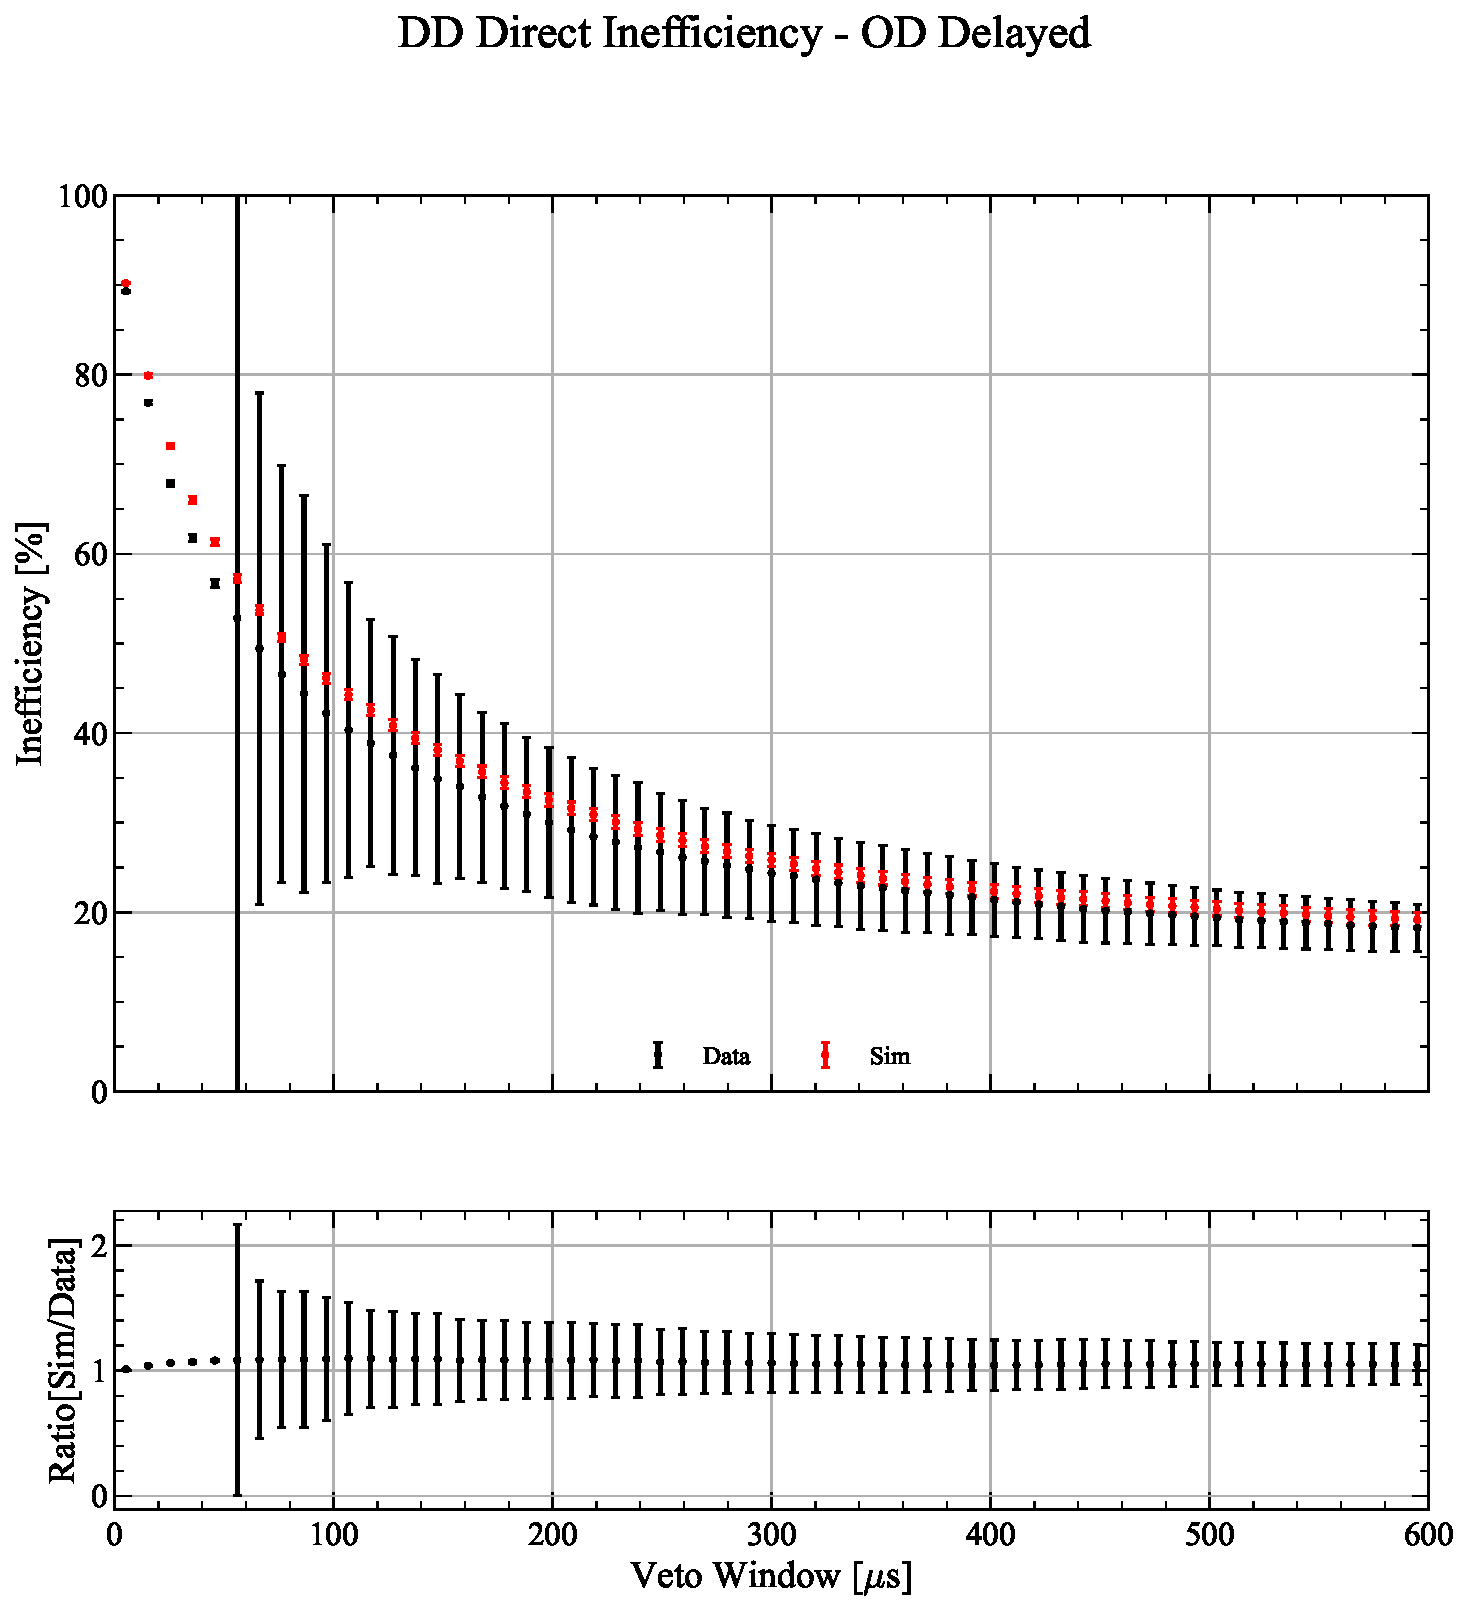
\includegraphics[width=.3\textwidth]{figures/VetoEfficiency/InEff_DDDirect_ODDelayed_Ratio.pdf}
	\caption{\centering Inefficiency plots for DD, comparing simulations to data.\\ Left: Total. Middle: Delayed Only. Right: OD Delayed.}
	\label{fig:VetoEff/DDIneffPlots}
\end{figure}

\subsection{Background neutrons}
The detector-NR simulations were simulated as part of the official production of SR3-BG. Each of the 644 components were simulated using BACCARAT-6.3.5 and LZLAMA-3.5.3 versions.
The cuts listed in \autoref{tab:VetoEff/detector_nr_simulation_efficiency_cuts} were applied.
The efficiency of tagging neutrons from Uranium Spontaneous Fission (USF) and ($\alpha$,n) events are shown in \autoref{fig:VetoEff/detector_nr_efficiency}.
Also shown is the total efficiency.

\begin{table}[!ht]
	\centering
	\caption{ALPACA-Core WS2024 cuts used on Detector-NR simulations for determining the efficiency. Each cut is from WS2024-cuts-v3.}
	\begin{tabular}{l}
    \hline\hline
		\textbf{Physics cuts}        \\
		\hline
		Single scatter      \\
		S1 and S2 threshold \\
		Fiducial Volume\\
        \hline\hline
	\end{tabular}
	\label{tab:VetoEff/detector_nr_simulation_efficiency_cuts}
\end{table}

\begin{figure}[!ht]
	\centering
	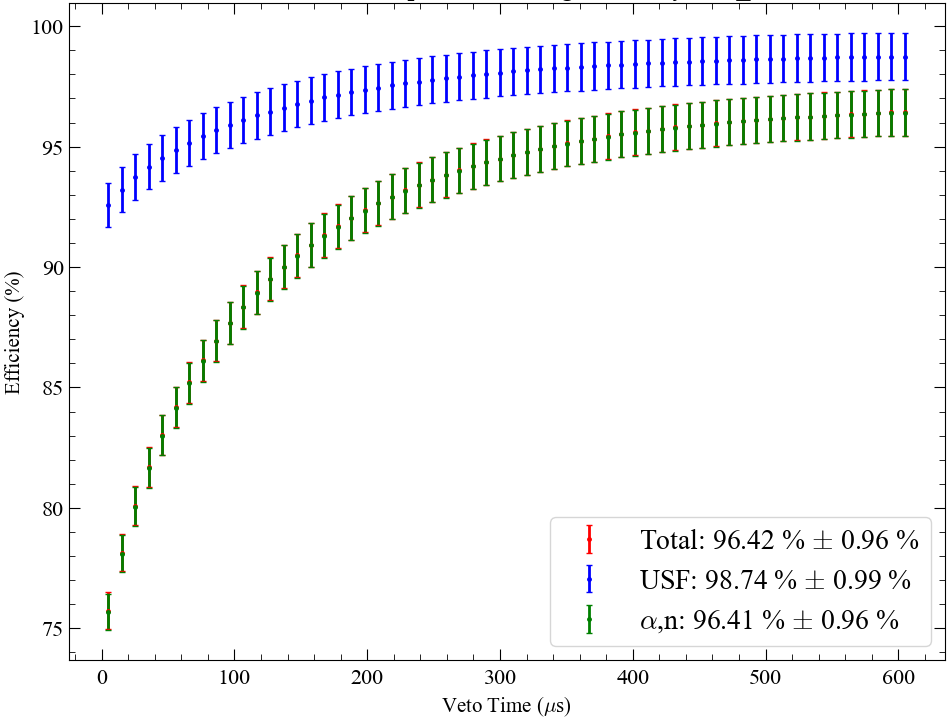
\includegraphics[width=0.7\textwidth]{figures/VetoEfficiency/det_nr_efficiency.png}
	\caption{Efficiency for tagging a neutron on Detector-NR simulations.}
	\label{fig:VetoEff/detector_nr_efficiency}
\end{figure}

\clearpage
\subsection{Background neutron efficiency from data}\label{sec:VetoEff/BkgNeutronEff}
The neutron veto efficiency from each calibration source from data and simulation is shown in \autoref{fig:VetoEff/efficiency_summary}.
Also shown is the efficiency from simulated background neutrons.
The Z-position of each point is calculated from the \lstinline{mean(driftTime)} of events which pass the selection.
For the Detector-NR, the events were split up into Z-sections by the following;
\begin{lstlisting}[backgroundcolor = \color{lightgray},language = Python]
def SR3ZThirds_Cut(driftTime_us: float, position='top'):
    if position == 'top':
        return ((driftTime_us < 350.) & (driftTime_us > 71.))
    elif position == 'mid':
        return ((driftTime_us < 700.) & (driftTime_us > 350.))
    elif position == 'bot':
        return ((driftTime_us < 1030.) & (driftTime_us > 700.))
\end{lstlisting}
This \lstinline{driftTime} splitting was performed so that comparing to calibration points was easier, but in evaluating the total efficiency, it was not used.
Shown in \autoref{tab:VetoEff/final_veto_efficiency} are the veto efficiencies of all calibration sources for both simulations and data.
The value of importance is the background neutron efficiency, $\epsilon_{\textrm{bg data}}$, or inefficiency, $\zeta_{\textrm{bg data}}$.
There are a number of ways in which this can be calculated, which are described below.
The option 2 was used for the final WS2024 result, of 7.8$\pm$4.3\%; or quote as 8$\pm$4.
\autoref{tab:VetoEff/efficiency_options} contains the results of each approach.
\paragraph{Option 1}:
The average simulation calibration efficiency was taken, so the mean of AmLi (92.8\%) and DD (91.8\%), resulted in an average efficiency of 92.3\%.
The average data calibration efficiency was taken, so the mean of AmLi (88.6\%) and DD (87.7\%), resulted in an average of 88.2\%.
The ratio, $\Delta$, of the simulation calibrations and the data calibration can then be used as a scaling factor on the simulation background.
This process is expressed in \autoref{eqn:VetoEff/:efficiency_option1}, and gives an efficiency of 92.1\%.
In this case, the uncertainty is 4.5\%, made up from a statistical error from the simulations (0.96\%), and 4.3 from the scaling.
\begin{align}
	\epsilon_{\textrm{cal. data}} & = \frac{\epsilon_{\textrm{data DD}} + \epsilon_{\textrm{data AmLi}}}{2} \\
	\epsilon_{\textrm{cal. sims}} & = \frac{\epsilon_{\textrm{sims DD}} + \epsilon_{\textrm{sims AmLi}}}{2} \\
	\Delta                        & = \frac{\epsilon_{\textrm{cal. data}}}{\epsilon_{\textrm{cal. sims}}}   \\
	\epsilon_{\textrm{bg data}}   & = \Delta \times \epsilon_{\textrm{bg sims}}
	\label{eqn:VetoEff/:efficiency_option1}
\end{align}

\paragraph{Option 2}:
The average simulation calibration efficiency was taken, mean of AmLi (92.8\%) and DD (91.8\%) resulted in an average efficiency of 92.3\%.
The average data calibration efficiency was taken, mean of AmLi (88.6\%) and of DD (87.7\%), resulted in an average efficiency of 88.2\%.
The difference, $\Lambda$, between the simulation calibrations and the data calibrations can then be used as a systematic uncertainty on the simulation backgrounds.
This process is expressed in \autoref{eqn:VetoEff/:efficiency_option2}, and gives an efficiency of 92.2\%.
In this case, the uncertainty is 4.3\%, made up from a statistical error from the simulations (0.96\%), and 4.22 from the subtraction.

\begin{align}
	\epsilon_{\textrm{cal. data}} & = \frac{\epsilon_{\textrm{data DD}} + \epsilon_{\textrm{data AmLi}}}{2} \\
	\epsilon_{\textrm{cal. sims}} & = \frac{\epsilon_{\textrm{sims DD}} + \epsilon_{\textrm{sims AmLi}}}{2} \\
	\Lambda                       & = \epsilon_{\textrm{cal. sims}} - \epsilon_{\textrm{cal. data}}         \\
	\epsilon_{\textrm{bg data}}   & = \epsilon_{\textrm{bg sims}} - \Lambda
	\label{eqn:VetoEff/:efficiency_option2}
\end{align}

\paragraph{Option 3}:
The average simulation calibration inefficiency was taken, the mean of AmLi ($100 - 92.8 = 7.2$\%) and DD ($100 - 91.8 = 8.3$\%), resulted in an inefficiency of 7.7\%.
The average data calibration inefficiency was taken, the mean of AmLi (11.5\%) and DD (12.3\%), resulted in an average inefficiency of 11.9\%.
The ratio, $\Delta$, of the simulation calibrations and the data calibration can then be used as a scaling factor on the simulation background.
This process is expressed in \autoref{eqn:VetoEff/:efficiency_option3}, and gives an inefficiency of 5.5.
In this case, the uncertainty is 2.8\%, made up from a statistical error from the simulations (0.96\%), and 1.8 from the subtraction.

\begin{align}
	\zeta_{\textrm{cal. data}} & = 100 - \frac{\epsilon_{\textrm{data DD}} +\epsilon_{\textrm{data AmLi}}}{2}  \\
	\zeta_{\textrm{cal. sims}} & = 100 - \frac{\epsilon_{\textrm{sims DD}} + \epsilon_{\textrm{sims AmLi}}}{2} \\
	\Delta                     & = \frac{\zeta_{\textrm{cal. data}}}{\zeta_{\textrm{cal. sims}}}               \\
	\zeta_{\textrm{bg data}}   & = \zeta_{\textrm{bg sims}} \times \Delta
	\label{eqn:VetoEff/:efficiency_option3}
\end{align}

\begin{table}[!ht]
	\centering
	\caption{Summary of veto efficiencies. The Detector-NR Data value assumes that option 2 is used.}
	\begin{tabular}{lll}
    \hline\hline
    \textbf{Source}& \textbf{Simulation}& \textbf{Data}\\ 
    \hline
    AmLi (average) & 92.8$\pm$2.0\% & 88.6$\pm$2.7\% \\
    DD (Direct)    & 91.8$\pm$1.0\% & 87.7$\pm$1.8\% \\
    Detector-NR    & 96.4$\pm$1.0\% & 92.2$\pm$4.3\\
    \hline\hline
	\end{tabular}
	\label{tab:VetoEff/final_veto_efficiency}
\end{table}

\begin{table}[!ht]
	\caption{Summary of veto efficiencies and inefficiencies as determined from each approach discussed in \autoref{sec:VetoEff/BkgNeutronEff}.}
	\centering
	\begin{tabular}{lll}
		\hline\hline
        \textbf{Option} & \textbf{Efficiency}& \textbf{Inefficiency} \\ 
        \hline
		1  & 92.1$\pm$4.5 & 7.9$\pm$4.5  \\
		2  & 92.2$\pm$4.3 & 7.8$\pm$4.3  \\
		3  & 94.5$\pm$2.8 & 5.5$\pm$2.8 \\
        \hline\hline
	\end{tabular}
	\label{tab:VetoEff/efficiency_options}
\end{table}

\begin{figure}[!ht]
	\centering
	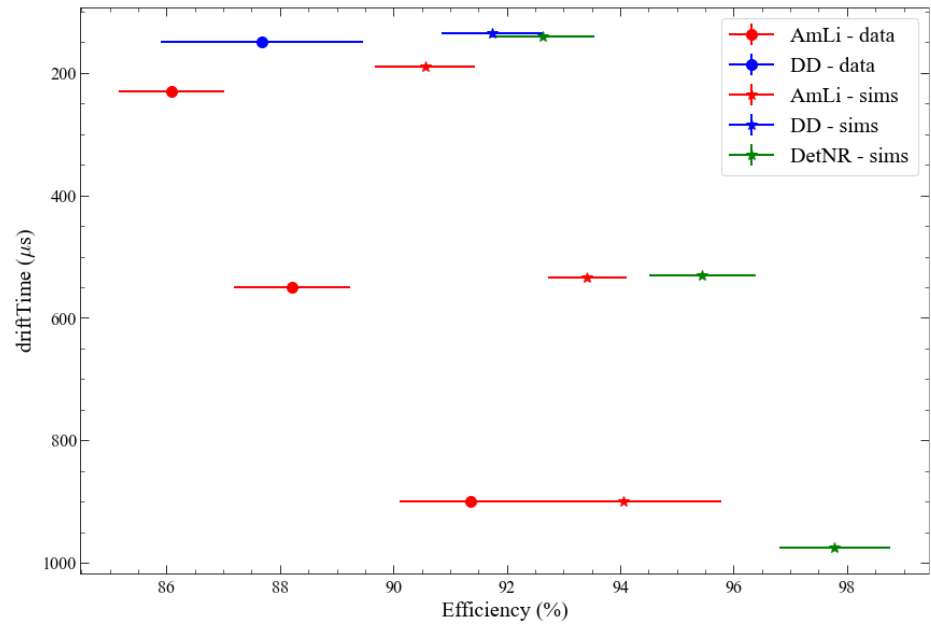
\includegraphics[width=0.7\textwidth]{figures/VetoEfficiency/efficiency_summary.png}
	\caption{Summary of efficiency from all simulations and calibration sources.
		The CSD sources are averaged at each height.
		Circle marks are from data.
		Start marks are from simulations.
		The \lstinline{driftTime} is defined as when \lstinline{mean(driftTime)} of events which pass all other cuts.
	}
	\label{fig:VetoEff/efficiency_summary}
\end{figure}

\section{Veto efficiency and the WIMP search}\label{sec:VetoEff4WIMPSearch}
\textcolor{red}{ToDo Need to talk about how the neutron efficiency is used in the WS result?}